\documentclass{article}
\usepackage{microtype}
\usepackage{graphicx}
\usepackage{booktabs}
\usepackage{hyperref}
\usepackage{xurl}
\usepackage{icml2026}
\usepackage{amsmath,amssymb,amsthm,mathtools}
\usepackage{array}
\usepackage{float}
\hypersetup{pdftitle={The Statistical Value of Adaptive Feature Queries},pdfauthor={Anonymous Authors},pdfsubject={Anonymous review manuscript on statistical model evaluation}}
\icmltitlerunning{The Statistical Value of Adaptive Feature Queries}
\newtheorem{theorem}{Theorem}
\newtheorem{proposition}[theorem]{Proposition}
\newtheorem{corollary}[theorem]{Corollary}
\newtheorem{lemma}[theorem]{Lemma}
\newcommand{\E}{\mathbb{E}}
\newcommand{\Var}{\operatorname{Var}}
\newcommand{\sgn}{\operatorname{sgn}}
\newcommand{\KL}{D_{\mathrm{KL}}}
\newcommand{\X}{\mathcal X}
\newcommand{\A}{\mathcal A}
\newcommand{\G}{\mathcal G}
\newcommand{\Hh}{\mathcal H}
\newcommand{\U}{\mathsf U}
\newcommand{\ip}[2]{\langle #1,#2\rangle_\mu}
\newcommand{\PP}{\mathbb P}
\newcommand{\pos}[1]{(#1)_+}
\newcommand{\rin}{R_{\mathrm{branch}}}
\newcommand{\rfix}{R_{\mathrm{fixed}}}
\newcommand{\sqdist}{\operatorname{dist}}
\lefthyphenmin=3
\righthyphenmin=3
\begin{document}
\twocolumn[
\icmltitle{The Statistical Value of Adaptive Feature Queries}
\begin{icmlauthorlist}
\icmlauthor{Anonymous Authors}{anon}
\end{icmlauthorlist}
\icmlaffiliation{anon}{Anonymous Institution}
\icmlcorrespondingauthor{Anonymous Author}{anonymous@example.org}
\icmlkeywords{model evaluation, adaptive feature acquisition, statistical learning theory, minimax estimation, rounds of adaptivity}
\vskip 0.3in
]
\printAffiliationsAndNotice{}

\begin{abstract}
Questionnaires limit respondent burden, clinics limit tests per patient, and budgeted classifiers limit acquisitions per input, so many population quantities must be estimated from records that each reveal only $b$ of $m$ features. We quantify what a collector gains by choosing each question after seeing earlier answers instead of pre-committing to a feature set, when the target is a population functional such as the accuracy of a frozen rule or the gain of a model update. For any menu of query protocols the first-order minimax constant is a finite convex program whose converse holds for biased and sequential estimators. Pre-committed forms need at most $2^{b-1}$ times as many records as branching interviews, and this is sharp. The gain accrues over rounds: $r$ batches of questions lose at most a factor $2^{b-r}$, and a binary pointer-tree contrast shows that this is tight up to polynomial factors in $b$, so two rounds can lose almost the whole exponent and $\Omega(b/\log b)$ rounds are needed to come within polynomial factors of full branching. At a given population the gain lies between the inverse energy explained by the best single form and the effective number of question paths of the branching tree, and certified column generation computes it exactly over all depth-$b$ trees. On retrained random-forest updates and survey screening trees the realized gain is a factor between one and two; it is stable under the smoothing and resampling of the evaluation law, is detected in advance by the bracket, and is largely missed by branching designs restricted to the models' own trees. The completion-only path-guessing baseline of the classical adaptivity simulation needs up to 25 times as many respondents; optimized pre-committed scores remove all but the intrinsic part of that cost.
\end{abstract}

\section{Introduction}
Population quantities are often estimated from records that each reveal only a few features. Questionnaires cap respondent burden, clinical protocols cap the tests ordered per patient, and budgeted classifiers acquire only a few inputs per case at deployment \citep{turney1995,trapeznikov2013,nan2017}. Two kinds of collection respect such a cap. A collector can pre-commit to a feature set for each record, as in split questionnaires, matrix sampling and fixed laboratory panels \citep{raghunathan1995,chipperfield2009}. Alternatively, it can choose each question after seeing earlier answers, as in skip logic, sequential testing and the acquisition path of a decision tree. This paper asks how many more records pre-commitment costs when the target is a population quantity such as the accuracy of a frozen screening rule or the accuracy gain of a model update.

Classical adaptivity results measure queries per input. A depth-$b$ decision tree is simulated non-adaptively by reading all of its $2^b-1$ nodes, and the huge-object model separates adaptive and non-adaptive testers by their query counts \citep{goldreich2022,chakraborty2023,adar2024}. Under a per-record cap, the price of non-adaptivity is paid instead in the number of records. Planned-missingness theory evaluates a given form menu \citep{robins1994,tsiatis2006}, and active feature acquisition optimizes individual predictions \citep{ma2019,covert2023}. Our question compares protocol classes at their statistical optima. The answer depends on how the cap is imposed, on how many rounds of questions are allowed, and on the population.

\paragraph{Contributions.}
\begin{itemize}\itemsep1pt\parskip0pt
\item \emph{Exact characterization (Theorem~\ref{thm:char}).} For any finite menu of interviews, the first-order minimax constant is a finite convex program. Its converse holds for biased estimators, for cross-record adaptation and for interview choices that see the current label, and a finite-sample version characterizes the minimax risk within a universal constant for every contrast, identifiable or not.
\item \emph{Sharp worst-case value (Theorem~\ref{thm:universal}).} Pre-committed forms need at most $\min\{2^{b-1},\binom{m-1}{b-1}\}$ times as many records as branching, with equality at an address contrast. The full exponent is nearly attained already when $m\le b^2$. Under a mean instead of a maximum budget the ratio is at most $m/b$.
\item \emph{Rounds of adaptivity (Theorem~\ref{thm:rounds}).} With $r$ batches the loss is at most $2^{b-r}$. Pointer-chasing contrasts separate $r$ from $r+1$ rounds, and a binary pointer tree shows that $r$ rounds can lose a factor $2^{b-1}/(3b)^r$: the exponent of the $r$-round gap is $b-O(r\log b)$, so a bounded number of rounds loses almost the whole exponent and $\Omega(b/\log b)$ rounds are necessary to come within polynomial factors of branching.
\item \emph{Population-specific value (Theorem~\ref{thm:bracket}).} The gain at a given population lies between the inverse energy that the best single form explains and the R\'enyi effective number of the branching tree's question paths. Column generation with an exact dynamic-programming pricing step computes the branching constant over \emph{all} depth-$b$ trees with certified bounds, and a two-phase design learns the optimal population-specific design from the audit itself while staying exactly unbiased (Proposition~\ref{prop:selfcalmain}).
\item \emph{Experiments.} On 180 binding random-forest updates at cap three, the best pre-committed design needs a median 1.51 times (up to 1.85) as many records as the best branching design; the median is 1.31 at cap two and 1.24 at cap four with six features; the exact ratios move by at most 8\% under smoothing masses between 0.1\% and 10\% and under resampling of the evaluation records; and branching menus restricted to the forests' own trees capture a median of 17\% of the gain on the log scale. On budgeted screening questionnaires the factor reaches 1.98 on survey data and is exactly one on thyroid data, where the bracket detects the absence of a gain from reference data alone. Completion-only path guessing, the estimator behind the classical adaptivity simulation, needs up to 25 times as many respondents. When complete source records exist and the conditional law of unasked items transports, imputation closes the gap; we report this as it is.
\end{itemize}

\section{Estimand and Acquisition Protocols}\label{sec:setup}
Let $X$ take values in a finite profile space $\X$, by default $\{-1,1\}^m$, and let $Y\in\{-1,1\}$ be a label. Freeze two rules $p_0,p_1:\X\to[0,1]$ that predict $+1$ with probabilities $p_j(x)$, put $d=p_1-p_0$, and define
\begin{equation}
 \Delta(P)=\E_P[Yd(X)].\label{eq:gain}
\end{equation}
This is the accuracy difference of the two rules. For deterministic rules it is the usual thresholded accuracy difference; for probabilistic ones it is the accuracy of randomized decisions. The choice $p_0\equiv1/2$ makes $\Delta$ an affine function of the accuracy of $p_1$ alone. Brier and clipped log-loss improvements have the form $a(X)+Yc(X)$ and are handled by the same score programs (Appendix~\ref{app:metrics}). Labels are recorded for every sampled record and charged separately. The cap $b$ bounds feature queries per record.

\paragraph{Protocols.}
An interview $\iota$ maps a profile $x$ to a transcript $\ell_\iota(x)$. A \emph{fixed form} queries a coordinate set chosen before the record is seen. An \emph{$r$-round interview} queries batches $B_1,B_2(x_{B_1}),\ldots,B_r$, each chosen from the answers to earlier batches, with $\sum_s|B_s|\le b$. A \emph{branching interview} is a decision tree of depth at most $b$, that is, a $b$-round interview with one question per round. The menus satisfy $\A_{\rm fixed}=\A_1\subseteq\A_2\subseteq\cdots\subseteq\A_b=\A_{\rm branch}$. Across records, a protocol may use all previous records to choose the next interview. Our lower bounds even allow the current label to be seen first. Let $R_\A(d,n)$ denote the minimax mean squared error over protocols and estimators that use $n$ records and interviews from $\A$. Figure~\ref{fig:queries} contrasts a fixed form with a tree.

\begin{figure}[t]
\centering
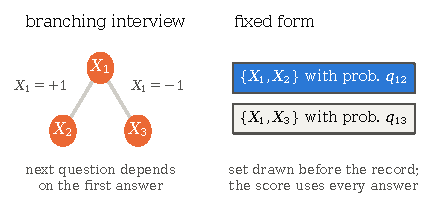
\includegraphics[width=\columnwidth]{figures/v13_protocols.pdf}
\caption{A two-query branching interview asks $X_2$ after $X_1=+1$ and $X_3$ after $X_1=-1$. A fixed form commits to $\{1,2\}$ or $\{1,3\}$ before the record is seen; it completes the tree's path only for some profiles, but its unbiased score can use every observed answer.}
\label{fig:queries}
\end{figure}

\paragraph{Identification.}
Let $\Hh_\A$ be the span of functions constant on the transcript cells of $\A$. The gain is identifiable for all populations exactly when $d\in\Hh_\A$. On the cube, fixed forms of size $b$ and depth-$b$ trees give the same condition, Fourier degree $\deg(d)\le b$ in the characters $\chi_S(x)=\prod_{j\in S}x_j$. It holds for every probability average of depth-$b$ trees, such as a depth-limited random forest, and for differences of two such ensembles, even when they use many features. Thresholds and nonlinear links can raise the degree. If $d\notin\Hh_\A$, the irreducible squared error is $\delta^2$ with $\delta=\inf_{v\in\Hh_\A}\|d-v\|_\infty$, and Appendix~\ref{app:workflow} certifies such floors for trained GBDT and MLP updates.

\paragraph{Three constants.}
$V(d,\A)$ is the worst case over populations of $\lim_n nR_\A(d,n)$; $W_\A(P)$ is the smallest variance of a pointwise-unbiased design at a population $P$, and $M_\A(P)=W_\A(P)+\Delta(P)^2$ its second moment. Ratios of $V$ compare protocol classes in the worst case; ratios of $W$ compare them at $P$ and equal the ratio of records needed there.

\section{An Exact Characterization}\label{sec:general}
Choose interview probabilities $q_\iota$ and transcript tables $g_\iota$. The score $Yg_\iota(\ell_\iota(X))/q_\iota$ is unbiased for $Yd(X)$ at every profile exactly when $\sum_\iota g_\iota(\ell_\iota(x))=d(x)$ for all $x$. Define
\begin{equation}
 V(d,\A)=\inf_{\substack{q,g:\ \sum_\iota g_\iota=d}}\ \max_{x\in\X}
             \sum_\iota\frac{g_\iota(\ell_\iota(x))^2}{q_\iota},\label{eq:unbiasedprogram}
\end{equation}
where a zero-probability interview has a zero table.

\begin{theorem}[Exact characterization]\label{thm:char}
Let $\X$ and $\A$ be finite and $d\in\Hh_\A$. Then $nR_\A(d,n)\to V(d,\A)$, and an iid design with the unbiased score attains $V/n$ for every $n$. The converse applies to biased estimators, to designs that adapt across records, and to interview choices that depend on the current label. Moreover
\[
 V(d,\A)=\sup_{\mu,h}\frac{\langle d,h\rangle_\mu^2}{\max_{\iota\in\A}\|\E_\mu[h\mid\ell_\iota(X)]\|_\mu^2},
\]
over strictly positive profile laws $\mu$ and witnesses $h$ with nonzero denominator. For every contrast $d$, identifiable or not, and every $n$, the minimax risk $R_\A(d,n)$ lies within a universal factor $104$ of
\begin{equation}
 \Phi_n(d,\A)=\inf_{q,g}\max_{x\in\X}\Big[\big(d(x)-s_g(x)\big)^2+\frac1n\sum_\iota\frac{g_\iota(\ell_\iota(x))^2}{q_\iota}\Big],\!\!\label{eq:phimain}
\end{equation}
where $s_g(x)=\sum_\iota g_\iota(\ell_\iota(x))$ is the mean score at profile $x$.
\end{theorem}
Formal statements and proofs are Theorems~\ref{thm:finite}--\ref{thm:asym} (Appendices~\ref{app:generalstatements}--\ref{app:general}). The dual compares the signal $\langle d,h\rangle_\mu$ of a perturbation of the label mean with the largest projection energy that one interview can capture. A change of measure, the KL chain rule and a local van Trees argument turn this into minimax risk. These are established tools for linear functionals \citep{donoho1994,juditsky2009,polyanskiy2026} and for information-constrained estimation with a prescribed channel family \citep{acharya2019,barnes2020}; what is new is that the witness is controlled simultaneously for every interview of a menu, including label-dependent choices, which yields exact constants for \emph{comparing} query classes.

\paragraph{Approximately identifiable contrasts.}
The program \eqref{eq:phimain} trades a uniform approximation error against the variance of the approximant's score; for $d\notin\Hh_\A$ it decreases to $\delta^2$, so thresholded or link-transformed updates have minimax risk $\delta^2+\Theta(1/n)$ with constants determined by \eqref{eq:phimain}; Appendix~\ref{app:floor-rate} gives the explicit envelope $\delta^2\le R_\A(d,n)\le\inf_v\{\|d-v\|_\infty^2+V(v,\A)/n\}$ over approximants $v\in\Hh_\A$, and Appendix~\ref{app:workflow} certifies brackets of $\delta$ for GBDT and MLP updates. The exact first-order constant of the biased regime is not determined here.

\paragraph{Population-specific constants.}
For a fixed law $P$ of $(X,Y)$ and $t(x,y)=yd(x)$, let
\begin{equation}
 W_{\A}(P)=\inf_{q,H:\,\E[H\mid X,Y]=t(X,Y)}\Var_{P,q}(H),\label{eq:mainW}
\end{equation}
where the score must be unbiased at every profile and label but may be tuned to $P$. At a full-support $P$, $W_\A(P)/n$ is the local asymptotic minimax risk over \emph{arbitrary} estimators that use the capped records alone, in shrinking neighborhoods of $P$ (Proposition~\ref{prop:local}). Ratios $W_{\rm fixed}(P)/W_{\rm branch}(P)$ therefore compare protocol classes at that population for every such estimator; estimators that import complete records from another source lie outside this information set (Section~\ref{sec:experiments}).

\section{How Much Can Adaptivity Be Worth?}\label{sec:gap}
\begin{theorem}[Sharp gap]\label{thm:universal}
For $1\le b\le m$ and a nonzero contrast of degree at most $b$ on $\{-1,1\}^m$,
\begin{equation}
 1\le\frac{V_{\rm fixed}(d,b)}{V_{\rm branch}(d,b)}
 \le K_{m,b}:=\min\Big\{2^{b-1},\binom{m-1}{b-1}\Big\}.\label{eq:universal}
\end{equation}
The supremum over dimensions is $2^{b-1}$, attained at $m=b-1+2^{b-1}$. For every $b\ge2$ there is an example with $m\le b^2$ and ratio at least $2^{b-b/(\kappa+1)-\kappa}$, where $\kappa=\lfloor\log_2 b\rfloor$.
\end{theorem}

\begin{figure*}[t]
\centering
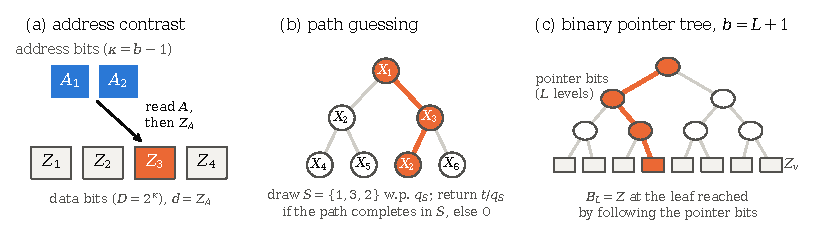
\includegraphics[width=\textwidth]{figures/v13_constructions.pdf}
\caption{The three constructions behind Theorems~\ref{thm:universal} and~\ref{thm:rounds}. (a) Address contrast: $\kappa=b-1$ address bits select one of $D=2^\kappa$ data bits; branching reads the address and then the selected bit, while any fixed set of $b$ coordinates explains at most a fraction $1/D$ of the target's energy under the uniform law, so pre-committed forms need $D$ times as many records. (b) Path guessing: a fixed form draws one of a tree's at most $2^{b-1}$ padded path sets and rescales the tree's score by $1/q_S$ when the path completes inside it; at a population, $q_S\propto w_S^{1/2}$ gives the effective number of paths $N_P$. (c) Binary pointer tree: $L=b-1$ levels of pointer bits select a child and the target is the data bit at the reached leaf; a round that reads $a$ pointer bits raises the conditional probability of the most likely leaf by at most a factor $1+2a$.}
\label{fig:constructions}
\end{figure*}

\paragraph{Proof idea.}
Pad every root-to-leaf path of a tree to $b$ distinct coordinates. Its first $b-1$ answers determine the path's coordinate set, so a tree has at most $K_{m,b}$ distinct sets. A fixed form draws one set uniformly before the record, follows the tree when it can, and multiplies a completed score by the number of sets (Figure~\ref{fig:constructions}b). The mean is unchanged and the second moment grows by at most $K_{m,b}$. For sharpness, let $\kappa=b-1$ address bits select one of $D=2^\kappa$ data bits, $d(A,Z)=Z_A$ (Figure~\ref{fig:constructions}a). Branching reads the address and then the selected bit, so $V_{\rm branch}=1$. Under the uniform law, a form $T$ with $s$ address and $r$ data bits explains energy
\begin{equation}
 \|\E[d\mid X_T]\|_2^2=r2^{s-2\kappa}\le2^{-\kappa},\qquad r+s\le\kappa+1,\label{eq:addressinformation}
\end{equation}
and the dual in Theorem~\ref{thm:char} gives $V_{\rm fixed}\ge D$. Products of address blocks keep their projection energies multiplicative even when a form reallocates queries across blocks; this gives the polynomial-dimensional example (Appendix~\ref{app:productaddress}). Both constants in \eqref{eq:universal} are worst cases over populations taken separately; Section~\ref{sec:population} compares the classes at one population.

\paragraph{Hard caps versus mean budgets.}
The exponential gap requires that \emph{every} record obey the cap. If only the expected number of queries is at most $b$, querying all $m$ features with probability $b/m$ identifies every contrast and bounds the ratio by $m/b$. For the address with cap $B$ and mean budget $b$ the exact coefficients are $V^{b,B}_{\rm fixed}=DB/[b(B-\kappa)]$ and $V^{b,B}_{\rm branch}=1$ for $\kappa+1\le b\le B\le\kappa+D$ (Proposition~\ref{prop:hybrid}), so raising the hard cap moves the ratio continuously from $D$ to $m/b$.

\begin{theorem}[Rounds of adaptivity]\label{thm:rounds}
Let $V_r$ denote the constant for $r$-round interviews with at most $b$ queries.
\textup{(a)} For every nonzero contrast of degree at most $b$ and $1\le r\le b$,
$V_{\rm branch}\le V_r\le\min\{2^{b-r},\binom{m-r}{b-r}\}V_{\rm branch}$.
\textup{(b)} For $r,\kappa\ge1$ and $b=r\kappa+1$, the pointer-chasing contrast $N_{r,\kappa}$ on $m=\Theta(2^{r\kappa})$ coordinates satisfies $V_{r+1}(N_{r,\kappa})=V_{\rm branch}(N_{r,\kappa})=1$ and $2^\kappa/b\le V_r(N_{r,\kappa})\le2^\kappa$.
\textup{(c)} For $b\ge2$, the binary pointer tree $B_{b-1}$ on $m=2^b-1$ coordinates satisfies $V_{\rm branch}(B_{b-1})=1$ and, for $2\le r\le b$,
\[
 V_r(B_{b-1})\ \ge\ \frac{2^{b-1}}{r\,b\,(1+2b/(r-1))^{r-1}}\ \ge\ \frac{2^{b-1}}{(3b)^r}.
\]
Hence $2^{b-2}/(b(2b+1))\le\sup_{m,d}V_2/V_{\rm branch}\le2^{b-2}$, and the exponent of the $r$-round gap lies between $b-1-r\log_2(3b)$ and $b-r$.
\end{theorem}

In $N_{r,\kappa}$, a $\kappa$-bit register points to one of $2^\kappa$ registers at the next level, $r$ levels deep, and the last pointer selects a data bit; following one level per round computes the contrast in $r+1$ rounds, while in $r$ rounds the selected data bit is read only by a lucky guess of probability at most $2^{-\kappa}$ per question (Appendix~\ref{app:roundshier}). This separates consecutive numbers of rounds but leaves the exponent for a fixed small $r$ open. The binary pointer tree closes most of that gap (Figure~\ref{fig:constructions}c). Its pointer bits form a complete binary tree of depth $L=b-1$ whose leaves carry the data bits, and the contrast is the data bit at the leaf reached by following the pointers; this is the tree evaluation instance of \citet{cook2012}, which \citet{li2026regex} use with a deterministic adversary to show that exact evaluation under a cap of $B$ queries per round needs $L/\lceil\log_2(B+1)\rceil$ rounds. Under a total per-record cap, exact evaluation in few rounds is impossible for every strategy, and the question becomes how much variance the shortfall costs. One question per round follows the path. For the lower bound, let $M_t$ be $2^{L}$ times the conditional probability of the most likely leaf given the transcript of the first $t$ rounds. A round that reads $a_t$ pointer bits satisfies $\E[M_t\mid\text{past}]\le(1+2a_t)M_{t-1}$, because a newly read bit can only double the probability of a leaf below it, whereas the data bit of the selected leaf can be read only with probability proportional to $M_{t-1}$. A supermartingale argument over the $r$ rounds bounds the probability of ever reading the selected data bit by $rb(1+2b/(r-1))^{r-1}2^{-L}$, and the dual of Theorem~\ref{thm:char} converts this into the bound on $V_r$ (Appendix~\ref{app:roundshier}). The bound is informative for $b\ge10$; for smaller $b$ only a constant separation $4/3$ between two rounds and branching is known, and whether the polynomial factors can be removed is open. Questionnaire pages, clinic visits and laboratory batches are rounds in this sense.

\section{The Value of Adaptivity at a Population}\label{sec:population}
The worst-case constants are attained by extremal populations. For a fixed $P$ we bracket the gain by two interpretable quantities. Let $\tau$ be a depth-$b$ tree that computes $d$, let $S_\tau(x)$ be the padded coordinate set of the path of $x$, and put $w_S=\E_P[t^2\mathbf 1\{S_\tau(X)=S\}]/\E_P[t^2]$. Define
\begin{gather*}
 N_P(\tau)=\Big(\sum_Sw_S^{1/2}\Big)^2,\\
 \Gamma_P=\max_{|T|=b}\frac{\E_P\big[\E_P[t\mid X_T,Y]^2\big]}{\E_P[t^2]}.
\end{gather*}
$N_P$ is the exponential R\'enyi entropy of order $1/2$ of the path weights: the effective number of question sets the tree uses at $P$. $\Gamma_P$ is the largest fraction of the target's energy that any single form explains.

\begin{theorem}[Population-specific bracket]\label{thm:bracket}
If a depth-$b$ tree $\tau$ computes $d$, then $M_{\rm branch}(P)=\E_P[t^2]$ and
\[
 \frac1{\Gamma_P}\ \le\ \frac{M_{\rm fixed}(P)}{M_{\rm branch}(P)}\ \le\ N_P(\tau)\ \le\ K_{m,b}.
\]
On the variance scale, with $\sigma_P^2=\E_P[t^2]-\Delta^2$ and $\Delta=\Delta(P)$,
\[
 \frac{\E_P[t^2]/\Gamma_P-\Delta^2}{\sigma_P^2}\le\frac{W_{\rm fixed}(P)}{W_{\rm branch}(P)}\le\frac{N_P(\tau)\E_P[t^2]-\Delta^2}{\sigma_P^2}.
\]
Both second-moment inequalities are equalities, with value $D$, for the address contrast under the uniform law. For every menu $\A$ and witness $h$, $M_\A(P)\ge\E_P[th]^2/\max_{\iota\in\A}\E_P[\E_P[h\mid\ell_\iota(X),Y]^2]$.
\end{theorem}

The upper bound optimizes path guessing with $q_S\propto w_S^{1/2}$. The lower bound is Cauchy--Schwarz applied to the decomposition $\sum_\iota g_\iota=t$, and the variance scale follows because every design in \eqref{eq:mainW} is unbiased (Appendix~\ref{app:population}). Adaptivity pays when the tree's questions diverge over many well-populated paths ($N_P$ large) and when no fixed set of $b$ questions explains most of the target ($\Gamma_P$ small). Correlated features and shared top splits raise $\Gamma_P$ and shrink the gain. Both ends are computable from reference data before any collection.

\paragraph{Computing the branching constant exactly.}
When no single tree computes $d$, as for a random forest, the optimal branching design mixes many trees. The program for $M_{\rm branch}(P)$ has one column per depth-$b$ tree, which for $m=12$ and $b=3$ is about $1.5\times10^7$ trees. The last inequality of Theorem~\ref{thm:bracket} makes column generation exact and certifiable. Given the dual witness $h$ of a restricted master problem, the projection energy of a tree is a sum over its leaves, so the most informative tree is found by dynamic programming over partial assignments in $O(m^b2^b)$ time. Its energy yields a lower bound on $M_{\rm branch}$ over all trees, the master value yields an upper bound, and the tree is added as a new column (Appendix~\ref{app:forestexact}). The master has $O(\binom mb2^b)$ form variables plus $2^b$ per tree; we solve it for $m\le12$ and $b\le5$, and larger menus need restricted masters with the same certificates.

\paragraph{Optimal pre-committed designs.}
The fixed class is computed by the same program restricted to forms. On the cube, pointwise unbiasedness $\sum_Tg_{T,y}(x_T)=yd(x)$ is equivalent to matching Fourier coefficients, $\sum_{T\supseteq S}\widehat g_{T,y}(S)=y\widehat d(S)$ for $|S|\le b$. The design problem
\begin{equation}
\begin{aligned}
 \min_{q,g}\ &\sum_{T,u,y}P_T(u,y)\,\frac{g_{T,y}(u)^2}{q_T}\\
 \text{s.t.}\ &\text{these identities and }\textstyle\sum_Tq_T=1
\end{aligned}\label{eq:formprogram}
\end{equation}
is a second-order cone program with $O(\binom mb2^b)$ variables that never enumerates the $2^m$ profiles. Its tables use every answer on a form and include all shared-coordinate control variates (Proposition~\ref{prop:sharing}). The identities hold at every profile, so a design fitted on reference marginals $\widehat P_T$ stays exactly unbiased when the reference is wrong, and calibration error only inflates the variance. In coarsening terms, \eqref{eq:formprogram} computes the optimal augmentation of inverse-probability weighting for the form menu jointly with the form probabilities \citep{robins1994,tsiatis2006}.

\paragraph{Learning the design without reference records.}
\begin{proposition}[Two-phase self-calibration]\label{prop:selfcalmain}
Let a pilot of $n_1\to\infty$, $n_1=o(n)$, records be interviewed with the uniform design on $\A$, let the cell masses of every interview be estimated from the pilot and smoothed by a mass $\alpha_n\to0$ with $\alpha_n n_1^{1/2}\to\infty$, and let the remaining records use the design that solves \eqref{eq:mainW} at the estimated masses with a vanishing floor on the interview probabilities. The resulting estimator is exactly unbiased for every population, and $n$ times its variance converges in probability to $W_\A(P)$.
\end{proposition}
Every cell mass is estimable from the records assigned its interview, and the pointwise constraints keep every fitted design unbiased, so learning the design costs variance only (Appendix~\ref{app:selfcal}); in Section~\ref{sec:experiments} reference records play the role of the pilot.

\section{Experiments}\label{sec:experiments}
We compute the constants of Sections~\ref{sec:general}--\ref{sec:population} exactly for trained models. The population $P$ is the held-out empirical law mixed with a uniform mass $\alpha$ over profiles and labels, $\alpha=1\%$ unless stated; it has full support, so $W_\A(P)$ is a local minimax risk. Fixed designs range over all $\binom mb$ forms with the pointwise-unbiased score program of Appendix~\ref{sec:pathdesign}. We report $W_{\rm fixed}/W_{\rm branch}$, the factor by which the best pre-committed design needs more records. \emph{Fitted} designs are optimized on separate reference records and evaluated on $P$.

\begin{figure*}[t]
\centering
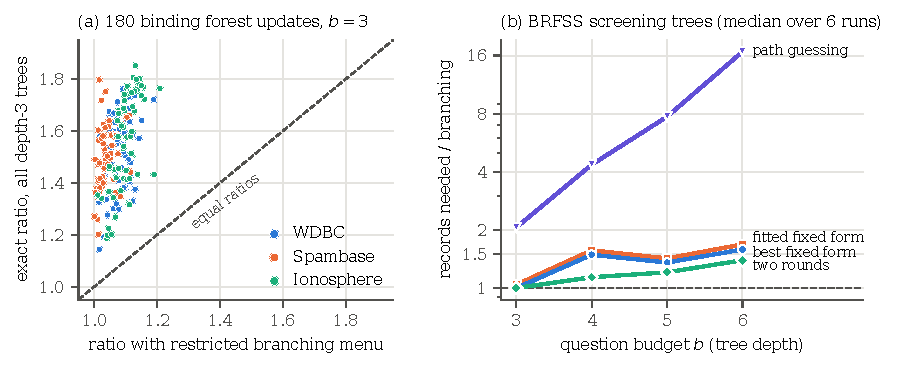
\includegraphics[width=\textwidth]{figures/v12_main.pdf}
\caption{(a) Exact fixed/branching variance ratios for the 180 binding forest updates at cap $b=3$ against the ratio obtained when branching is restricted to the forests' own 40 component trees and all triples. (b) BRFSS screening trees: records needed relative to branching, median over two targets and three seeds.}
\label{fig:v12main}
\end{figure*}

\paragraph{Independently retrained forests.}
On WDBC, Spambase and Ionosphere \citep{wolberg1993,spambase1999,ionosphere1989}, twenty splits each fit an old and a new forest of twenty depth-$b$ trees on disjoint training records, using 3, 6, 9 or 12 median-binarized features. At cap $b=3$ the 180 tasks with more than three candidate features are binding, and column generation over all depth-3 trees converged on every task to certified relative error $10^{-6}$.

\begin{table}[t]
\centering
\caption{Independent forest updates, cap $b=3$, 20 splits per cell. Exact fixed/branching variance ratio over all forms and all depth-3 trees (median and 10th--90th percentiles). Restr.: branching restricted to the 40 component trees and all triples. Fix/full: fixed-form variance relative to the full-information variance. Fitted: designs optimized on training records, evaluated held-out ($m=12$, five splits).}
\label{tab:forestexact}
\footnotesize
\setlength{\tabcolsep}{2.6pt}
\begin{tabular}{llrrrr}
\toprule
Data & $m$ & Exact ratio & Restr. & Fix/full & Fitted \\
\midrule
WDBC & 6 & 1.36 [1.27, 1.48] & 1.08 & 2.11 &  \\
 & 9 & 1.57 [1.43, 1.69] & 1.09 & 3.91 &  \\
 & 12 & 1.66 [1.53, 1.74] & 1.08 & 5.55 & 1.67 \\
Spambase & 6 & 1.41 [1.27, 1.52] & 1.03 & 2.31 &  \\
 & 9 & 1.45 [1.36, 1.59] & 1.03 & 3.09 &  \\
 & 12 & 1.58 [1.49, 1.66] & 1.04 & 4.75 & 1.60 \\
Ionosphere & 6 & 1.36 [1.20, 1.46] & 1.07 & 2.06 &  \\
 & 9 & 1.61 [1.45, 1.77] & 1.10 & 4.19 &  \\
 & 12 & 1.73 [1.58, 1.78] & 1.10 & 5.94 & 1.79 \\
\bottomrule
\end{tabular}
\end{table}


Table~\ref{tab:forestexact} and Figure~\ref{fig:v12main}(a) give three findings. First, adaptivity is worth a median factor 1.51 over the 180 binding tasks (maximum 1.85), and the factor grows with the number of candidate features. Second, a branching menu built from the forests' own component trees captures a median of only 17\% of this gain on the log scale; the optimal designs mix many trees that neither forest contains. Third, even optimal branching stays well above the full-information variance, because forty averaged trees spread the contrast over more coordinates than any three-question path can read.

\paragraph{Cap, dimension and the evaluation law.}
Table~\ref{tab:capgrid} repeats the exact computation for forests of depth $b=2$ and $b=4$ with cap $b$ on five splits per completed cell. Compared with the median 1.51 at $b=3$, at $b=2$ the median over the 45 binding tasks is 1.31 (maximum 1.49, median 1.34 at $m=12$); at $b=4$ the median over the 15 binding tasks is 1.24 (maximum 1.35). Fitted designs realize median ratios within 3\% of the exact ones at every cap ($b=3$: 1.67 against 1.64). Certified column generation at $b=4$ takes about 49 minutes per task at $m=9$, so the $b=4$ cells at $m\ge9$ and $b=5$ were not completed; the two finished WDBC splits at $b=4$, $m=9$ give 1.46 and 1.55 (Appendix~\ref{app:capsens}). The ratios are not artifacts of the smoothing: on the fifteen $m=12$ tasks, changing the uniform mass from 1\% to 0.1\%, 5\% or 10\% changes the exact ratio by a median of 0.8\% and at most 5.3\%, and bootstrap resamples of the held-out records with the forests fixed change it by a median of 1.2\% and at most 7.5\%.

\begin{table}[t]
\centering
\caption{Exact fixed/branching variance ratio for independently retrained depth-$b$ forests with cap $b$ (median over five splits; $b=3$ is in Table~\ref{tab:forestexact}). Cells with $m\le b$ are not binding; cells marked -- were not computed within the compute budget (Appendix~\ref{app:capsens}). Right: number of binding tasks and the median fitted ratio (designs optimized on training records, evaluated held-out).}
\label{tab:capgrid}
\small
\setlength{\tabcolsep}{3.5pt}
\begin{tabular}{lrrrrrr}
\toprule
Data & $b$ & $m=6$ & $m=9$ & $m=12$ & tasks & fitted \\
\midrule
WDBC & 2 & 1.31 & 1.23 & 1.27 & 45 & 1.31 \\
Spambase & & 1.35 & 1.25 & 1.35 & & \\
Ionosphere & & 1.31 & 1.44 & 1.42 & & \\
\addlinespace[1pt]
WDBC & 4 & 1.23 & -- & -- & 15 & 1.26 \\
Spambase & & 1.28 & -- & -- & & \\
Ionosphere & & 1.20 & -- & -- & & \\
\addlinespace[1pt]
\bottomrule
\end{tabular}
\end{table}


\paragraph{Budgeted screening questionnaires.}
A depth-$b$ screening tree asks at most $b$ questions per person, so a validation study under the same burden must also respect the cap. We train class-balanced CART trees of depth $b\in\{3,4,5,6\}$ on two datasets. The CDC Diabetes Health Indicators data, derived from the Behavioral Risk Factor Surveillance System \citep{cdcdiabetes2017}, provide twelve yes/no survey items for 253,680 respondents and the target diabetes or prediabetes. The thyroid data provide twelve binarized history and laboratory items for 7,200 patients and an abnormal-function target \citep{quinlan1986thyroid}, a standard benchmark for cost-sensitive test ordering \citep{turney1995}. Trees are trained on source records and validated on a target (a disjoint random half, or respondents of the other sex); the estimand is the target accuracy of the tree's deterministic decision, and branching asks the tree's own questions, attaining the full-information variance.

\begin{table}[t]
\centering
\caption{Budgeted screening trees: records needed relative to branching (which asks the tree's own questions), median over two targets (random half, other sex) and three seeds. Best: optimal fixed-form design for the target law; Fitted: designed on source records; Guess: uniform path guessing; Two: follow the root question, then the best fixed form. Lower, Upper: medians of the two ends of the variance-scale bracket of Theorem~\ref{thm:bracket}, computed at the target law.}
\label{tab:screening}
\small
\setlength{\tabcolsep}{3.2pt}
\begin{tabular}{lrrrrrr}
\toprule
Data, $b$ & Best & Fitted & Guess & Two & Lower & Upper \\
\midrule
BRFSS, 3 & 1.00 & 1.04 & 2.1 & 1.00 & 1.00 & 1.5 \\
BRFSS, 4 & 1.49 & 1.57 & 4.4 & 1.14 & 1.18 & 3.6 \\
BRFSS, 5 & 1.35 & 1.42 & 7.7 & 1.21 & 1.08 & 5.9 \\
BRFSS, 6 & 1.58 & 1.68 & 16.7 & 1.39 & 1.13 & 11.4 \\
Thyroid, 3 & 1.00 & 1.04 & 4.4 & 1.00 & 1.00 & 3.5 \\
Thyroid, 4 & 1.00 & 1.04 & 6.7 & 1.00 & 1.00 & 4.9 \\
Thyroid, 5 & 1.00 & 1.04 & 9.2 & 1.00 & 1.00 & 6.1 \\
Thyroid, 6 & 1.00 & 1.03 & 10.5 & 1.00 & 1.00 & 6.5 \\
\bottomrule
\end{tabular}
\end{table}


Table~\ref{tab:screening} and Figure~\ref{fig:v12main}(b) show that the gain depends on how many questions the screening decision needs. On BRFSS the best pre-committed design needs a median of 1.35--1.58 times as many respondents for $b=4,5,6$, and up to 1.98 times in a single run. On thyroid, every thresholded tree, up to depth six, depends on at most $b$ items. Then $\Gamma_P=1$, the best fixed form computes the decision, and pre-commitment costs nothing intrinsic. The bracket detects this from reference data before any collection. Completion-only path guessing, the estimator behind the classical simulation of a tree by fixed queries, needs up to 25 times as many respondents; optimized fixed-form scores remove most of this cost and leave only the intrinsic part. That part accrues over rounds: following the root question and then using the best fixed form, a feasible but not optimal two-round design, recovers a median 33--63\% of the log-gap depending on the cap, and three rounds recover 57--100\%. Fitted designs lose 3--7\% relative to their oracles. Every run lies inside the variance-scale bracket of Theorem~\ref{thm:bracket} up to the solver tolerance of $10^{-8}$, and the lower end is the closer bound. Computed from reference records alone, the lower end of the bracket predicts the realized ratio with Spearman correlation 0.78 over the 48 screening runs and never exceeds it; all 31 runs with a reference lower end at most 1.05 realize a gain of at most 1.25. For the 240 forest tasks, where no single tree computes the contrast, the correlation is 0.52 and the realized ratio falls below the reference-law value in 75 tasks (Appendix~\ref{app:capsens}).

\paragraph{Information versus design.}
Multiple imputation from complete source records uses information the capped audit does not collect. In simulated audits of 1,000 respondents (Appendix~\ref{app:screening}), its RMSE is 0.88--1.00 times that of branching with coverage 0.94--0.99 under both targets, because the conditional law of unasked items transports here. A model-assisted estimator that imputes the conditional mean of the target from the same source records, without any imputation draws, attains RMSE 0.89--0.99 times that of branching with coverage 0.94--0.96 in the same audits (Appendix~\ref{app:regimp}): information, not design, closes the gap. The design-based scores need neither the reference nor the transport assumption, and their RMSE is 1.00--1.22 times that of branching; the practical case for within-record adaptivity is the setting without a trusted complete reference.

\paragraph{A real planned-missing archive.}
PISA 2012 assigned three questionnaire forms at random, and no U.S. student answered all nine predictors of our block-averaged forest ensembles; every block pair appears on a form, so the Brier contrast is identifiable from the actual menu, and optimized form scores, a block/pair Horvitz--Thompson score and multiple imputation agree, with all intervals including zero (Appendix~\ref{app:pisa}). The archive demonstrates identification from real fixed forms and has no branching counterfactual.


\section{Related Work}\label{sec:related}
\paragraph{Adaptivity in query models.} Within-input adaptivity is classical in decision-tree and property-testing complexity, including round hierarchies for testers \citep{canonne2018}, pointer chasing in communication \citep{nisan1993}, and round-versus-query tradeoffs for evaluating a pointer tree exactly \citep{cook2012,li2026regex}; these results count queries or rounds on a worst-case input, whereas ours measure the variance that a shortfall of rounds costs under a per-record cap. In the huge-object model, adaptive, locally bounded and non-adaptive testers of a long string queried at few positions are separated by query complexity \citep{goldreich2022,chakraborty2023,adar2024}; the classical conversion of a $q$-query adaptive tester reads all $2^q-1$ tree nodes and violates a per-record cap, whereas our simulation keeps the cap and pays in variance, and our lower bounds are exact estimation constants valid for biased and label-dependent procedures. Horvitz--Thompson weighting over random query paths also appears in recent lower bounds for adaptive relaxed locally decodable codes \citep{goldberg2026}. Information-constrained estimation fixes a per-sample channel family \citep{acharya2019,barnes2020}; here the channel family is the set of coordinate-query trees, and its geometry determines the gap. Adaptivity gaps in stochastic probing compare policies on one input \citep{gupta2016,hellerstein2022}.

\paragraph{Missing data by design and adaptive testing.} Split questionnaires and matrix sampling assign fixed forms \citep{raghunathan1995,graham2006,thomas2006,chipperfield2009,rhemtulla2012}, and optimal split designs choose the forms by information criteria for a working model \citep{adiguzel2008}. Known-coarsening theory gives efficient augmented estimators for a fixed coarsening mechanism \citep{robins1994,tsiatis2006}; our fixed-form score program implements that augmentation over all forms of a menu, with unbiasedness that survives calibration error (Appendix~\ref{app:pathdesign}). Adaptive two-phase, multiwave and responsive designs adapt the sampling of units across waves \citep{groves2006,tao2020,chen2020,chen2022}, whereas the branching considered here happens within a record under a hard cap. Multistage adaptive testing routes each student to a later block on the basis of earlier answers, so its stages are rounds in our sense; its gains for population estimates are assessed under item-response models \citep{yamamoto2018,fink2024,konig2026}, adaptive inventories pick each respondent's next item to minimize the posterior variance of that respondent's latent trait \citep{montgomery2020,zhang2020}, and dynamic question design picks the next question by expected information gain about an aggregate parameter under a Bayesian model \citep{fukuda2026}. These lines evaluate or optimize one protocol under a model; we compare protocol classes at their minimax optima without a response model.

\paragraph{Evaluation and acquisition in ML.} Active testing, active statistical inference and prediction-powered inference allocate labels \citep{kossen2021,zrnic2024,angelopoulos2023}. Active feature acquisition and test-time cost-sensitive classifiers choose features for individual predictions \citep{turney1995,trapeznikov2013,nan2017,ma2019,covert2023}, and the value of such a policy is estimated from retrospective data by missing-data and off-policy methods \citep{vonkleist2025}. Learning with limited attribute observation fits predictors from a few attributes per example \citep{bendavid1998,cesa2011,hazan2012}. We study the statistical cost of the acquisition class itself, for population functionals.

\section{Discussion and Limitations}\label{sec:discussion}
Within-record adaptivity has a sharp worst-case value of $2^{b-1}$, accrues round by round with a nearly tight hierarchy, and at a given population is governed by the path entropy of the branching tree and the best single form's explained energy. Exact computations show that ordinary models realize gains between one and two at caps of two to six, and that the bracket of Theorem~\ref{thm:bracket} identifies tasks without a gain in advance; restricted branching designs miss most of the gain, and completion-only path guessing exceeds it severalfold in cost.

The framework covers one known low-degree functional per design, not the many estimands of a multipurpose survey. The analysis assumes that answers do not depend on the acquisition mode or question order, that requested answers are returned, and that labels are observed for every sampled record. These assumptions are the first-order practical obstacle: in the position-effect model of Appendix~\ref{app:measurement}, a 10\% chance that the last answer flips biases both branching and form scores by 0.5 to 1.8 branching standard errors at $n=1000$, which is comparable to the sampling gains reported here. The identification results concern finite domains and low-degree contrasts; thresholded or link-transformed ensembles often exceed small caps, and their floors must be certified first (Appendix~\ref{app:workflow}). Population-specific constants use the target law, which a fitted design approximates from reference records or a pilot at a cost of 3--7\% in our experiments. When complete reference records exist and the conditional law of unasked items transports, imputation matches branching; when the cap is relaxable and labels are expensive, complete records can be cheaper than any capped design (Appendix~\ref{app:costchoice}). The exact programs scale as $\binom mb2^b$ and $m^b2^b$ and were run for $m\le12$ and $b\le6$. The exact frontier of $V_{\rm fixed}/V_{\rm branch}$ at fixed $(m,b)$, the polynomial factors in the round hierarchy, and the first-order constant of the biased regime remain open.

\section*{Impact Statement}
Shorter adaptive questionnaires and test sequences can reduce respondent and patient burden. Branching exposes people to different questions; order effects, selective nonresponse and subgroup-specific burdens can bias estimates or hide unequal outcomes, and population-average gains do not imply subgroup gains, so deployments should monitor both.

\bibliography{refs}
\bibliographystyle{icml2026}
\clearpage
\onecolumn
\raggedbottom
\appendix
\renewcommand{\thesection}{A\arabic{section}}
\section*{Guide to the Appendix}
The appendix follows the order of the main text. Sections~\ref{app:notation}--\ref{app:general} contain the notation, identifiability, and the general finite-sample and first-order characterization (Theorem~\ref{thm:char}). Sections~\ref{app:universal}--\ref{app:costlocal} prove the sharp gap (Theorem~\ref{thm:universal}) and its extensions to finite samples, larger alphabets, polynomial dimension, mean budgets and the local comparison. Section~\ref{app:instances} contains instance certificates, the two-round attainment for the address, and the relation to augmented estimators. Sections~\ref{app:roundshier}--\ref{app:selfcal} prove the rounds hierarchy (Theorem~\ref{thm:rounds}), the population bracket (Theorem~\ref{thm:bracket}) and the self-calibration result (Proposition~\ref{prop:selfcalmain}). Sections~\ref{sec:pathdesign}--\ref{app:fullscores} describe the fixed-form score program. Sections~\ref{app:forestexact}--\ref{app:pisa} detail the experiments, followed by order effects, identification floors for nonlinear updates, proper scores, cost regimes, default collection designs, the budget curve of a synthetic family, and reproducibility. Material from earlier stages of this study that the main text no longer uses (restricted branching menus, controlled refinements, calibration transfer, pilots, cost crossovers) is collected in a separate supplementary report.

\section{Notation}\label{app:notation}
\begin{center}\small
\begin{tabular}{lp{10.5cm}}
\toprule
Symbol & Meaning\\
\midrule
$d=p_1-p_0$, $t(x,y)=yd(x)$ & Contrast of the two frozen rules, and the per-record target; $\Delta(P)=\E_P[t]$\\
$\iota$, $\ell_\iota(x)$, $\A$ & Interview, its transcript, and a finite menu of interviews\\
$\A_r(b)$ & $r$-round interviews with at most $b$ queries; $\A_1$ fixed forms, $\A_b$ branching trees\\
$q_\iota$, $g_\iota$ & Interview probabilities and transcript score tables of a design\\
$V(d,\A)$, $V_r$ & Worst-case first-order constant \eqref{eq:unbiasedprogram}; its value on $\A_r(b)$\\
$\Phi_n(d,\A)$ & Finite-sample program \eqref{eq:phimain}, within a factor 104 of the minimax risk\\
$W_\A(P)$, $M_\A(P)$ & Smallest variance and second moment of a pointwise-unbiased design at $P$; $M=W+\Delta^2$\\
$\Gamma_P$, $N_P(\tau)$ & Energy fraction explained by the best single form; R\'enyi-$1/2$ effective number of path sets\\
$K_{m,b}$ & $\min\{2^{b-1},\binom{m-1}{b-1}\}$\\
$\kappa$, $D=2^\kappa$ & Address bits and data bits of the address contrast; $L$ levels of the binary pointer tree\\
$\U$ & Uniform law on the profile cube\\
$B,\;n_0$ & Larger hard cap in the mixed-budget result; pilot sample size\\
\bottomrule
\end{tabular}
\end{center}

\section{Identifiability and Irreducible Error}\label{app:id}
Let $L_\iota$ lift a transcript table to $\mathbb R^{\X}$, so $(L_\iota u)(x)=u(\ell_\iota(x))$. The space $\Hh_\A=\sum_\iota\mathrm{im}(L_\iota)$ is closed. Put $\delta=\inf_{v\in\Hh_\A}\|d-v\|_\infty$. In fact $\lim_{n\to\infty} R_\A(d,n)=\delta^2$. For the upper bound choose an approximant $v$ attaining $\delta$, decompose $v=\sum_\iota L_\iota g_\iota$, and give every used interview positive probability. The mean score is uniformly within $\delta$ of $\Delta$, and its variance tends to zero uniformly over $P$ since all alphabets are finite.

If $\delta>0$, finite-dimensional norm duality gives a signed vector $w$ of $\ell_1$ norm one annihilating $\Hh_\A$ with $\sum_xw(x)d(x)=\delta$. This follows by separating $d$ from the open $\ell_\infty$ ball of radius $\delta$ around that subspace, or by duality of the linear program for uniform approximation. In particular $\sum_{x:\ell_\iota(x)=u} w(x)=0$ for every $\iota,u$. Give $X$ the law $|w|$, and in the two populations set $Y=\pm\sgn w(X)$. For each $y$, each transcript cell has identical joint probability with $Y=y$ in the two populations. This remains true if $y$ determines which interview is used. Sequentially conditioning on past records gives identical transcript laws for $n$ interviews while the gains are $\pm\delta$. The average of the two squared risks is at least $\delta^2$. The same reasoning gives necessity in the identification criterion.

For a binary coordinate mask $T$ its cells span all characters $\chi_S$ with $S\subseteq T$ and no other characters, by the uniqueness of the multilinear expansion. A decision-tree leaf indicator is a product of up to $b$ factors $(1\pm x_i)/2$. Conversely the fixed query of $S$ recovers $\chi_S$ for every $|S|\le b$. This proves the common identification threshold.

\section{The General Minimax Characterization}\label{app:general}
Let $\|\cdot\|_\mu$ denote the norm in $L^2(\mu)$, identifying functions equal on the support of $\mu$. All objects below are finite-dimensional. We can take $q$ strictly positive when computing infima. If a feasible boundary design has $q_\iota=0$, its table is zero; mixing $q$ with a positive design and taking the mixture coefficient to zero recovers the same objective. Empty transcript cells can be discarded.

\subsection{The Dual Form}
For a fixed $\mu$ define, on the span of the transcript subspaces of $L^2(\mu)$,
\[
 N_\mu(v)=\inf_{\sum_\iota f_\iota=v}\sum_\iota\|f_\iota\|_\mu,\qquad f_\iota\in\mathrm{im}(L_\iota);
\]
extend it by $+\infty$ outside that span. The dual seminorm on the full space is $N_\mu^*(h)=\max_\iota\|\Pi_\iota h\|_\mu$. Indeed $|\ip{h}{\sum_\iota f_\iota}|\le\max_\iota\|\Pi_\iota h\|_\mu\sum_\iota\|f_\iota\|_\mu$, and a single normalized projection onto a maximizing subspace attains the bound. The closed unit ball of $N_\mu$ is the image of a compact product-space unit ball, so its squared norm is lower semicontinuous.

Maximizing over profiles in \eqref{eq:program} is equivalent to maximizing its expectation over all $\mu$. The objective is continuous affine in $\mu$ on the compact probability simplex and continuous convex in $(q,g)$ for positive $q$. Sion's minimax theorem exchanges maximum and infimum \citep{sion1958}. For fixed tables, Cauchy--Schwarz and $q_\iota\propto\|L_\iota g_\iota\|_\mu$ give
\[
 \inf_q \sum_\iota\|L_\iota g_\iota\|_\mu^2/q_\iota
      =\Big(\sum_\iota\|L_\iota g_\iota\|_\mu\Big)^2
\]
with zeros handled by limits. Thus at fixed $\mu$ the inner value is $\inf_v \{\|d-v\|_\mu^2+N_\mu(v)^2/n\}$. By finite-dimensional Fenchel duality this equals
\[
 \sup_h\{2\ip{d}{h}-\|h\|_\mu^2-nN_\mu^*(h)^2\}.
\]
To verify the factors, set $F(v)=\|d-v\|_\mu^2$ and $G(v)=N_\mu(v)^2/n$. Their conjugates satisfy
\[
 F^*(u)=\langle u,d\rangle_\mu+\|u\|_\mu^2/4,
 \qquad G^*(u)=nN_\mu^*(u)^2/4.
\]
Fenchel duality gives $\inf_v(F+G)(v)=\sup_u[-F^*(-u)-G^*(u)]$; substituting $u=2h$ gives the displayed expression. There is no duality gap because the first squared norm is finite and continuous everywhere and the second is proper convex. Optimizing over the scale of $h$ proves \eqref{eq:dual}.

\paragraph{Relation to fixed-channel constants.}
For a prescribed iid observation kernel, the $\chi^2$-modulus bound of \citet{polyanskiy2026} brackets MSE between the squared modulus divided by $(1+\sqrt e)^2$ and the squared modulus, under its stated assumptions. \citet{juditsky2009} instead formulate their main comparison using a confidence-level error criterion. Neither modulus is the joint-design objective in \eqref{eq:program}. Our factor 104 is a conservative conversion for that objective under sequential interview choice, not an improvement on fixed-channel constants. The additional argument is a witness whose information is bounded simultaneously for every eligible interview, including the two choices selected by the current label.

\subsection{Finite-Sample Converse}
The upper bound in Theorem~\ref{thm:finite} follows from the conditional-score calculation in Section~\ref{sec:general}. For the lower bound fix $\mu,h$ and normalize $\|h\|_\mu^2+nJ_\mu(h)=1$. Write $C_\mu=1+\E_\mu|h|\le2$ and set
\[
 \nu(x)=\mu(x)(1+|h(x)|)/C_\mu,\qquad
 u(x)=\mu(x)h(x)/\nu(x)
\]
on the support of $\mu$, with $u=0$ elsewhere. We have $\|u\|_\infty\le2$, $\nu\ge\mu/2$, and $\E_\nu[du]=\ip{d}{h}$. For every partition into transcript cells $C$,
\[
 \sum_C \nu(C)\,\E_\nu[u\mid C]^2
  =\sum_{C:\nu(C)>0}\frac{\big(\sum_{x\in C}\mu(x)h(x)\big)^2}{\nu(C)}
  \le 2\|\Pi_\iota h\|_\mu^2 .
\]
For $\vartheta=1/5$ define $P_\pm(x,y)=\nu(x)(1\pm \vartheta y u(x))/2$. Their gains are $\pm \vartheta\ip{d}{h}$. Condition on past interviews and on independent random coins. Under the null law with $X\sim\nu$ and $Y$ fair and independent, the probability $p_0(z)$ of a leaf $z=(y,C)$ changes to $p_\pm(z)=p_0(z)(1\pm \vartheta s_z)$ with $s_z=y\E_\nu[u\mid C]$. If the label selects interview $\iota_y$, the null second moment is
\[
 \E_0s_z^2=\frac12\sum_{y\in\{-1,1\}}\sum_{C\in \iota_y}
       \nu(C)\E_\nu[u\mid C]^2
 \le\frac12\sum_y 2\|\Pi_{\iota_y}h\|_\mu^2\le2J_\mu(h).
\]
Also $|s_z|\le2$. The conditional divergence satisfies
\[
 \KL(p_+\Vert p_-)\le\chi^2(p_+\Vert p_-)
    \le \frac{4\vartheta^2}{1-2\vartheta}\E_0 s_z^2
    \le \frac{8\vartheta^2}{1-2\vartheta}J_\mu(h).
\]
The bound is uniform in the realized past. Independent protocol randomness can be revealed at the start, then discarded by data processing. The KL chain rule bounds the divergence of the two full experiments by $8/15$. Pinsker's inequality bounds their total variation by $2/\sqrt{15}$. Classifying an estimate by the nearer of the two parameter values yields worst-case squared risk at least $\vartheta^2\ip{d}{h}^2(1-2/\sqrt{15})/2\ge\ip{d}{h}^2/104$. Taking the supremum in \eqref{eq:dual} proves Theorem~\ref{thm:finite}. The numerical inequality is equivalent to $15\cdot27^2>104^2$. The losses come from the change of measure, the KL-to-total-variation conversion, and testing two alternatives. The same calculation applies when the current label cannot select the form; this constant is not caused solely by label-dependent selection.

\subsection{Exact First-Order Constant}
Assume $d\in\Hh_\A$. Apply the same minimax exchange to \eqref{eq:unbiasedprogram}, retaining the affine pointwise constraint $s_g=d$. For strictly positive $\mu$ the pointwise constraint is equivalent to equality in $L^2(\mu)$, so the fixed-$\mu$ optimum is $N_\mu(d)^2$. Restricting the supremum to such $\mu$ preserves its value. Indeed mixing any $\mu$ with $\epsilon$ times a positive law gives an inner objective at least $(1-\epsilon)$ times the original one for every feasible design. By duality,
\begin{equation}
 V(d,\A)=\sup_{\mu>0,\,h:\,J_\mu(h)>0}
                \frac{\ip{d}{h}^2}{J_\mu(h)}.\label{eq:vdual}
\end{equation}
The zero contrast has value zero. Equation~\eqref{eq:dual} and \eqref{eq:vdual} also give $n\Phi_n\to V$: the upper bound is $V$ by a zero-residual design, and every fixed witness in \eqref{eq:vdual} gives the matching lower limit.

For a lower bound on $nR_\A$, fix positive $\mu,h$ and set $P_\theta(x,y)=\mu(x)(1+\theta y h(x))/2$, $|\theta|\le\eta<1/\|h\|_\infty$. Then $\Delta(P_\theta)=\theta c$, with $c=\ip{d}{h}$. For each history and deterministic choice of interviews the conditional leaf law has the form $p_\theta(z)=p_0(z)(1+\theta s_z)$. At the null $\E_0s_z^2\le J_\mu(h)$ and $|s_z|\le\|h\|_\infty$. Its Fisher information at $\theta$ is therefore at most $J_\mu(h)/(1-\eta\|h\|_\infty)$. Conditional likelihood scores are martingale differences, so the full information is bounded by $n$ times this quantity, including for a randomized protocol with its independent seed revealed.

Use a smooth prior $\pi_\eta$ on $[-\eta,\eta]$ vanishing at both endpoints with finite information $I(\pi_\eta)$, for example $\eta^{-1}\cos^2(\pi \theta/(2\eta))$. Integration by parts in the joint data--parameter law gives $\E[(\widehat\Delta-\theta c)\partial_\theta\log(p_\theta\pi_\eta)]=c$. Cauchy--Schwarz gives the van Trees inequality \citep{gill1995}, here a lower bound of
\[
     \frac{c^2}{nJ_\mu(h)/(1-\eta\|h\|_\infty)+I(\pi_\eta)}
\]
on the prior risk, and hence on worst-case risk. First take $n\to\infty$ after multiplying by $n$, then $\eta\downarrow0$, then optimize \eqref{eq:vdual}. The means of the unbiased scores in \eqref{eq:unbiasedprogram} give the opposite inequality for every $n$, proving Theorem~\ref{thm:asym}.

\subsection{When the Constant Is Attained in the Unbiased Class}
For a fixed positive design law $q$ such that the eligible cells span $d$, the analogous program $V_q(d)$ fixes $q$ in \eqref{eq:unbiasedprogram}. Its value divided by $n$ is exactly the worst-case minimax MSE among globally unbiased estimators with iid design $q$. To see the lower bound, choose $X\sim\mu$ of full support and an independent fair label. For a symmetric unbiased statistic $U_n$ of observations $O_i=(\iota_i,\ell_{\iota_i},Y_i)$ put $H(O_1)=\E[U_n\mid O_1]-\E U_n$. Orthogonality of the one-observation projections gives $\Var U_n\ge n\E H^2$. Perturbing the joint law to $\mu(x)(1+t y h(x))/2$ and differentiating unbiasedness gives $\ip{d}{h}=n\E[H(O_1)Y_1h(X_1)]$ for all $h$. Thus $d=\sum_\iota L_\iota g_\iota$ with $g_\iota(\ell)=nq_\iota\E[YH\mid \iota,\ell]$. Jensen bounds $\Var U_n$ below by $n^{-1}\inf_{s_g=d}\sum_\iota\|L_\iota g_\iota\|_\mu^2/q_\iota$. Taking the supremum over full-support $\mu$ and exchanging extrema as above gives the claim. Symmetrization costs no risk with iid records.


\section{General Statistical Guarantees}\label{app:generalstatements}
For a design distribution $q$ on $\A$ and a table $g_\iota$ on each transcript alphabet, abbreviate $g_\iota(x)=g_\iota(\ell_\iota(x))$ and $s_g(x)=\sum_\iota g_\iota(x)$. Define
\begin{align}
 B_n(q,g;x)&=(d(x)-s_g(x))^2+
              \frac1n\sum_{\iota\in\A}\frac{g_\iota(x)^2}{q_\iota},\nonumber\\
 \Phi_n(d,\A)&=\inf_{q,g}\ \max_{x\in\X}B_n(q,g;x).
 \label{eq:program}
\end{align}
A design of mass zero may only have a zero table, in which case its contribution is zero. The first term permits a controlled approximation of the update. The second accounts for observing only one of the tables per respondent.

\begin{theorem}[Finite-sample audit risk]\label{thm:finite}
For every finite $\X,\A$, every contrast $d$ and every $n\ge1$,
\[
       \Phi_n(d,\A)/104 \ \le\ R_\A(d,n)\ \le\ \Phi_n(d,\A).
\]
The upper bound uses one iid design and the mean of $Yg_\iota(\ell_\iota(X))/q_\iota$. The lower bound allows the choice of interview to depend on all previous records.
\end{theorem}

The constant 104 is conservative. This is a convex quadratic-perspective program with a finite second-order cone formulation. Its size depends on enumerated profiles and interviews; Section~\ref{sec:pathdesign} instead uses a compact tree representation for a restricted menu.

\begin{samepage}
\begin{theorem}[Exact leading variance]\label{thm:asym}
If $d\in\Hh_{\A}$, then $\lim_{n\to\infty}nR_\A(d,n)=V(d,\A)$ for fixed $d,\X,\A$. An iid design and an unbiased score give risk at most $V(d,\A)/n$ for every $n$.
\end{theorem}
\end{samepage}

An optimal iid design already achieves the first-order worst-case coefficient. The lower bound even permits observing the current label before selecting an interview, so early labels do not improve this coefficient either. Within-person branching changes the available observation maps themselves. Population-specific performance can still benefit from learning a design from previous people.

\paragraph{Why the characterization holds.}
Conditioning on the complete record bounds the score mean's squared bias and variance by \eqref{eq:program}. For the converse, put $\Pi_\iota h=\E_\mu[h\mid\ell_\iota(X)]$ and $J_\mu(h)=\max_\iota\|\Pi_\iota h\|_{2,\mu}^2$. Convex duality gives
\begin{equation}
 \Phi_n(d,\A)=\sup_{\mu,h}
 \frac{\ip{d}{h}^2}{\|h\|_{2,\mu}^2+nJ_\mu(h)}.\label{eq:dual}
\end{equation}
A witness perturbs the conditional label mean. Its numerator measures the change in the target, while $J_\mu(h)$ limits information from each interview. A change of measure and the KL chain rule handle sequential choices; a local van Trees argument gives the exact coefficient. Appendix~\ref{app:general} gives the duality and information proofs. These are established tools for linear-functional estimation; the sharp comparison of query menus is the main result.

\subsection{An Exact One-Feature Audit}
For an additive contrast $d(x)=c_0+\sum_{j=1}^m c_j x_j$ on the unrestricted sign cube, put $M=\sum_{j=0}^m |c_j|=\|d\|_\infty$.
\begin{proposition}\label{prop:add}
For every $n\ge1$ the minimax risk is $M^2/(1+\sqrt n)^2$ both with full profiles and with at most one feature query.
\end{proposition}
Choose $j$ with probability $|c_j|/M$, interpret $x_0=1$, and return the sign $Y\sgn(c_j)x_j$. Its mean is $\Delta/M$. Estimating that mean reduces to a binomial problem. A population concentrated at an extremal profile gives the same binomial problem to an evaluator who sees all features (Appendix~\ref{app:sign}). Equality concerns worst-case populations. The best length at equal monetary cost can differ for particular populations.


\section{Additional Sharpness Results}
\begin{proposition}[Finite-sample address gap]\label{prop:finiteaddress}
For the address contrast with $D=2^{b-1}$, every $n\ge1$ satisfies
\[
 D\left(\frac{\sqrt n+1}{\sqrt n+\pi\sqrt D}\right)^2
 \le\frac{R_{\rm fixed}(b,n)}{R_{\rm branch}(b,n)}\le D.
\]
In particular, $n\ge60D$ suffices for a ratio at least $D/2$.
\end{proposition}
Appendix~\ref{app:addressfinite} proves the result by a finite-width van Trees bound and a constant-risk shrinkage estimator.

\begin{corollary}[Finite answer alphabets]\label{cor:alphabet}
For features with at most $s\ge2$ answers and nonzero identifiable $d$, the coefficient ratio is at most $\min\{s^{b-1},\binom{m-1}{b-1}\}$. Its supremum over dimensions is $s^{b-1}$, attained at $m=b-1+s^{b-1}$.
\end{corollary}
The proof uses an $s$-ary address and the same simulation (Appendix~\ref{app:alphabet}); ordinal features therefore need not be dichotomized for the theory.


Consider the four-bit Boolean contrast
\begin{equation}
 f(x)=\tfrac12(x_1x_2+x_1x_3+x_4x_2-x_4x_3).
 \label{eq:block}
\end{equation}
If $x_2=x_3$ then $f=x_1x_2$, and otherwise $f=x_4x_2$. This is the four-bit sortedness function up to sign and permutation \citep[Chapter~1]{odonnell2014}. Indeed, in the order $(x_3,x_1,x_2,x_4)$ it is positive exactly when the sequence changes sign at most once. On $k$ disjoint blocks let $d_k=\prod_{r=1}^k f(x^{(r)})$. The difference is realized by $p_1=(1+d_k)/2$ and $p_0=(1-d_k)/2$. Mixing a common rule into both predictors scales the contrast and its risks. The $4^k$ Fourier terms of $d_k$ all have degree $2k$ and coefficient magnitude $2^{-k}$.

\begin{theorem}[Complete query-budget curve]\label{thm:gap}
For $d_k$, both risks equal one for $b<2k$. For $2k\le b\le4k$ define
\[
 C_{\rm fixed}=2^{4k-b},\qquad
 C_{\rm branch}=4^{(3k-b)_+}.
\]
In either class the minimax risk is $\Theta(\min\{1,C/n\})$, with absolute constants, and the exact first-order coefficient $V$ is $C$. At $b\ge3k$, branching attains the full-profile risk $1/(1+\sqrt n)^2$ at every $n$.
\end{theorem}

At $b=2k$ both interview types identify the gain and both pay a $4^k$ sample factor for fixed small error. At $b=3k$ branching needs only the full-data number of people, while fixed forms still pay $2^k$. These comparisons allow a different randomly chosen fixed form for every respondent. The penalty comes from committing to this person's questions before seeing their answers.

Figure~\ref{fig:cost} in Appendix~\ref{app:gap} plots this exact synthetic budget curve.

\paragraph{Where the exponents come from.}
In each block, two, three and four fixed coordinates capture at most $1/4$, $1/2$ and all of its uniform Fourier mass. The masses multiply across blocks. Randomized signed-term scores attain the reciprocal second moments. A branching path with nonzero conditional mean must query at least two coordinates per block; at budget $2k+r$, at least $k-r$ blocks receive only two and each contributes at most $1/2$ in absolute conditional mean. These bounds yield the matching witnesses and scores (Appendix~\ref{app:gap}).

\paragraph{Two rounds suffice for these extremal examples.}
The address construction asks all address bits in one batch and the selected data bit in a second. The block family also attains its entire branching curve in two rounds. Consequently the sharp supremum of $V_{\rm fixed}/V_R$ is already $2^{b-1}$ for every allowed round count $R\ge2$ (Appendix~\ref{app:rounds}). This concerns fixed versus two-round interviews; a general separation between two rounds and unrestricted branching is a different question.


\paragraph{An instance-specific comparison.}
If a depth-$b$ tree $\tau$ computes $d$, then $V_{\rm branch}=M^2$ for $M=\|d\|_\infty$. Its number $L_\tau$ of padded path sets improves the universal upper bound. Write $E_b=\max_{|T|\le b}\sum_{S\subseteq T}\widehat d(S)^2$ using uniform Fourier coefficients. Then
\[
 \max\left\{1,\frac{\|d\|_{2,\U}^4}{M^2 E_b}\right\}
 \le\frac{V_{\rm fixed}}{M^2}\le\min\{L_\tau,K_{m,b}\}.
\]
Appendix~\ref{app:instances} proves the interval. The eight-feature empirical diagnostic solves the coefficient program directly.


\section{The Sharp Universal Gap}\label{app:universal}
We prove Theorem~\ref{thm:universal} and the program comparison
\begin{equation}
 \Phi_n(d,\A_{\rm fixed}(b))
 \le \Phi_{n/K_{m,b}}(d,\A_{\rm branch}(b)).
 \label{eq:programsimulation}
\end{equation}
Here the program is defined for any positive real sample-size argument.
All scores in the construction below depend only on the queried feature values; the estimator subsequently multiplies them by $Y$. Theorems~\ref{thm:finite} and~\ref{thm:asym} already compare these constructions with the larger class of history-dependent protocols, including branching choices based on the current label.

\subsection{Simulating One Tree without Branching}
Let $\tau$ be a deterministic tree of depth at most $b$ on $m\ge b$ coordinates, and let $H_\tau(x)$ be a score constant on each of its leaves. A repeated query on a path can be removed because its answer is already known. At every leaf with fewer than $b$ distinct queries, append unused coordinates in increasing index order until the path length is $b$. Copy the original score to all descendants. For a tree with no queries, start with any coordinate. The padded tree has exactly $b$ distinct queries on every path and the same score at every $x$.

Let $S_\tau(x)$ be its realized set of coordinates and let $\mathcal S_\tau$ be the collection of distinct such sets. Put $L_\tau=|\mathcal S_\tau|$. All sets contain the root, giving $L_\tau\le\binom{m-1}{b-1}$. The first $b-1$ answers fix all queried coordinates, even though the final answer can change the leaf score. Thus $L_\tau\le2^{b-1}$, proving $L_\tau\le K_{m,b}$.

Independently of $X,Y$, choose $S$ uniformly from $\mathcal S_\tau$ and observe $X_S$. Run the padded tree until a queried coordinate is unavailable or a leaf is reached. Let $M_{\tau,S}(X_S)$ be the indicator of reaching a leaf. This event is measurable from the fixed-form transcript. For each full profile $x$,
\[
 M_{\tau,S}(x_S)=1\quad\Longleftrightarrow\quad S=S_\tau(x).
\]
Indeed equality allows every successive query to be answered; conversely completion means that all $b$ distinct coordinates of the actual path lie in the chosen set of size $b$. Define the simulated score to be $\widetilde H_{\tau,S}=L_\tau H_\tau$ on completion and zero otherwise. Then, pointwise in $x$,
\begin{equation}
 \E_S[\widetilde H_{\tau,S}(x_S)]=H_\tau(x),\qquad
 \E_S[\widetilde H_{\tau,S}(x_S)^2]=L_\tau H_\tau(x)^2.
 \label{eq:simulate-moments}
\end{equation}

\subsection{Mixtures and the Finite-Sample Program}
For any feasible branching design $(q,g)$ take $H_\tau=g_\tau/q_\tau$ on its positive-mass trees. Draw the tree with probability $q_\tau$, then draw its path set as above. The resulting fixed-form procedure has conditional mean $s_g(x)$ and conditional second moment at most
\[
 K_{m,b}\sum_\tau g_\tau(x)^2/q_\tau.
\]
The same coordinate set can arise from several tree tags. To represent the construction using only the untagged fixed-mask menu, give $S$ mass $q'_S=\sum_{\tau:S\in\mathcal S_\tau}q_\tau/L_\tau$ and replace its score by the weighted average of the tagged scores, with weights $(q_\tau/L_\tau)/q'_S$. The tag is drawn before the person, so these weights do not depend on the population or the answers. Writing $p_{\tau,S}=q_\tau/L_\tau$ and $\overline H_S=\sum_\tau p_{\tau,S}\widetilde H_{\tau,S}/q'_S$, the reduction satisfies, pointwise,
\[
 \sum_Sq'_S\overline H_S=\sum_{\tau,S}p_{\tau,S}\widetilde H_{\tau,S},
 \qquad
 \sum_Sq'_S\overline H_S^2\le\sum_{\tau,S}p_{\tau,S}\widetilde H_{\tau,S}^2.
\]
This is conditional Jensen averaging over the tag given the fixed set. Zero-mass forms are discarded.

For an unbiased branching design this gives $V_{\rm fixed}\le K_{m,b}V_{\rm branch}$ after taking infima. Fixed forms are available as branching trees, so the reverse comparison $V_{\rm fixed}\ge V_{\rm branch}$ holds. Moreover, Jensen gives $V_{\rm branch}\ge\|d\|_\infty^2>0$. For a possibly biased design its residual $d-s_g$ is unchanged and its second moment is multiplied by at most $K_{m,b}$. Applying the same comparison to \eqref{eq:program} gives \eqref{eq:programsimulation}. No attainment assumption is needed: apply the construction to designs approaching the infimum.

\subsection{The Address Function Attains the Bound}
Let $\kappa=b-1$, $D=2^\kappa$ and $m=\kappa+D$. Identify the $\kappa$ address bits with an index $A\in\{1,\ldots,D\}$ in a fixed binary order, and let the remaining bits be $Z_1,\ldots,Z_D$. Set $d=Z_A$. This Boolean contrast is realized by the two rules $p_1=(1+d)/2$, $p_0=(1-d)/2$. Its polynomial expression is
\[
 d(A,Z)=\sum_{j=1}^D Z_j\mathbf1\{A=j\}.
\]
Each address indicator has degree $\kappa$, so $\deg(d)\le \kappa+1=b$ and both menus identify the contrast.

Under the uniform profile law $\U$, fix a mask with $s$ address bits and a set $R$ of $r$ observed data indices. For a realized partial address $\alpha$, let $C(\alpha)$ be its $2^{\kappa-s}$ consistent indices. Conditional independence and the centered unobserved data bits give
\[
 \E_\U[d\mid X_T]
      =2^{-(\kappa-s)}\sum_{j\in R\cap C(\alpha)} Z_j.
\]
The cross terms vanish on averaging over the observed independent signs. Each $j\in R$ is consistent with the random partial address with probability $2^{-s}$. Consequently
\[
 \|\E_\U[d\mid X_T]\|_2^2
   =2^{-2(\kappa-s)} r2^{-s}=r2^{s-2\kappa}.
\]
The value is zero if $r=0$. Otherwise $s\le \kappa+1-r$ and $r2^{1-r}\le1$ for every integer $r\ge1$, so it is at most $2^{-\kappa}=1/D$. Querying all $\kappa$ address bits and one data bit attains equality. Thus $J_\U(d)=1/D$ for fixed forms, whereas $\langle d,d\rangle_\U=1$. The dual formula \eqref{eq:vdual} gives $V_{\rm fixed}\ge D$. This is a minimax lower bound over all protocols in the model, not only over unbiased score estimators, by Theorem~\ref{thm:asym}.

For the upper bound choose $J$ uniformly from $\{1,\ldots,D\}$ before the interview, and observe all address bits and $Z_J$. The feature score $H=DZ_J\mathbf1\{J=A\}$ satisfies $\E_J[H\mid X]=d(X)$ and $\E_J[H^2\mid X]=D$ at every profile. Hence $V_{\rm fixed}=D$. Branching observes the address and then its data bit, giving feature score $d$ with second moment one. Jensen gives the matching lower bound, so $V_{\rm branch}=1$. In fact branching has the full-information risk $1/(1+\sqrt n)^2$ for every $n$ by the binary-experiment calculation in Appendix~\ref{app:sign}. The construction also covers $b=1$, with no address bits and one data bit. It proves the asserted equality for every $b$.

Finally, for either menu write $C=D$ or $C=1$ as appropriate. The uniform witness $h=d$ in \eqref{eq:dual} has denominator $1+n/C$ and numerator one. Shrinking the preceding unbiased score by $\gamma=n/(n+C)$ gives residual $(1-\gamma)d$ and constant second moment $\gamma^2 C$. The lower and upper bounds on the program therefore coincide:
\[
 \Phi_n=\frac{C}{n+C}.
\]
The finite-sample minimax risk is bounded using Theorem~\ref{thm:finite}; identifying its exact ratio for fixed and branching forms is not part of Theorem~\ref{thm:universal}.

\section{Finite-Sample and Nonbinary Extensions}\label{app:extensions}
\subsection{When the Address Gap Becomes Visible}\label{app:addressfinite}
Consider the address contrast with $D$ data coordinates, either the binary construction of Theorem~\ref{thm:universal} or the $s$-ary construction below. The data coordinates take values in $\{-1,1\}$. The fixed score $H=DYZ_J\mathbf1\{J=A\}$ has $\E H=\Delta$ and $\E H^2=D$ under every population. With $\gamma=\sqrt n/(1+\sqrt n)$, its shrunken sample mean has risk
\[
 \frac{\gamma^2D}{n}+\left((1-\gamma)^2-\frac{\gamma^2}{n}\right)\Delta^2
   =\frac{D}{(1+\sqrt n)^2}.
\]
The zero estimator also has risk at most one. Branching recovers the sign $Yd$ and has exact minimax risk $(1+\sqrt n)^{-2}$ by Appendix~\ref{app:sign}.

For a converse take independent uniform address coordinates and independent fair data bits, with profile law $\mu$. On the subfamily $P_\theta(x,y)=\mu(x)(1+\theta y d(x))/2$, the gain is $\theta$. For a fixed mask $T$, put $u_T=\E_\mu[d\mid X_T]$. A transcript $(x_T,y)$ has density proportional to $1+\theta y u_T(x_T)$, so its Fisher information is
\[
 I_T(\theta)=\E_\mu\!\left[\frac{u_T^2}{1-\theta^2u_T^2}\right]
 \le\frac{1}{D(1-\eta^2)},\qquad |\theta|\le\eta<1.
\]
Here $|u_T|\le1$ and the address projection calculation gives $\E u_T^2\le1/D$. The bound is uniform in the chosen mask. Conditional scores are martingale differences, so choosing masks from earlier respondents cannot increase total information beyond $n/[D(1-\eta^2)]$. The same bound holds if the current label selects the mask: for either selected mask the law of $u_T$ is symmetric under flipping all data bits, and $\E[u_T^2/(1\pm\theta u_T)]=\E[u_T^2/(1-\theta^2u_T^2)]$.

The prior $\eta^{-1}\cos^2(\pi\theta/(2\eta))$ on $[-\eta,\eta]$ has Fisher information $\pi^2/\eta^2$. The van Trees argument in Appendix~\ref{app:general} therefore gives
\[
 R_{\rm fixed}(b,n)\ge
 \frac{1}{n/[D(1-\eta^2)]+\pi^2/\eta^2}.
\]
Minimizing the denominator over $\eta^2\in(0,1)$ gives $(\sqrt{n/D}+\pi)^2$. Consequently
\[
 \frac{D}{(\sqrt n+\pi\sqrt D)^2}
 \le R_{\rm fixed}(b,n)
 \le\min\left\{1,\frac{D}{(1+\sqrt n)^2}\right\}.
\]
This proves Proposition~\ref{prop:finiteaddress}. The ratio is at least $D/2$ whenever $n\ge60D$, since $\sqrt{60}/(\sqrt{60}+\pi)>1/\sqrt2$. This threshold is sufficient, not necessary; the result does not identify the exact finite-sample fixed-form risk.

\subsection{Features with More Than Two Answers}\label{app:alphabet}
Let each of the $m$ coordinates have at most $s\ge2$ possible answers. Pad a depth-$b$ tree to $b$ distinct coordinates as in Appendix~\ref{app:universal}. Its first $b-1$ answers determine the entire query set, giving at most $s^{b-1}$ sets. Every set contains the root coordinate, so there are also at most $\binom{m-1}{b-1}$. The same simulation and the same conditional second-moment argument give Corollary~\ref{cor:alphabet} and its finite-program counterpart.

For sharpness put $\kappa=b-1$ and $D=s^\kappa$. Use $\kappa$ independent uniform $s$-valued address coordinates and $D$ independent fair data bits; features with fewer than $s$ possible answers are permitted. The contrast is $d=Z_A$. A mask with $u$ address coordinates and $r$ data coordinates has
\[
 \big\|\E[d\mid X_T]\big\|_2^2=r s^{u-2\kappa}\le s^{-\kappa},\qquad u+r\le \kappa+1,
\]
because $r s^{1-r}\le1$ for integers $r\ge1$. Thus the variance dual gives $V_{\rm fixed}\ge D$. Querying the complete address and one independent uniform data coordinate yields a pointwise unbiased score with second moment $D$, while branching evaluates $d$ with second moment one. The coordinate count is $\kappa+D$. If a common alphabet of exactly $s$ symbols is required, map each data symbol to a sign and use a lower-bound population supported on two symbols of opposite signs. The bounds allow arbitrary population laws.

Both complete menus span sums of functions of at most $b$ coordinates: each adaptive leaf indicator depends on at most $b$ coordinates, and fixed forms span every such function. Thus the identification spaces still coincide. The binary Fourier-degree language is replaced by interaction order in a product basis.

\subsection{Approaching an Identification Floor}\label{app:floor-rate}
For any $d$, define $\delta=\inf_{v\in\Hh_\A}\|d-v\|_\infty$. The indistinguishable pair in Appendix~\ref{app:id} proves $R_\A(d,n)\ge\delta^2$ for every $n$. For each $v\in\Hh_\A$, use a design with conditional score mean $Yv(X)$ and maximal second moment approaching $V(v,\A)$. Relative to the original target $Yd(X)$, its mean has absolute bias at most $\|d-v\|_\infty$. Hence
\begin{equation}
 \delta^2\le R_\A(d,n)
 \le\inf_{v\in\Hh_\A}\left\{\|d-v\|_\infty^2+\frac{V(v,\A)}n\right\}.
 \label{eq:floor-envelope}
\end{equation}
A best uniform approximant exists in this finite-dimensional subspace and has finite $V$. For any such $v_\star$, the excess risk is at most $V(v_\star,\A)/n$. On a common binary cap, the two menus have the same $\delta$; applying Theorem~\ref{thm:universal} to each approximant compares their variance terms by $K_{m,b}$. This is an upper bound on approach to the floor, not a matching excess-risk rate.

For example, on twenty binary features let $d(x)=0.8x_1+0.2\prod_{j=1}^{20}x_j$ and set $b=5$. Its degree exceeds the cap, but $v=0.8x_1$ has uniform approximation error $0.2$. The uniform signed witness proportional to $\prod_{j=1}^{20}x_j$ annihilates every degree-five function, proving that this error is optimal. Both menus satisfy
\[
 0.04\le R_\A(d,n)\le0.04+0.64/n.
\]
For a general dense logistic update, determining an accurate approximant can itself be difficult. More respondents alone cannot remove a positive identification floor. Additional structural assumptions or a larger per-person cap are required for consistency.

\section{Products of Addresses and Equality Certificates}\label{app:structure}
\subsection{Nearly Maximal Gaps in Polynomial Dimension}\label{app:productaddress}
For $\kappa\ge0$, an address block consists of $\kappa$ address bits and $2^\kappa$ data bits, and returns the addressed data bit. At $\kappa=0$ it is just one data bit. Let $f_j$ be address blocks on disjoint coordinates, with address lengths $\kappa_1,\ldots,\kappa_k$, and put
\[
 d=\prod_{j=1}^k f_j,\qquad
 b=\sum_{j=1}^k(\kappa_j+1),\qquad
 m=\sum_{j=1}^k(\kappa_j+2^{\kappa_j}),\qquad D=2^{\sum_j \kappa_j}.
\]
\begin{proposition}[Product address coefficient]\label{prop:productaddress}
For this contrast, $V_{\rm branch}(d,b)=1$ and $V_{\rm fixed}(d,b)=D=2^{b-k}$. Two rounds attain the branching coefficient.
\end{proposition}
\begin{proof}
Query all address bits first, and the $k$ selected data bits second. This evaluates $d$ within budget $b$, giving coefficient one by Jensen's inequality. For a fixed design, independently guess one data index in each block, query those $k$ bits and all address bits, and return $D d$ if every guess matches, zero otherwise. Completion has probability $1/D$ at every profile, so the conditional mean is $d$ and second moment is $D$.

For the converse let $\mu$ be uniform on the full cube and use $h=d$ in the variance dual. An arbitrary fixed form can allocate its queries among blocks in any way. If it observes $s_j$ address bits and $r_j$ data bits in block $j$, independence gives
\[
 \|\E_\mu[d\mid X_T]\|_2^2
 =\prod_{j=1}^k r_j2^{s_j-2\kappa_j}.
\]
If some $r_j=0$, this is zero. Otherwise $r_j\le2^{r_j-1}$ and $\sum_j(s_j+r_j)\le b$, whence
\[
 \prod_j r_j2^{s_j-2\kappa_j}
 \le 2^{\sum_j(s_j+r_j)-k-2\sum_j \kappa_j}
 \le 2^{-\sum_j \kappa_j}=D^{-1}.
\]
Since $\E_\mu[dh]=1$, the variance dual gives $V_{\rm fixed}\ge D$. This treats all fixed forms, including those that redistribute queries across blocks. The general minimax theorem then covers arbitrary biased estimators and history-dependent form selection.
\end{proof}

For any fixed $\kappa\ge1$, equal blocks give
\[
 m=\frac{\kappa+2^\kappa}{\kappa+1}b,\qquad
 \frac{V_{\rm fixed}}{V_{\rm branch}}=2^{\kappa b/(\kappa+1)}
 \quad\text{when }\kappa+1\text{ divides }b.
\]
In particular $m=3b/2$ permits $2^{b/2}$. More generally, for any fixed $\zeta>0$ one can choose a constant $\kappa$ so that the exponent is at least $(1-\zeta)b$ while $m=O_\zeta(b)$; the hidden dimension multiplier grows with $1/\zeta$. This does not solve the sharp frontier for a prescribed ratio $m/b$, such as $4/3$.

For every $b\ge2$, choose $\kappa=\lfloor\log_2 b\rfloor$, $k_0=\lfloor b/(\kappa+1)\rfloor$, and $\rho_0=b-k_0(\kappa+1)$. Use $k_0$ blocks of address length $\kappa$ and $\rho_0$ blocks of address length zero. Then $m=k_0(\kappa+2^\kappa)+\rho_0\le b^2$, and
\[
 \log_2(V_{\rm fixed}/V_{\rm branch})
 =k_0\kappa=b-k_0-\rho_0
 \ge b-\frac{b}{\kappa+1}-\kappa.
\]
Thus polynomial dimension already permits $2^{b-O(b/\log b)}$. The construction uses the standard product method; the content is the exact coefficient and the lower bound uniform over all query allocations.

\subsection{When the Full-Information Coefficient Is Attained}\label{app:equality}
Write $M=\|d\|_\infty>0$ and let $\mathcal H_\iota$ be the space of functions observable under interview $\iota$. Define the bounded-decomposition quantity
\[
 \mathcal C_\A(d)=\inf\left\{\sum_\iota\|g_\iota\|_\infty:
       g_\iota\in\mathcal H_\iota,\ \sum_\iota g_\iota=d\right\}.
\]
It is computed by a linear program: minimize $\sum_\iota u_\iota$ subject to $\sum_\iota g_\iota=d$ and $-u_\iota\le g_\iota(c)\le u_\iota$ on every cell. Its size is that of the enumerated profiles and menu, not polynomial in a general compact representation.

\begin{proposition}[Equality and a bounded-score certificate]\label{prop:equality}
For any identifiable $d$, $M\le \mathcal C_\A(d)$ and
\[
 M^2\le V(d,\A)\le \mathcal C_\A(d)^2.
\]
Consequently $\mathcal C_\A(d)=M$ suffices for $V(d,\A)=M^2$. Equivalently, it suffices that $d/M$ be a convex combination of observable functions with values in $[-1,1]$.
If $|d(x)|=M$ at every profile, then $V(d,\A)=M^2$ if and only if one interview in $\A$ computes $d$ exactly. In particular, a Boolean contrast on the full cube has $V_{\rm fixed}(d,b)=1$ if and only if it depends on at most $b$ coordinates.
\end{proposition}
\begin{proof}
The triangle inequality gives $\mathcal C_\A(d)\ge M$. For a decomposition of total norm $C$, choose $q_\iota=\|g_\iota\|_\infty/C$, dropping zero terms. Each returned score $g_\iota/q_\iota$ is bounded by $C$, giving $V\le C^2$. Jensen gives $V\ge M^2$.

For the last assertion the finite program attains its optimum: a bounded objective bounds every $g_\iota$, the simplex is compact, and the quadratic perspectives are closed at $q_\iota=0$. At an optimum with value $M^2$, for each profile,
\[
 d(x)^2=\left(\sum_\iota q_\iota H_\iota(x)\right)^2
 \le\sum_\iota q_\iota H_\iota(x)^2\le M^2.
\]
If $|d(x)|=M$ everywhere, equality in Jensen forces $H_\iota(x)=d(x)$ for every positive-weight interview and every profile. Any such interview computes $d$. The converse follows by using that interview alone. A fixed coordinate set computes $d$ precisely when it contains all of its relevant coordinates.
\end{proof}

For general real-valued $d$, equality in Jensen is forced only on the extremal set $E=\{x:|d(x)|=M\}$. Every used form must distinguish opposite-sign extremal profiles. That condition is necessary but does not by itself control second moments away from $E$. The bounded-decomposition test is a sufficient certificate; it is not asserted to be necessary for general $d$. Deterministic classifier differences take values in $\{-1,0,1\}$, so they are not covered by the constant-magnitude equivalence when zero contrasts occur.

Few extremal profiles alone do not imply a small gap. Take an even number $k\ge2$ of equal address blocks of length $\kappa\ge1$, let $f$ be their product, and put $\ell(x)=m^{-1}\sum_{i=1}^m x_i$. For $0<\epsilon<1$ define $d_\epsilon=(1-\epsilon)f+\epsilon\ell$. The only profile with $|d_\epsilon|=1$ is the all-positive profile: $\ell=\pm1$ only at the two constant profiles, and $f=1$ at both when $k$ is even. A mixture of the two-round exact score for $f$ and a uniformly sampled one-coordinate score for $\ell$ has magnitude one and conditional mean $d_\epsilon$, so $V_{\rm branch}=1$. Under the uniform law, $\E[f\ell]=0$ because any coordinate lies in only one block and another independent block has zero mean. The witness $h=f$ from Proposition~\ref{prop:productaddress} therefore gives
\[
 V_{\rm fixed}(d_\epsilon,b)\ge(1-\epsilon)^2 2^{k\kappa}.
\]
An exponentially large gap is therefore compatible with a non-Boolean contrast having a unique absolute maximum. Empirical near-equality should be established by certificates rather than inferred from extremal-profile counts.

\subsection{Optimizing a Root Augmentation}\label{app:weightedroot}
With $U=(X_{\rm root},Y)$ and $w=q_S^{-1}-1$, the variance identity in Appendix~\ref{app:augmentation} implies that, for fixed $q$, the population-optimal root function is
\[
 c^*(U)=\frac{\E[wt\mid U]}{\E[w\mid U]},
\]
with any value when the denominator is zero. This follows by minimizing the conditional quadratic $\E[w(t-c)^2\mid U]$. The weighted calibration counterpart uses the same form law as the original comparator and a single pseudo-observation at the calibration grand mean, weighted by the mean calibration weight. It remains globally unbiased. A reduction in its calibration criterion does not guarantee a reduction under the held-out law.

\section{Expected Budgets and a Local Efficiency Comparison}\label{app:costlocal}
\subsection{The Expected-Budget and Hybrid Address Coefficients}\label{app:expectedproof}
A mean feature budget $b$ bounds the conditional expected number of queries on
each new respondent, for every past history and every input profile. A fixed
form has no input-dependent length, so its distribution satisfies
$\sum_Tq_T|T|\le b$. In the hybrid model it also obeys $|T|\le B$ almost surely;
branching procedures obey the corresponding expected-length and depth
constraints. The label is observed in both models and is charged separately.
These conventions impose a uniform design constraint, not a budget that holds
only under an unknown favorable population. Write $R^{b,B}_{\rm fixed}(n)$ and
$R^{b,B}_{\rm branch}(n)$ for the minimax risks with these constraints.

\begin{proposition}[Exact address interpolation]\label{prop:hybrid}
Let $d(A,Z)=Z_A$ have $\kappa\ge1$ address bits and $D=2^\kappa$ data bits, so $m=\kappa+D$.
For $\kappa+1\le b\le B\le m$, with integer $B$,
\[
 \lim_{n\to\infty}nR^{b,B}_{\rm fixed}(n)
 =\frac{DB}{b(B-\kappa)},\qquad
 \lim_{n\to\infty}nR^{b,B}_{\rm branch}(n)=1.
\]
In particular the mean-budget comparison ($B=m$) has exact ratio $m/b$.
For an arbitrary nonzero contrast on $m$ binary features and $0<b\le m$,
the mean-budget fixed-to-branching first-order ratio is at most $m/b$. If $m\ge3$ and
$\lfloor\log_2m\rfloor+1\le b\le m$, the supremum over contrasts is between
$m/(2b)$ and $m/b$.
\end{proposition}
\begin{proof}
For the upper construction, with probability $b/B$ ask all $\kappa$ address bits
and a uniformly sampled set of $B-\kappa$ data bits; otherwise ask no features.
Return $DB/[b(B-\kappa)]$ times $Yd$ when the selected set contains the addressed
bit, and zero otherwise. The nonzero-score probability is
$b(B-\kappa)/(BD)$ at every profile. Hence the score is pointwise unbiased, its
second moment is $DB/[b(B-\kappa)]$, its maximum query count is $B$, and its
expected count is $b$. Branching evaluates the address in $\kappa+1$ queries.
The usual full-information Bernoulli submodel gives its matching coefficient
one.

For the fixed-form lower bound use uniform independent feature bits and the
label submodel $P_\theta(x,y)=2^{-m}(1+\theta y d(x))/2$. A form observing
$s$ address bits and $r$ data bits has information at zero
$J_T=r2^{s-2\kappa}$. Put $c=s+r$. We claim
\begin{equation}
             J_T\le\frac{c(B-\kappa)}{BD}\quad(c\le B).
             \label{eq:informationpercost}
\end{equation}
The empty form has zero information. If $1\le c\le \kappa+1$, the inequality
$r2^{1-r}\le1$ gives $J_T\le2^{c-1-2\kappa}$; the sequence $2^{c-1}/c$ is
nondecreasing, so $J_T/c\le1/[D(\kappa+1)]\le(B-\kappa)/(BD)$.
If $c\ge \kappa+1$, write $j=\kappa-s\ge0$ and $r_0=c-\kappa\ge1$. Then
$(r_0+j)2^{-j}\le r_0$, giving $J_T\le(c-\kappa)/D$.
The ratio $(c-\kappa)/c$ is increasing in $c$, proving
\eqref{eq:informationpercost} in this case as well.

Conditionally on any previous records, the randomized form therefore has
information at zero at most $b(B-\kappa)/(BD)$. For $|\theta|\le\eta<1$, its
information is at most this quantity divided by $1-\eta$, since the
conditional score is bounded by one. The sequential likelihood score is a
martingale sum. Applying the scalar van Trees argument of
Appendix~\ref{app:general}, then taking $n\to\infty$ and $\eta\downarrow0$,
proves the converse for arbitrary estimators. The same argument allows a
label-dependent form distribution when its conditional expected cost is
bounded for each label. Thus the bound does not rely on unbiasedness or an
iid allocation of forms.

For general $d$, query the entire profile with probability $b/m$ and return
$(m/b)Yd$ on that event, zero otherwise. Its second moment is at most
$(m/b)\|d\|_\infty^2$, whereas even full information has first-order minimax
coefficient $\|d\|_\infty^2$. For the stated factor-two lower bound, choose
the largest $\kappa\ge1$ such that $m'=\kappa+2^\kappa\le m$, and ignore the remaining
coordinates. Then $m'>m/2$ and $\kappa+1\le b$. If $b\le m'$, the address ratio
is $m'/b$; if $b>m'$, the universal lower bound one is already at least
$m/(2b)$. This proves both assertions. Existence of the general
first-order coefficients also follows by the same finite-menu program with
its compact, linear expected-cost constraints.
\end{proof}

The interpolation does not claim a sharp hybrid supremum over all contrasts.
It identifies an exact family and the order of the unrestricted mean-budget
supremum in the indicated budget range. For example, $\kappa=3$ gives $m=11$:
at mean budget $b=4$, increasing the permitted maximum from $B=4$ to $11$
reduces the exact address coefficient from $8$ to $11/4$. Paying for labels
does not invalidate either experiment. If one label and each feature cost
one and the hard total-answer cap is $b_{\rm total}$, replace the feature
cap by $b_{\rm total}-1$. With a label cost $c_Y$, a padded $b$-feature
protocol costs $c_Y+b$ per person; that common cost is positive and need not
be small.

\subsection{Why Population-Specific Efficiency Also Constrains Biased Estimators}
\label{app:localminimax}
The result below is a finite-state application of local asymptotic efficiency
and optimal design, rather than a new general efficiency principle
\citep{robins1994,tsiatis2006,hahn2011,barnes2020}. It supplies the local
interpretation missing from a comparison based only on globally unbiased
estimators.

Write $Z=(X,Y)$, $t(Z)=Yd(X)$, and let $P$ assign positive probability to
every state in a specified finite space $\mathcal Z$. A fixed interview
$\iota$ reveals $O_\iota=(\ell_\iota(X),Y)$. The menu is finite and the interview for
the current respondent is chosen before their answers, although all previous
respondents may be used. Put
\[
 W_{\mathcal A}(P)=\inf_{q,H:\,\sum_\iota q_\iota H_\iota(O_\iota(z))=t(z)\ \forall z}
                      \Var_{P,q}(H_A(O_A)).
\]
For $c>0$ define the local risk, with the center $P$ available to the procedure,
\[
 L_{n,c}(P)=\inf_{\pi,\widehat\Delta}
       \sup_{\substack{Q\text{ a probability law}\\
                        \|Q-P\|_2\le c/\sqrt n}}
       n\E_Q[(\widehat\Delta-\E_Qt)^2].
\]

\begin{proposition}[Local minimax counterpart]\label{prop:local}
If $t$ is identifiable from the menu, then
\[
 \lim_{c\to\infty}\liminf_{n\to\infty}L_{n,c}(P)
 =\lim_{c\to\infty}\limsup_{n\to\infty}L_{n,c}(P)
 =W_{\mathcal A}(P).
\]
The infimum permits biased and nonlinear estimators and history-dependent
form choices. If one allowed branching interview computes $t$, its local
constant is $\Var_P(t)$; the local fixed-to-branching ratio is therefore
$W_{\rm fixed}(P)/\Var_P(t)$ when the denominator is nonzero.
\end{proposition}
\begin{proof}
Choose an orthonormal matrix $U$ spanning the zero-sum tangent space of the
probability simplex and parameterize $P_\theta=P+U\theta$. The derivative of
the target is the vector $v=U^{\mathsf T}t$. If $A_\iota$ is the incidence matrix
of the observed cells, the information matrix of one observation is
\[
 I_\iota(P)=U^{\mathsf T}A_\iota^{\mathsf T}
           \operatorname{diag}(A_\iota P)^{-1}A_\iota U.
\]
Every nonempty observed cell has positive mass. For a design $q$, elementary
least squares for its score functions gives
\[
 \inf_{H:\,\sum_\iota q_\iota H_\iota=t}\Var_{P,q}(H)
     =v^{\mathsf T}\left(\sum_\iota q_\iota I_\iota(P)\right)^\dagger v,
\]
with the value $+\infty$ when $v$ is outside the matrix range.
Indeed, a centered observation function $\phi$ must satisfy
$\E[\phi\,s]=v$, where $s$ is the observation score vector. Its
minimum squared norm is the displayed quadratic form. Because $P$ has full
support, these moment constraints and $\E\phi=0$ are equivalent to
$\sum_\iota q_\iota\phi_\iota(O_\iota(z))=t(z)-\E_Pt$ for every $z$.

For the converse place a smooth product prior on a cube of radius
$c/(\sqrt{\dim(\theta)}\sqrt n)$ in tangent coordinates, vanishing at its
boundary. Its information matrix is $nC_0/c^2$ for a fixed positive-definite
$C_0$. The prior is inside the required Euclidean ball and, for sufficiently
large $n$, inside the probability simplex. Uniformly on it,
$I_\iota(P_\theta)=I_\iota(P)+O(c/\sqrt n)$ in operator norm. Under any sequential
protocol the likelihood scores form martingale differences. After averaging
over both the prior and histories, their total information divided by $n$
is $\sum_\iota\bar q_\iota I_\iota(P)+O(c/\sqrt n)$ for some $\bar q$ in the simplex.
Integration by parts and matrix Cauchy--Schwarz (the multivariate van Trees
inequality) bound the normalized Bayes risk below by
\[
 v^{\mathsf T}\left(\sum_\iota\bar q_\iota I_\iota(P)+C_0/c^2+
                 \epsilon_n I\right)^{-1}v,
 \qquad \epsilon_n\to0
\]
for fixed $c$, with a nonnegative uniform error bound $\epsilon_n$.
This uses no unbiasedness or regularity of the estimator.
Minimize over $\bar q$, take $n\to\infty$, then $c\to\infty$.
Compactness of the design simplex and the variational identity
$v^{\mathsf T}M^\dagger v=\sup_u(2v^{\mathsf T}u-u^{\mathsf T}Mu)$,
with the same infinite-value convention, show that this limit is
$\min_qv^{\mathsf T}(\sum_\iota q_\iota I_\iota(P))^\dagger v=W_{\mathcal A}(P)$.

For the upper bound choose a minimizing fixed design and its globally
unbiased score at the center $P$. Its iid mean has normalized risk
$\Var_{Q,q}(H)$, which converges uniformly to $W_{\mathcal A}(P)$ on each
shrinking ball. A procedure approaching the infimum gives the same argument
if desired. Full observation has constant $\Var_P(t)$ and cannot be improved
by coarsening; a branching interview computing $t$ attains it.
\end{proof}

The center-dependent local design is an oracle, not a calibration algorithm.
The full-support qualification is essential to this regular argument. We
report both empirical-population coefficients and a fixed $1\%$
uniformly smoothed population in the eight-feature experiment; only the
latter directly satisfies this proposition on its stated profile space.
The finite-sample globally unbiased bound applies at
boundary empirical laws. Neither result says that a biased estimator cannot
improve at a single distribution or at a small finite sample size.

\section{Instance Certificates, Rounds and Observation Timing}\label{app:instances}
\subsection{Instance-Specific Coefficients}
Suppose a depth-$b$ tree $\tau$ computes $d$ exactly, let $M=\|d\|_\infty>0$, and let $L_\tau$ be its number of distinct padded path sets. Under the uniform law on the binary cube, put
\[
 E_b(d)=\max_{|T|\le b}\sum_{S\subseteq T}\widehat d(S)^2.
\]
Then
\begin{equation}
 \max\left\{1,\frac{\|d\|_{2,\U}^4}{M^2 E_b(d)}\right\}
 \le \frac{V_{\rm fixed}(d,b)}{V_{\rm branch}(d,b)}
 \le \min\{L_\tau,K_{m,b}\},\qquad V_{\rm branch}(d,b)=M^2.
 \label{eq:instanceinterval}
\end{equation}
Indeed the tree score $d$ has maximum second moment $M^2$, while Jensen gives that lower bound for every unbiased representation. The variance dual with $\mu=\U,h=d$ gives the first inequality; Parseval identifies its denominator as $E_b(d)$. Simulating $\tau$ gives the $L_\tau$ bound, and the universal theorem supplies $K_{m,b}$. This certificate is instance-specific but still concerns worst-case populations. It does not bound the ratio $W(P)/\Var_P(Yd)$ at an individual population by the same instance coefficient ratio: the denominator of that latter ratio is a population variance, not $M^2$.

The path-set bound need not be attainable for a given tree. On four
coordinates with cap three, take the chain querying $X_4$, stopping on its
negative branch, then querying $X_3$, stopping on its negative branch,
and otherwise querying $X_2$. Padding early leaves with the smallest unused
coordinates yields the three sets $\{1,2,4\}$, $\{1,3,4\}$ and
$\{2,3,4\}$, so $L_\tau=3$. Nevertheless every assignment of values to
the original leaves depends only on $X_2,X_3,X_4$. One fixed triple
computes it, and the coefficient ratio is one for every nonzero assignment.
Thus $L_\tau$ is a simulation upper bound and can depend on padding; it
is not a sharp invariant of every underlying tree.

For four features, our coefficient solver minimizes $v$ subject to $\sum_\iota M_\iota g_\iota=d$, $\sum_\iota q_\iota=1$, and $\sum_\iota g_\iota(x)^2/q_\iota\le v$ on all sixteen profiles. Here $M_\iota$ lifts a triple-score table. An implementable score supplies an upper bound. A nonnegative probability vector $\mu$ and arbitrary vector $h$ supply the lower bound
\[
 \frac{(h^Td)^2}{\max_\iota\sum_C (\sum_{x\in C}h_x)^2/\mu(C)},
\]
where $C$ ranges over form $\iota$'s cells. This follows directly from Cauchy--Schwarz applied to every unbiased decomposition. We normalize the nonnegative state dual, add $10^{-12}$ mass per state, and evaluate this expression; no solver-reported objective is treated as a certificate without reconstruction. The returned primal tables are projected onto the exact observation-span constraint. The supplement records both bounds and the numerical equality residual.

\subsection{An Exact Four-Feature Example Beyond the Block Gap}\label{app:fourbit}
The ratio two in the four-bit block is not extremal at $(m,b)=(4,3)$.
\begin{proposition}\label{prop:fourbit}
There is a Boolean contrast on four features, computable by a depth-three tree, with
\[
 V_{\rm branch}(d,3)=1,\qquad
 V_{\rm fixed}(d,3)=\frac{7+2\sqrt2}{4}=2.457106\ldots.
\]
\end{proposition}
\begin{proof}
Write $\zeta=\sqrt2$ and $\alpha=(7+2\zeta)/4$. Define
\[
 f_-(x)=\frac{(1-x_2)x_1-(1+x_2)x_3}{2},\qquad
 f_+(x)=-\frac{(1-x_3)x_2+(1+x_3)x_1}{2},
\]
\[
 d(x)=\frac{(1-x_4)f_-(x)+(1+x_4)f_+(x)}2.
\]
Query $x_4$ first. If its value is $-1$, query $x_2$ and then $x_1$ or $x_3$; if its value is $+1$, query $x_3$ and then $x_2$ or $x_1$. This computes $d\in\{-1,1\}$ with three queries. Jensen's inequality and the exact tree score give $V_{\rm branch}=1$.

For the fixed upper bound use only the forms $124$, $134$ and $234$, with respective probabilities $(2-\zeta)/2$, $(2-\zeta)/2$ and $\zeta-1$. In a form $T=(i,j,k)$ index its answers by $c=(1+x_i)/2+2(1+x_j)/2+4(1+x_k)/2$. The following table specifies twice the unbiased decomposition table $g_T$; the returned score is $Yg_T/q_T$.
\begin{center}
\begin{tabular}{rrrr}
\toprule
$c$ & $2g_{124}$ & $2g_{134}$ & $2g_{234}$\\
\midrule
0 & $\zeta-3$ & $4-3\zeta$ & $2\zeta-3$\\
1 & $3-\zeta$ & $2-\zeta$ & $2\zeta-1$\\
2 & $\zeta-1$ & $\zeta-2$ & $3-2\zeta$\\
3 & $1-\zeta$ & $3\zeta-4$ & $1-2\zeta$\\
4 & $2-\zeta$ & $1-\zeta$ & $2\zeta-1$\\
5 & $4-3\zeta$ & $\zeta-1$ & $1-2\zeta$\\
6 & $3\zeta-4$ & $3-\zeta$ & $2\zeta-3$\\
7 & $\zeta-2$ & $\zeta-3$ & $3-2\zeta$\\
\bottomrule
\end{tabular}
\end{center}
Number full profiles lexicographically by $i=8(1+x_1)/2+4(1+x_2)/2+2(1+x_3)/2+(1+x_4)/2$, and put $E=\{1,2,3,6,8,12,13,15\}$. Substitution gives $\sum_Tg_T=d$ on all sixteen profiles. The conditional second moment equals $\alpha$ on $E$, and $(23-10\zeta)/4$ outside $E$. The latter is smaller because their difference is $3\zeta-4>0$. Thus $V_{\rm fixed}\le\alpha$.

For the matching lower bound, let $\mu$ be uniform on $E$. Set $\xi=3+2\zeta$ and define a signed vector $\eta$, in the same full-profile order, by
\[
 32\eta=(-\xi,3,-5,5,\xi,-\xi,-3,\xi,5,\xi,\xi,-\xi,3,-3,-\xi,-5).
\]
For a form $T$ let $I_T=\sum_C\eta(C)^2/\mu(C)$ over its cells, with $0/0=0$. Every zero-mass cell in this example also has zero signed mass. Direct summation yields
\[
 \eta^Td=\alpha,\qquad
 I_{123}=\alpha-\frac12,\qquad
 I_{124}=I_{134}=I_{234}=\alpha.
\]
The Cauchy--Schwarz certificate above therefore gives $V_{\rm fixed}\ge(\eta^Td)^2/\max_T I_T=\alpha$. Forms with fewer coordinates are coarsenings of triples and cannot increase $I_T$. All displayed identities are exact in $\mathbb Q(\sqrt2)$; the supplied symbolic script verifies them without a numerical optimizer.
\end{proof}
Consequently the worst ratio at $(4,3)$ lies in $[(7+2\sqrt2)/4,3]$. This excludes two as its value, but neither proves that three is attainable nor determines the exact supremum over all identifiable real contrasts.

\begin{corollary}\label{cor:roundseparation}
For the same contrast and budget three, $V_2(d,3)\ge4/3>V_{\rm branch}(d,3)=1$.
\end{corollary}
\begin{proof}
Use the uniform law and witness $h=d$. A deterministic two-round protocol can be represented by a first set $S$ of size one or two, followed by a set of $3-|S|$ remaining coordinates depending on the first answers. Padding covers protocols using fewer queries; a single fixed triple is included by splitting it into a first pair and a final fixed coordinate. For a given $S$, its largest possible projection energy is
\[
 J(S)=2^{-|S|}\sum_{u\in\{-1,1\}^S}
 \max_{\substack{T\subseteq[4]\setminus S\\|T|=3-|S|}}
 \E\!\left[\E[d\mid X_S=u,X_T]^2\mid X_S=u\right].
\]
Substitution of the displayed contrast gives the complete table:
\begin{center}
\begin{tabular}{ll}
\toprule
First set $S$ & $J(S)$\\
\midrule
$\{1\},\{4\},\{1,2\},\{1,3\},\{1,4\},\{2,3\}$ & $1/2$\\
$\{2\},\{3\},\{2,4\},\{3,4\}$ & $3/4$\\
\bottomrule
\end{tabular}
\end{center}
Thus every allowed two-round observation has projection energy at most $3/4$. The variance dual with $\E[d^2]=1$ gives $V_2\ge4/3$, including mixtures of these protocols. The symbolic script also verifies all ten entries using rational arithmetic. This is a strict constant separation; an exponential two-round-versus-full separation is not established here.
\end{proof}


\subsection{Two Rounds Already Attain the Universal Extremum}\label{app:rounds}
An $R$-round interview uses at most $R$ batches, choosing each batch of coordinates using only the preceding batches' answers, with at most $b$ coordinates in total. Let $V_R$ use all such interviews. One round is the fixed-form menu and $b$ rounds suffice for full branching. For any $R\ge2$,
\[
 1\le V_{\rm fixed}/V_R\le K_{m,b},\qquad
 \sup_{m,d\ne0}\frac{V_{\rm fixed}(d,b)}{V_R(d,b)}=2^{b-1},
\]
where the supremum is over identifiable binary contrasts. The upper bound follows from menu inclusion. The address construction attains equality using two batches: all address bits, then the addressed data bit. Thus the universal extremum measures the value of permitting a second batch; it does not require $b$ sequential rounds.

The block construction also needs at most two rounds throughout its identifiable budget curve. At $b=2k+R$, $0\le R\le k$, use the paper's three-query strategy on $R$ blocks and two-query strategy on the others. Ask the first two queries in every block together; then ask the selected third coordinate in the $R$ adaptive blocks. At $b\ge3k$ this already evaluates the contrast exactly. The address and block examples do not separate two rounds from unrestricted branching. Corollary~\ref{cor:roundseparation} supplies such a constant separation with a different four-feature contrast; a general exponential hierarchy remains unsettled here.

\subsection{Labels and Across-Person Adaptation}
Let $R_{\rm pre}$ require selecting the interview independently of the current label, and let $R_{\rm label}$ allow observing that label first, while both permit adaptation across people. For an identifiable contrast, Theorem~\ref{thm:asym} and the iid upper construction imply
\[
 \lim_{n\to\infty}nR_{\rm pre}(d,n)
 =\lim_{n\to\infty}nR_{\rm label}(d,n)=V(d,\A).
\]
Thus neither access to earlier people nor early access to the current label reduces the first-order worst-case coefficient relative to an optimal iid design.

There is also an exact statement for the \emph{finite program}. If one extends $\Phi_n$ to separate form laws and score tables for $y=-1,+1$, its objective is the maximum over these labels of their individual worst-profile quadratic objectives. Multiplying the negative-label tables by $-1$ turns both subproblems into the definition of $\Phi_n(d,\A)$. Each has value at least $\Phi_n$, and using the same form law and sign-adjusted tables attains it. Early labels therefore do not improve this program. This is not an equality claim for the exact finite-$n$ minimax risks, which the program bounds only within a constant.

\section{Efficiency and Augmented Fixed Forms}\label{app:augmentation}
\subsection{Relation to the Missing-Data Efficiency Bound}
Fix a known form law $q$ and a full-support law $P$ on the finite complete-record space. The observed record is $O=(A,o_A(Z))$. Its score along a centered complete-data perturbation $h$ is $\E_P[h(Z)\mid O]$. A mean-zero observed influence function $\phi(O)$ for $\Delta=\E_Pt$ must therefore satisfy
\[
 \E[\phi(O)\mid Z]=t(Z)-\Delta.
\]
Conversely this equation gives the required pairing with every complete-data score, and hence an influence function in this finite regular model. Minimizing $\E\phi^2$ is the efficiency bound. Substituting $\phi=H-\Delta$ identifies it with the fixed-design population variance $W_q(P)$ (the finite-sample oracle of the supplementary report). This is the usual known-coarsening influence-function geometry \citep{robins1994,tsiatis2006}, not a new asymptotic efficiency formula. The proposition's additional statement is finite-$n$ pointwise optimality over globally unbiased nonlinear estimators and sequential form assignments, together with its extension to boundary laws. It does not assert a finite-sample bound for all locally regular biased estimators.

Fixed random forms implement planned missingness. A tree's terminal cell is generated using observed answers, so its known acquisition mechanism is a designed coarsening-at-random mechanism \citep{heitjan1991,gill1997}. This description does not cover arbitrary unrecorded selection or nonresponse.

\subsection{Common-Feature Augmentation}
All padded path sets contain the root feature. For any fixed function $c=c(X_{\rm root},Y)$ and positive $q$, the observable score
\[
 H=c+\frac{\mathbf1\{S=S_J\}}{q_J}(t-c)
\]
has conditional mean $t$ at every complete record. Its variance is
\[
 \Var H=\Var t+\E[(q_{S}^{-1}-1)(t-c)^2].
\]
Both identities follow by averaging over the independently assigned form. A fitted $c$ need not improve held-out variance. Our root comparator uses the calibration mean in each root-value-and-label cell, with one pseudo-observation at the overall mean, and the original fitted path-form law.

\subsection{Optimizing Scores on Observed Prefixes}\label{app:prefix}
A fixed form can follow the tree until the next requested coordinate is unavailable. Record that stopping node (or the reached leaf) and the label. For a tree with $K$ leaves, each form induces a partition of the $K$ leaves: all leaves below a stopping node belong to one cell. This transcript is computable solely from the assigned form. Let $M_\iota$ be its leaf-to-cell incidence matrix and $d_\ell$ the known contrast at leaf $\ell$. For a calibrated joint law $\widehat p(\ell,y)$, solve
\begin{equation}\label{eq:mainprefix}
 \min_{q,g}\sum_{\iota,y,C}\widehat p_y(C)\frac{g_{\iota,y,C}^2}{q_\iota},
 \qquad \sum_\iota M_\iota g_{\iota,y}=y d,\quad
 \sum_\iota q_\iota=1,\quad q_\iota\ge\beta/L.
\end{equation}
This is a convex quadratic-perspective program with $2K$ equality constraints and at most $2LK$ score entries. It is polynomial in the supplied tree/menu representation and numerical precision under the usual conic-optimization model, without enumerating $s^m$ raw profiles. The output score $g_{\iota,y,C}/q_\iota$ is globally unbiased because the equality holds on every leaf for either label. The optimum is only for this specified prefix transcript and form menu.

The original completion-only score is feasible in this program. So is a root augmentation that is constant on the prefix cells, including the binary-root comparator. At the same reference law the optimum weakly improves these contained score families. With ordinal features, the full root value can distinguish records within a prefix cell; the corresponding root comparator is not necessarily contained in this program. For positive cell masses, eliminating the scores gives an efficient numerical formulation. Set $D_{\iota,y}=\operatorname{diag}(\widehat p_y(C))$ and
\[
 A_y(q)=\sum_\iota q_\iota M_\iota D_{\iota,y}^{-1}M_\iota^T,\qquad
 F(q)=\sum_y d^T A_y(q)^{-1}d.
\]
Every leaf is a singleton in at least one path form, so $A_y(q)$ is positive definite. Its gradient is the negative cell-weighted squared score. The tangent gives a lower certificate over the floored simplex; reconstructed scores give a feasible upper value. Calibration uses one half-count per leaf-and-label state. The model, calibration sample and evaluation sample remain disjoint as in Appendix~\ref{app:pathdesign}. The current primary-split comparisons use the same trees, respondents and caps across score families. Calibration optimality need not imply optimality at the evaluation population.

\section{A Computable Workflow for Dense Updates}\label{app:dense}
On a finite binary cube let $\mathsf F$ contain the $p$ parity columns of degrees at most $b$. Compute the identification floor by the linear program
\[
 \delta=\min_{\gamma\in\mathbb R^p,e\ge0}\{e:-e\mathbf1\le d-\mathsf F\gamma\le e\mathbf1\},
\]
where only $e$ is constrained to be nonnegative and $\gamma$ is unrestricted. A dual witness $h$ with $\mathsf F^Th=0$ and $\|h\|_1\le1$ certifies $\delta\ge h^Td$. For an audit of size $n$, select a variance-aware approximation by minimizing
\[
 \|d-\mathsf F\gamma\|_\infty^2+\|\gamma\|_1^2/n.
\]
For each respondent draw a parity term $S$ with probability $|\gamma_S|/\|\gamma\|_1$, ask its at most $b$ coordinates, and return $Y\operatorname{sgn}(\gamma_S)\|\gamma\|_1\chi_S(X)$. The empty term requires no feature. If all coefficients vanish, return zero. The conditional mean is $Y(\mathsf F\gamma)(X)$ and the second moment is $\|\gamma\|_1^2$, proving the displayed uniform MSE bound. This converts approximation into an implementable audit while reporting the unavoidable lower floor $\delta^2$ separately.

The demonstration uses the primary split of all 45 SUSHI and 25 binary SAPA targets, taking the first eight of the larger benchmark's features. Logistic regressions fitted on 800 records use respectively the first four and all eight features; their predicted positive-class probabilities define the old and new rules. Regularization is $C=1$ with a 1,000-iteration cap. On all $2^8$ profiles we compute the degree-three linear program and the variance-aware approximation for $n=1000$, then evaluate its exact score moments on the remaining respondents. The floor treats all 256 binary profiles as admissible; a smaller support reflecting ranking consistency defines a different identification problem. This is an executable eight-feature workflow; full-cube enumeration remains exponential in dimension. In larger problems it requires a certified optimization or approximation oracle, not just evaluation on a calibration sample.

\section{Rounds of Adaptivity}\label{app:roundshier}
\paragraph{Interviews with $r$ rounds.}
An $r$-round interview chooses coordinate batches
$B_1,\;B_2(x_{B_1}),\;\ldots,\;B_r(x_{B_1\cup\cdots\cup B_{r-1}})$.
Each batch is a function of the answers to earlier batches only, and
$\sum_s|B_s|\le b$ on every input. Let $\A_r(b)$ be the finite menu of
deterministic $r$-round interviews and $V_r(d,b)=V(d,\A_r(b))$; randomized
interviews are mixtures and are already represented by the design
probabilities in \eqref{eq:unbiasedprogram}. Fixed forms are $\A_1(b)$.
Sequentializing each batch shows that every $r$-round interview is a depth-$b$
tree, and a depth-$b$ tree is a $b$-round interview with one query per round.
Hence $\A_1(b)\subseteq\A_2(b)\subseteq\cdots\subseteq\A_b(b)=\A_{\rm branch}(b)$
and $V_1\ge V_2\ge\cdots\ge V_b=V_{\rm branch}$. All menus identify the same
contrasts, $\deg(d)\le b$, because the two extreme menus do
(Appendix~\ref{app:id}). Theorems~\ref{thm:finite} and~\ref{thm:asym} apply to
each finite menu $\A_r(b)$, so the lower bounds below hold against biased,
sequential and label-dependent procedures.

\begin{theorem}[Rounds of adaptivity, full statement of Theorem~\ref{thm:rounds}]\label{thm:roundsfull}
\textup{(a)} For $1\le r\le b\le m$ and every nonzero contrast of degree at most $b$ on $\{-1,1\}^m$,
\[
 V_{\rm branch}(d,b)\le V_r(d,b)\le
 \min\Big\{2^{b-r},\binom{m-r}{b-r}\Big\}\,V_{\rm branch}(d,b).
\]
\textup{(b)} For integers $r,\kappa\ge1$ put $D=2^\kappa$ and $b=r\kappa+1$.
The pointer-chasing contrast $N_{r,\kappa}$ defined below satisfies
\[
 V_{r+1}(N_{r,\kappa},b)=V_{\rm branch}(N_{r,\kappa},b)=1,\qquad
 \frac{D}{b}\le V_r(N_{r,\kappa},b)\le D.
\]
\end{theorem}

\begin{corollary}[Two rounds can be exponentially worse than branching]\label{cor:tworounds}
For every $b\ge3$,
\[
 \sup_{m,d}\frac{V_2(d,b)}{V_{\rm branch}(d,b)}\ \ge\ \frac{2^{\lfloor(b-1)/2\rfloor}}{b},
 \qquad
 \sup_{m,d}\frac{V_r(d,b)}{V_{r+1}(d,b)}\ \ge\ \frac{2^{\lfloor(b-1)/r\rfloor}}{b}
 \quad(1\le r<b).
\]
\end{corollary}
\begin{proof}
Take $\kappa=\lfloor(b-1)/r\rfloor\ge1$ and $N_{r,\kappa}$, which uses
$r\kappa+1\le b$ queries along every path. Branching and $(r+1)$-round
interviews still compute it exactly under the larger cap $b$, while the hit
bound in the proof of part (b) uses only the total number $b$ of queries.
For the first display use $r=2$ and $V_{\rm branch}\le V_3$.
\end{proof}

The constant separation $V_2\ge4/3$ of Corollary~\ref{cor:roundseparation}
is therefore not the end of the hierarchy. Part (a) and the corollary leave
the exponent for $2\le r<b$ between $\lfloor(b-1)/r\rfloor-\log_2b$ and $b-r$;
the exact frontier is open.

\paragraph{Proof of part (a).}
The left inequality is menu inclusion. For the right inequality pad a
depth-$b$ tree $\tau$ as in Appendix~\ref{app:universal}, so that every path
has $b$ distinct coordinates. In rounds $1,\ldots,r-1$ ask one question per
round and follow $\tau$ exactly. This reaches a node $v$ of depth $r-1$,
whose padded subtree has depth $b-r+1$. Its path sets all contain the subtree
root and are determined by the first $b-r$ answers below $v$; hence their
number $L_v$ is at most $2^{b-r}$, and also at most $\binom{m-r}{b-r}$
because the remaining $b-r$ coordinates are chosen from the $m-r$
coordinates not on the followed prefix or at $v$. In round $r$ choose one of
these $L_v$ sets uniformly, independently of the person, and attempt to
complete the path. On completion return $L_v$ times the tree score and
otherwise zero. Conditionally on $x$ the mean equals the tree score and the
second moment is $L_v$ times its square. The mixture and merging argument of
Appendix~\ref{app:universal} applies verbatim to randomized branching
designs, so every feasible branching design is simulated with second
moment inflated by at most $\max_vL_v$.

\paragraph{The pointer-chasing contrast.}
Levels $\ell=1,\ldots,r$ consist of registers. Level $\ell$ has $D^{\ell-1}$
registers $R_\ell(i_1,\ldots,i_{\ell-1})$, indexed by
$(i_1,\ldots,i_{\ell-1})\in[D]^{\ell-1}$, and each register stores $\kappa$
binary coordinates encoding an element of $[D]$. There are $D^r$ data
coordinates $Z_{i_1\cdots i_r}$. The pointer path is $j_1=R_1$ and
$j_\ell=R_\ell(j_1,\ldots,j_{\ell-1})$, and
\[
 N_{r,\kappa}(x)=Z_{j_1\cdots j_r}
 =\sum_{i\in[D]^r}Z_i\prod_{\ell=1}^r\mathbf 1\{R_\ell(i_{<\ell})=i_\ell\}.
\]
Each register indicator has degree $\kappa$, so $\deg N_{r,\kappa}=r\kappa+1=b$.
Reading the $\kappa$ coordinates of the level-$\ell$ register on the pointer
path in round $\ell$, and the selected data coordinate in round $r+1$,
computes the contrast with $b$ queries in $r+1$ rounds. With Jensen's
inequality this gives $V_{r+1}=V_{\rm branch}=1$. For the upper bound
$V_r\le D$, read the pointer registers of levels $1,\ldots,r-1$ in the first
$r-1$ rounds. In round $r$, read the level-$r$ register together with one
data coordinate $Z_{j_1\cdots j_{r-1}J}$, where $J$ is uniform on $[D]$ and
drawn in advance. The score $DZ_{j_1\cdots j_{r-1}J}\mathbf 1\{J=j_r\}$ is
unbiased with second moment $D$ at every profile.

\paragraph{The lower bound $V_r(N_{r,\kappa},b)\ge D/b$.}
Let $\U$ be the uniform law and write $c^\star=(j_1,\ldots,j_r)$ for the
selected data cell. Since $\E_\U[N^2]=1$, the dual formula~\eqref{eq:vdual}
with witness $h=N$ gives $V_r\ge1/\max_{\iota\in\A_r(b)}E_\iota$, where
$E_\iota=\E_\U[\E_\U[N\mid\ell_\iota(X)]^2]$. Fix a deterministic $r$-round
interview $\iota$.

\emph{Step 1: a generous transcript.}
Let $\iota^+$ ask the same questions as $\iota$, but at the end of every
round additionally reveal the full content of every register touched in that
round. The transcript of $\iota$ is a function of that of $\iota^+$, and
conditional expectation onto a larger $\sigma$-field cannot decrease the
second moment, so $E_\iota\le E_{\iota^+}$.

\emph{Step 2: only the selected data coordinate carries signal.}
Let ${\rm Obs}$ be the set of data coordinates queried by $\iota^+$. For a
data cell $c$, on the transcript event $\{c\notin{\rm Obs}\}$ the transcript
and the pointer path are functions of the coordinates other than $Z_c$,
because the interview never reads $Z_c$. Since $Z_c$ is an independent
uniform sign, $\E[Z_c\mathbf 1\{c^\star=c\}\mid\ell_{\iota^+}]$ vanishes there.
Hence
\[
 \E[N\mid\ell_{\iota^+}]=\sum_{c\in{\rm Obs}}Z_c\,\PP(c^\star=c\mid\ell_{\iota^+}),
\]
so $|\E[N\mid\ell_{\iota^+}]|\le\PP(c^\star\in{\rm Obs}\mid\ell_{\iota^+})\le1$ and
\[
 E_{\iota^+}\le\E\big[\PP(c^\star\in{\rm Obs}\mid\ell_{\iota^+})\big]
 =\PP(c^\star\in{\rm Obs}).
\]

\emph{Step 3: observing $c^\star$ in $r$ rounds requires a lucky guess.}
Let $\G_t$ be the $\sigma$-field of the $\iota^+$ transcript before round $t$,
and let $K_t$ be the largest $k$ such that the pointer registers
$R_1,R_2(j_1),\ldots,R_k(j_{<k})$ are all revealed before round $t$; thus
$K_1=0$ and $K_t$ is nondecreasing. A query of round $t$ is \emph{deep} if it
touches a register of level at least $K_t+2$ or a data coordinate while
$K_t\le r-1$; it is a \emph{hit} if, in addition, the touched register or
data coordinate lies on the pointer path. Every deep location is indexed by a
tuple whose $(K_t+1)$st entry is $\G_t$-measurable, and lies on the pointer
path only if this entry equals $j_{K_t+1}$. The latter is the content of the
register $R_{K_t+1}(j_{\le K_t})$, which is unrevealed before round $t$.
For an adaptive sequence of queries to independent uniform coordinates, the
unrevealed coordinates remain independent and uniform given the
transcript. Hence $j_{K_t+1}$ is uniform on $[D]$ given $\G_t$, and every deep
query is a hit with conditional probability at most $1/D$.

If no hit occurs in rounds $1,\ldots,t$, then $K_{t+1}\le K_t+1$. Indeed,
$K_{t+1}\ge K_t+2$ requires the pointer register of level $K_t+2$ to be
revealed by the end of round $t$, say in round $t'\le t$. Since
$K_{t'}\le K_t$, that query was deep in round $t'$ and lay on the pointer path,
so it was a hit. By induction, without hits $K_t\le t-1\le r-1$ for every
$t\le r$. Then every query of a data coordinate in rounds $1,\ldots,r$ is deep,
and $c^\star$ can be queried only by a hit. Since the total number of queries
is at most $b$,
\[
 \PP(c^\star\in{\rm Obs})\le\PP(\text{some hit})
 \le\E\Big[\sum_{t=1}^r\sum_{\text{deep queries of round }t}\PP(\text{hit}\mid\G_t)\Big]
 \le\frac bD .
\]
Combining the three steps gives $E_\iota\le b/D$ for every $\iota\in\A_r(b)$,
and therefore $V_r\ge D/b$. \hfill$\square$

\paragraph{A binary pointer tree: few rounds lose almost the whole exponent.}
The pointer-chasing family separates consecutive numbers of rounds, but its
lower bound $2^{\lfloor(b-1)/r\rfloor}/b$ leaves the exponent for a fixed
small number of rounds far below the upper bound $b-r$ of part~(a). The
following contrast closes most of this gap. Let $L\ge1$ and $b=L+1$. Arrange
$2^L-1$ \emph{pointer coordinates} as the internal nodes $u$ of a complete
binary tree with levels $0,\ldots,L-1$ and attach $2^L$ \emph{data
coordinates} $Z_v$ to its leaves $v$, so that $m=2^{b}-1$. Encode the pointer
coordinate of node $u$ as a bit $x_u\in\{0,1\}$ that selects one of the two
children of $u$. The \emph{pointer path} starts at the root and descends
through the selected children; let $c^\star(x)$ be the leaf it reaches, and
\[
 B_L(x)=Z_{c^\star(x)}=\sum_{v}Z_v\prod_{u\in{\rm path}(v)}\mathbf 1\{x_u\to v\},
\]
where ${\rm path}(v)$ is the set of the $L$ internal nodes above $v$ and
$\{x_u\to v\}$ is the event that the bit of $u$ selects the child on the way
to $v$. Each indicator has degree one, so $\deg B_L=L+1=b$, and following
the path with one question per round computes $B_L$ with $b$ queries. The
function is the tree evaluation problem of \citet{cook2012}; a deterministic
adversary argument on the same instance shows that exact evaluation with at
most $B$ queries per round needs $L/\lceil\log_2(B+1)\rceil$ rounds
\citep{li2026regex}. Here the total number of queries is capped at $b$, exact
evaluation in fewer than $b$ rounds is impossible for every strategy, and we
quantify the variance that the missing rounds cost.

\begin{theorem}[Binary pointer tree]\label{thm:binarytree}
Let $L\ge1$, $b=L+1$ and let $B_L$ be defined on $\{0,1\}^{2^b-1}$ as above.
\textup{(a)} $V_{\rm branch}(B_L,b)=V_b(B_L,b)=1$ and $V_r(B_L,b)\le2^{b-r}$
for $1\le r\le b$.
\textup{(b)} $V_1(B_L,b)\ge2^{b-1}/b$.
\textup{(c)} For $2\le r\le b$,
\[
 V_r(B_L,b)\ \ge\ \frac{2^{b-1}}{r\,b\,\big(1+\tfrac{2b}{r-1}\big)^{r-1}}
 \ \ge\ \frac{2^{b-1}}{(3b)^{r}} .
\]
\end{theorem}

\begin{corollary}[Few rounds lose almost the whole exponent]\label{cor:fewrounds}
For every $b\ge2$,
\[
 \frac{2^{b-2}}{b(2b+1)}\ \le\ \sup_{m,d}\frac{V_2(d,b)}{V_{\rm branch}(d,b)}\ \le\ 2^{b-2},
 \qquad
 \frac{2^{b-1}}{(3b)^{r}}\ \le\ \sup_{m,d}\frac{V_r(d,b)}{V_{\rm branch}(d,b)}\ \le\ 2^{b-r}
 \quad(2\le r\le b).
\]
Hence the exponent of the $r$-round gap lies between $b-1-r\log_2(3b)$ and
$b-r$: for every fixed $r$ it equals $b-O(r\log b)$, and an $r$-round protocol
that is within a factor $b^{c}$ of full branching on every contrast of degree
at most $b$ needs $r\ge(b-1-c\log_2b)/\log_2(3b)$ rounds.
\end{corollary}
\begin{proof}
The upper bounds are Theorem~\ref{thm:roundsfull}(a). The lower bounds are
Theorem~\ref{thm:binarytree}(c) with $V_{\rm branch}(B_L,b)=1$; for $r=2$
the first expression in~(c) equals $2^{b-1}/(2b(1+2b))$.
\end{proof}

The lower bounds are informative only once $2^{b-2}>b(2b+1)$, that is for
$b\ge10$; for smaller $b$ the constant separation $V_2\ge\tfrac43V_{\rm
branch}$ of Corollary~\ref{cor:roundseparation} at $b=3$ remains the best
statement we have. Like the address contrast, $B_L$ uses a number of
coordinates exponential in $b$. Whether the polynomial factors in~(c) can be
removed, so that the $r$-round gap is $2^{b-r}$ up to constants, is open.

\paragraph{Proof of Theorem~\ref{thm:binarytree}.}
(a) Following the pointer path returns $B_L$ itself, so $V_b\le1$; every
unbiased design has $\sum_\iota g_\iota(x)=B_L(x)=\pm1$, and Cauchy--Schwarz
gives $\sum_\iota g_\iota(x)^2/q_\iota\ge1$ at every $x$, so $V_{\rm branch}\ge1$.
The remaining inequality is Theorem~\ref{thm:roundsfull}(a).

(b) and (c). Let $\U$ be the uniform law on all coordinates, under which
$\E_\U[B_L^2]=1$ and the pointer path is a uniformly distributed root-to-leaf
path. By the dual formula~\eqref{eq:vdual} with witness $h=B_L$,
$V_r(B_L,b)\ge1/\max_{\iota\in\A_r(b)}E_\iota$ with
$E_\iota=\E_\U[\E_\U[B_L\mid\ell_\iota(X)]^2]$. Fix a deterministic $r$-round
interview $\iota$. Let $S_t$ be the set of coordinates it reads in round $t$;
$S_t$ is a function of the transcript $T_{t-1}$ of rounds $1,\ldots,t-1$, and
we may assume that no coordinate is read twice. Write $a_t=|S_t\cap U|$ and
$\lambda_t=|S_t\cap V|$ for the numbers of pointer and data coordinates read
in round $t$, so that $\sum_t(a_t+\lambda_t)\le b$, and let $I_t$ be the set of
pointer coordinates read in rounds $1,\ldots,t$ and ${\rm Obs}$ the set of
leaves whose data coordinate is read at all.

\emph{Step 1: only the selected leaf carries signal.}
On the event $\{c^\star\notin{\rm Obs}\}$, the transcript and the pointer
path are functions of coordinates other than $Z_{c^\star}$, so
$\E_\U[Z_v\mathbf 1\{c^\star=v\}\mid\ell_\iota]=0$ for every unread leaf $v$ and
\[
 \E_\U[B_L\mid\ell_\iota]=\sum_{v\in{\rm Obs}}Z_v\,\PP(c^\star=v\mid\ell_\iota),
 \qquad
 E_\iota\le\E\big[\PP(c^\star\in{\rm Obs}\mid\ell_\iota)^2\big]\le\PP(c^\star\in{\rm Obs}).
\]

\emph{Step 2: the conditional law of the selected leaf.}
For a leaf $v$ let $R_t(v)=|{\rm path}(v)\cap I_t|$ be the number of pointer
coordinates on its path read by the end of round $t$, and let $C_t(v)$ be the
event that every one of them selects the child towards $v$. The event
$\{T_t=\tau\}$ fixes the values of the coordinates read under $\tau$ and
nothing else, so conditionally on $T_t$ the unread coordinates remain
independent and uniform. Since $c^\star=v$ exactly when all $L$ pointer
coordinates on ${\rm path}(v)$ select the child towards $v$,
\begin{equation}
 \PP(c^\star=v\mid T_t)=\mathbf 1\{C_t(v)\}\,2^{R_t(v)-L}.\label{eq:leaflaw}
\end{equation}
For $r=1$ this gives $\PP(c^\star\in{\rm Obs})\le\lambda_1 2^{-L}\le b2^{-L}$,
which with Step~1 proves~(b).

\emph{Step 3: a potential for the most likely leaf.}
Put $M_t=\max_v\mathbf 1\{C_t(v)\}2^{R_t(v)}$, so that $M_0=1$ and, by
\eqref{eq:leaflaw}, $\max_v\PP(c^\star=v\mid T_t)=M_t2^{-L}$. We claim
\begin{equation}
 \E[M_t\mid T_{t-1}]\le(1+2a_t)\,M_{t-1}.\label{eq:potential}
\end{equation}
Condition on $T_{t-1}$, which fixes $S_t$. Let $v^\star$ attain $M_t$. If no
coordinate of $S_t$ lies on ${\rm path}(v^\star)$, then
$R_t(v^\star)=R_{t-1}(v^\star)$ and $C_t(v^\star)=C_{t-1}(v^\star)$, so
$M_t\le M_{t-1}$. Otherwise let $u$ be the deepest node of
${\rm path}(v^\star)\cap S_t$, write ${\rm path}(u)$ for the nodes above $u$
together with $u$ itself, and define
\[
 Q(u)=\mathbf 1\{\text{every node of }({\rm path}(u)\setminus\{u\})\cap I_t\text{ selects towards }u\}\,2^{|{\rm path}(u)\cap I_t|},
\]
\[
 B(u)=\max_{w\text{ below }u}\mathbf 1\{\text{every node of }({\rm path}(w)\setminus{\rm path}(u))\cap I_{t-1}\text{ selects towards }w\}\,2^{|({\rm path}(w)\setminus{\rm path}(u))\cap I_{t-1}|}.
\]
No node of ${\rm path}(v^\star)$ strictly below $u$ is read in round $t$, so
every read node there belongs to $I_{t-1}$ and
$\mathbf 1\{C_t(v^\star)\}2^{R_t(v^\star)}\le Q(u)B(u)$: the
factor $Q(u)$ accounts for the nodes of ${\rm path}(u)$ other than $u$ and for
the count including $u$, the bound $\mathbf 1\{x_u\to v^\star\}\le1$ drops
$u$'s own selection, and $B(u)$ dominates the contribution of the nodes below
$u$ because $w=v^\star$ is admissible in its maximum. Consequently
$M_t\le M_{t-1}+\sum_{u\in S_t\cap U}Q(u)B(u)$. The quantity $B(u)$ is
$T_{t-1}$-measurable. Given $T_{t-1}$, the $|{\rm path}(u)\cap S_t|-1$ newly
read nodes strictly above $u$ select towards $u$ independently with
probability $1/2$ each, so
\[
 \E[Q(u)\mid T_{t-1}]
 =\mathbf 1\{\text{every node of }{\rm path}(u)\cap I_{t-1}\text{ selects towards }u\}\,
   2^{|{\rm path}(u)\cap I_{t-1}|}\cdot2 .
\]
Multiplying by $B(u)$ reassembles, for the leaf $w$ below $u$ attaining
$B(u)$, exactly $2\cdot\mathbf 1\{C_{t-1}(w)\}2^{R_{t-1}(w)}\le2M_{t-1}$, because
$u\notin I_{t-1}$. Summing over the $a_t$ nodes of $S_t\cap U$
proves~\eqref{eq:potential}.

\emph{Step 4: reading the selected leaf.}
Since $S_t$ is $T_{t-1}$-measurable, \eqref{eq:leaflaw} gives
$\PP(c^\star\in S_t\cap V\mid T_{t-1})\le\lambda_t\,M_{t-1}2^{-L}$.

\emph{Step 5: combination.}
Let $\Psi_t=M_t\prod_{s\le t}(1+2a_s)^{-1}$. As $a_t$ is $T_{t-1}$-measurable,
\eqref{eq:potential} says $\E[\Psi_t\mid T_{t-1}]\le\Psi_{t-1}$, hence
$\E[\Psi_t]\le\Psi_0=1$. For $2\le t\le r$ the pathwise constraint
$\sum_{s<t}a_s\le b$ and the inequality between arithmetic and geometric means
give $\lambda_t\prod_{s<t}(1+2a_s)\le b\,(1+2b/(t-1))^{t-1}\le b\,(1+2b/(r-1))^{r-1}$,
because $k\mapsto(1+2b/k)^k$ is increasing; the empty product at $t=1$ is
$1$. Therefore
\[
 \PP(c^\star\in{\rm Obs})=\sum_{t=1}^r\E\big[\PP(c^\star\in S_t\cap V\mid T_{t-1})\big]
 \le2^{-L}\sum_{t=1}^r\E\Big[\lambda_t\prod_{s<t}(1+2a_s)\,\Psi_{t-1}\Big]
 \le2^{-L}\,r\,b\,\Big(1+\frac{2b}{r-1}\Big)^{r-1}.
\]
With Step~1 and the dual formula this proves the first inequality in~(c). For
the second, $1+2b/(r-1)\le3b/(r-1)$ because $r-1\le b$, so the denominator is
at most $rb(3b)^{r-1}/(r-1)^{r-1}\le(3b)^r$, since $r\le3(r-1)^{r-1}$ for
$r\ge2$. \hfill$\square$

The argument is a potential-function version of the lucky-hit bound: a
round can raise the conditional probability of the most likely leaf only by
a factor linear in the number of pointer coordinates it reads, whereas
following the path raises it by a factor two per question. As a numerical check, the released code simulates the recursion: on trees of
depth $3$ and $4$ with random previously read sets and random new batches, the
largest observed ratio of $\E[M_t\mid T_{t-1}]$ to $(1+2a_t)M_{t-1}$ was
$0.73$; for greedy two- and three-round strategies with total budget $b$ on
trees of depth $6$, $8$ and $10$, the sample mean of $\Psi_r$ was between
$0.32$ and $0.57$, and the hit probabilities ($0.25$, $0.09$ and $0.04$ for two
rounds) lay far below the bound of Step~5, as they must.


\paragraph{Interpretation.}
Each round can advance the known part of the pointer path by at most one
level unless a question lands on an unknown pointer target, which happens
with probability at most $1/D$ per question. Additional questions within a
round therefore do not substitute for a round. Practical counterparts of
rounds are questionnaire pages, clinic visits and batches of laboratory
orders. The address contrast of Theorem~\ref{thm:universal} is the case
$r=1$, where two rounds already attain the branching coefficient. The
pointer-chasing family shows that this is not a general property of
two-stage designs.

\section{The Value of Adaptivity at a Given Population}\label{app:population}
For a menu $\A$ and a law $P$ on $\X\times\{-1,1\}$ write
$M_\A(P)=W_\A(P)+\Delta(P)^2$, the smallest second moment of a score that is
unbiased for $t(x,y)=yd(x)$ at every profile and label. At a full-support
law, $W_\A(P)$ is also the local asymptotic minimax risk over arbitrary
estimators (Proposition~\ref{prop:local}). For a deterministic depth-$b$ tree
$\tau$ that computes $d$, let $S_\tau(x)$ be its padded path set and
$\mathcal S_\tau$ the collection of these sets
(Appendix~\ref{app:universal}).

\begin{theorem}[Population-specific bracket, full statement of Theorem~\ref{thm:bracket}]\label{thm:bracketfull}
\textup{(a)} For every menu $\A$, law $P$ and function $h$ on
$\X\times\{-1,1\}$ with $\E_P[th]\ne0$,
\[
 M_\A(P)\ \ge\ \frac{\E_P[th]^2}{\max_{\iota\in\A}\E_P\big[\E_P[h\mid\ell_\iota(X),Y]^2\big]}.
\]
In particular $M_\A(P)\ge\E_P[t^2]/\Gamma_\A(P)$, where
$\Gamma_\A(P)=\max_\iota\E_P[\E_P[t\mid\ell_\iota(X),Y]^2]/\E_P[t^2]$ is the
largest fraction of the target's energy explained by a single interview.

\textup{(b)} If a depth-$b$ tree $\tau$ computes $d$, then
$M_{\rm branch}(P)=\E_P[t^2]$ and
\[
 \frac1{\Gamma_{\rm fixed}(P)}
 \ \le\ \frac{M_{\rm fixed}(P)}{M_{\rm branch}(P)}
 \ \le\ N_P(\tau):=\frac{\Big(\sum_{S\in\mathcal S_\tau}\E_P\big[t^2\mathbf 1\{S_\tau(X)=S\}\big]^{1/2}\Big)^2}{\E_P[t^2]}
 \ \le\ |\mathcal S_\tau|\le K_{m,b}.
\]

\textup{(c)} Both inequalities in (b) are equalities, with value $D$, for the
address contrast with $\kappa=b-1$ under the uniform law with independent
uniform labels.
\end{theorem}

The quantity $N_P(\tau)=\exp H_{1/2}(w)$ is the exponential of the R\'enyi
entropy of order $1/2$ of the weights
$w_S=\E_P[t^21\{S_\tau=S\}]/\E_P[t^2]$: it is an effective number of
question sets that the tree actually uses at $P$. Adaptivity can be valuable
only when the tree's questions diverge across many well-populated paths. It
is valuable when, in addition, no fixed set of $b$ questions explains most of
the target, so that $\Gamma_{\rm fixed}(P)$ is small; correlated features and
shared coordinates raise $\Gamma_{\rm fixed}$. The variance ratio is
recovered as $\rho_P=(M_{\rm fixed}-\Delta^2)/(\E_Pt^2-\Delta^2)$.

\begin{proof}
(a) Let $H$ be any feasible score with interview probabilities $q_\iota$ and
transcript tables $g_\iota$, so $\sum_\iota g_\iota(\ell_\iota(x),y)=t(x,y)$
everywhere and $\E[H^2]=\sum_\iota\|g_\iota\|_P^2/q_\iota\ge(\sum_\iota\|g_\iota\|_P)^2$
by Cauchy--Schwarz in $q$. For every $h$,
\[
 \E_P[th]=\sum_\iota\E_P\big[g_\iota\,\E_P[h\mid\ell_\iota(X),Y]\big]
 \le\Big(\sum_\iota\|g_\iota\|_P\Big)\max_\iota\big\|\E_P[h\mid\ell_\iota(X),Y]\big\|_P,
\]
because $g_\iota$ is a function of $(\ell_\iota(X),Y)$. Squaring and taking
the infimum over feasible scores proves the display; $h=t$ gives the second
statement.

(b) Following $\tau$ returns $t$ itself, and Jensen's inequality gives
$\E[H^2]\ge\E[\E[H\mid X,Y]^2]=\E_P[t^2]$ for every unbiased score. The lower
bound is (a) with $\A$ the fixed forms. For the upper bound choose
$q_S>0$ on $\mathcal S_\tau$, draw $S$ before the person answers, and return
$t(X,Y)/q_S$ if the tree's path completes inside $S$ and zero otherwise.
Completion occurs exactly when $S=S_\tau(X)$
(Appendix~\ref{app:universal}), so the score is unbiased at every profile and
label, and its second moment is
$\sum_Sq_S^{-1}\E_P[t^2\mathbf 1\{S_\tau(X)=S\}]$. Minimizing over the simplex
gives $q_S\propto\E_P[t^21\{S_\tau=S\}]^{1/2}$ and the value
$N_P(\tau)\E_P[t^2]$. Sets of zero weight are handled by letting their
probability tend to zero. The last inequalities are the power-mean
inequality and $|\mathcal S_\tau|\le K_{m,b}$.

(c) Under the uniform law the weights are equal over the $D$ path sets, so
$N_P=D$. With independent labels,
$\E[t\mid X_T,Y]=Y\E[d\mid X_T]$, whose energy is at most $2^{-\kappa}=1/D$
by~\eqref{eq:addressinformation}. Hence $1/\Gamma_{\rm fixed}\ge D$, and the
universal bound $M_{\rm fixed}\le D$ forces equality throughout.
\end{proof}

\paragraph{The bracket on the variance scale.}
Section~\ref{sec:experiments} reports the number of records a design needs
relative to branching, that is the ratio of variances
$W_\A(P)=M_\A(P)-\Delta(P)^2$ of pointwise-unbiased designs rather than the
ratio of second moments. The two scales differ when $\Delta(P)\neq0$, and the
bracket transfers as follows.

\begin{corollary}[Bracket on the variance scale]\label{cor:bracketvar}
Under the assumptions of Theorem~\ref{thm:bracketfull}(b), with
$\sigma_P^2=\E_P[t^2]-\Delta(P)^2=W_{\rm branch}(P)>0$,
\[
 \frac{\E_P[t^2]/\Gamma_{\rm fixed}(P)-\Delta(P)^2}{\sigma_P^2}
 \ \le\ \frac{W_{\rm fixed}(P)}{W_{\rm branch}(P)}
 \ \le\ \frac{N_P(\tau)\,\E_P[t^2]-\Delta(P)^2}{\sigma_P^2}.
\]
When the second-moment endpoints exceed one, the variance-scale endpoints are
larger than them, so the variance ratio is bracketed by a wider interval
than the second-moment ratio.
\end{corollary}
\begin{proof}
Every design in \eqref{eq:mainW} is unbiased for $\Delta(P)$, so its variance
is its second moment minus $\Delta(P)^2$; in particular
$W_{\rm fixed}=M_{\rm fixed}-\Delta^2$ and $W_{\rm branch}=\E_P[t^2]-\Delta^2$.
Subtract $\Delta^2$ from the three terms of Theorem~\ref{thm:bracketfull}(b)
multiplied by $\E_P[t^2]$ and divide by $\sigma_P^2$. The last statement is
the inequality $(a-c)/(b-c)\ge a/b$ for $a\ge b>c\ge0$.
\end{proof}
The tables of Section~\ref{sec:experiments} and Appendix~\ref{app:screening}
report this variance-scale bracket, and "inside the bracket" refers to it.


\paragraph{Contrasts that branching cannot compute.}
For an ensemble whose contrast is not computed by one depth-$b$ tree, part (a)
applies to both menus. Every depth-$b$ branching interview is a coarsening of
a complete depth-$b$ tree, and the energy of a tree is a sum over its leaves.
Hence $\max_\iota\E_P[\E_P[h\mid\ell_\iota,Y]^2]$ over all depth-$b$ trees is
computed exactly by dynamic programming over partial assignments, in time
$O(m^b2^b)$. This yields certified lower bounds on $M_{\rm branch}(P)$ for every
dual witness $h$. Appendix~\ref{app:forestexact} uses these bounds inside
column generation to compute the branching coefficient over all depth-three
trees.

\section{Learning the Design from the Audit Itself}\label{app:selfcal}
The population-specific constants $W_\A(P)$ are attained by designs tuned to
$P$. Section~\ref{sec:experiments} tunes them on separate reference records.
No reference is needed asymptotically: because every cell mass of every
interview is estimable from the records assigned that interview, a pilot
phase of the audit itself can supply the design, and pointwise unbiasedness
keeps every intermediate design exactly unbiased.

For a finite menu $\A$, a law $P$ on $\X\times\{-1,1\}$ and a design $(q,g)$
feasible for \eqref{eq:mainW}, write $J_P(q,g)=\sum_\iota\sum_{c,y}P_\iota(c,y)g_\iota(c,y)^2/q_\iota$
for its second moment, where $P_\iota(c,y)=P(\ell_\iota(X)=c,Y=y)$ are the
cell masses, so that $M_\A(P)=\inf_{q,g}J_P(q,g)$. For $\beta\in(0,1]$ let
$M_\A^{\beta}(P)$ denote the infimum over designs with $q_\iota\ge\beta/|\A|$
for all $\iota$.

\begin{proposition}[Two-phase self-calibration]\label{prop:selfcal}
Let $n_1=n_1(n)\to\infty$ with $n_1/n\to0$, and let $\alpha_n,\beta_n\in(0,1]$
tend to zero with $\alpha_n n_1^{1/2}\to\infty$. Phase one interviews $n_1$
records with the uniform design on $\A$ and forms, for every interview $\iota$,
the Horvitz--Thompson estimates
$\widehat P_\iota(c,y)=(|\A|/n_1)\sum_{i\le n_1}\mathbf 1\{\iota_i=\iota,\ \ell_\iota(X_i)=c,\ Y_i=y\}$
and the smoothed masses $\widetilde P_\iota=(1-\alpha_n)\widehat P_\iota+\alpha_n u_\iota$,
where $u_\iota$ is uniform on the cells and labels of $\iota$. Let
$(\hat q,\hat g)$ minimize $J_{\widetilde P}$ over feasible designs with
$q\ge\beta_n/|\A|$, and interview the remaining $n_2=n-n_1$ records with
$(\hat q,\hat g)$. Then the mean $\widehat\Delta$ of their scores is
unbiased for $\Delta(P)$ conditionally on phase one, for every $P$, and
\[
 n_2\Var(\widehat\Delta\mid\text{phase one})=J_P(\hat q,\hat g)-\Delta(P)^2,
 \qquad J_P(\hat q,\hat g)\ \xrightarrow{\ \PP\ }\ M_\A(P),
 \qquad n\,\Var(\widehat\Delta\mid\text{phase one})\xrightarrow{\ \PP\ }W_\A(P).
\]
\end{proposition}
\begin{proof}
Unbiasedness holds because $(\hat q,\hat g)$ satisfies the pointwise
constraints $\sum_\iota\hat g_\iota(\ell_\iota(x),y)=t(x,y)$ for every $(x,y)$,
whatever the phase-one data. Conditionally on phase one the phase-two scores
are iid with mean $\Delta(P)$ and second moment $J_P(\hat q,\hat g)$, which
gives the variance identity. For the limit put $P^{\alpha}_\iota=(1-\alpha_n)P_\iota+\alpha_nu_\iota$.
Each $\widehat P_\iota(c,y)$ is an average of $n_1$ iid bounded terms with
mean $P_\iota(c,y)$, so $\max_{\iota,c,y}|\widehat P_\iota(c,y)-P_\iota(c,y)|=O_\PP(n_1^{-1/2})$
over the finitely many cells. Since
$\widetilde P_\iota-P^\alpha_\iota=(1-\alpha_n)(\widehat P_\iota-P_\iota)$ and
$P^\alpha_\iota\ge\alpha_nu_\iota$,
\[
 \rho_n:=\max_{\iota,c,y}\Big|\frac{\widetilde P_\iota(c,y)}{P^\alpha_\iota(c,y)}-1\Big|
 \le\frac{\max_{\iota,c,y}|\widehat P_\iota(c,y)-P_\iota(c,y)|}{\alpha_n\min_\iota u_\iota}
 =O_\PP\big((\alpha_nn_1^{1/2})^{-1}\big)\to0 .
\]
Let $(q^\alpha,g^\alpha)$ be optimal for $J_{P^\alpha}$ under the floor
$\beta_n$. Because $J$ is linear in the masses,
\[
 (1-\alpha_n)J_P(\hat q,\hat g)\le J_{P^\alpha}(\hat q,\hat g)\le\frac{J_{\widetilde P}(\hat q,\hat g)}{1-\rho_n}
 \le\frac{J_{\widetilde P}(q^\alpha,g^\alpha)}{1-\rho_n}\le\frac{1+\rho_n}{1-\rho_n}\,M^{\beta_n}_\A(P^{\alpha}) .
\]
Finally $M^{\beta}_\A(P^{\alpha})\to M_\A(P)$ as $\alpha,\beta\to0$: for any
feasible $(q,g)$, mixing $q$ with the uniform design at weight $\beta$ keeps
the tables feasible and multiplies $J$ by at most $(1-\beta)^{-1}$, so
$M_\A^\beta(P^\alpha)\le(1-\beta)^{-1}J_{P^\alpha}(q,g)\le(1-\beta)^{-1}[(1-\alpha)J_P(q,g)+\alpha J_{u}(q,g)]$,
whose infimum over $(q,g)$ tends to $M_\A(P)$; conversely
$M_\A^\beta(P^\alpha)\ge(1-\alpha)M_\A(P)$. Combining the displays gives
$\limsup J_P(\hat q,\hat g)\le M_\A(P)$ in probability, and
$J_P(\hat q,\hat g)\ge M_\A(P)$ holds for every feasible design.
Since $n_2/n\to1$, the last claim follows from
$W_\A(P)=M_\A(P)-\Delta(P)^2$.
\end{proof}

The proposition is an asymptotic statement about a finite menu: phase one
must estimate the masses of all $\sum_\iota|{\rm cells}(\iota)|$ cells, which
requires $n_1$ large compared with $|\A|2^b$, and in the experiments of
Section~\ref{sec:experiments} reference records play the role of phase one.
A sequential version that refits the design after every batch of records
inherits exact unbiasedness by the same argument; its rate is not analyzed
here. Learning the design across records is standard adaptive importance
sampling; the point here is that the pointwise constraints make every fitted
design exactly unbiased, so that the price of learning is paid in variance
only.

\section{Fixed-Form Scores from Shared Coordinates}\label{sec:pathdesign}
A form can reveal useful coordinates even when it fails to complete a tree path. For a frozen depth-$b$ tree, take the coordinate set on each root-to-leaf path, extend it to size $b$ with fixed unused coordinates, and retain the $L$ distinct sets as a tractable menu. Let $g_{T,y}(u)$ be a table on \emph{all} answers $u$ to form $T$, and let $\widehat P_T(u,y)$ be calibrated marginal frequencies. For binary features solve
\begin{align}
 \min_{q,g}\quad&\sum_{T,u,y}\widehat P_T(u,y)
                       \frac{g_{T,y}(u)^2}{q_T},\label{eq:fullprogram}\\
 \text{subject to}\quad&\sum_{T\supseteq S}\widehat g_{T,y}(S)
                   =y\widehat d(S)\quad\text{for every }S,y,\nonumber\\
 &\sum_Tq_T=1,\qquad q_T\ge\beta/L.\nonumber
\end{align}
Here $\widehat g_{T,y}(S)$ is the Fourier coefficient of the table on its own form; it is a linear transform of $g$. We use $\beta=0.1$ for fitted designs in the earlier experiments and $\beta=0.05$ in Section~\ref{sec:experiments}. These constraints are exactly equivalent to $\sum_Tg_{T,y}(x_T)=yd(x)$. Returning $g_{T,Y}(X_T)/q_T$ is therefore globally unbiased even when the reference frequencies are inaccurate; the reference affects only the variance.

There are at most $2L2^b$ score entries and coefficient constraints, and the program avoids enumerating the $2^m$ full profiles. Pairwise shared-coordinate corrections span the complete unbiased score space on the supplied menu over the full binary cube (Proposition~\ref{prop:sharing}). A correction adds $f(X_{T\cap T'},Y)/q_T$ on form $T$ and subtracts it divided by $q_{T'}$ on form $T'$. The optimization therefore includes every such control variate. In the language of coarsening at random, \eqref{eq:fullprogram} chooses the optimal augmentation of the inverse-probability-weighted score under the reference law, jointly with the form probabilities. For ordinal data, the implementation uses tensor contrasts on categories defined by the frozen tree's thresholds.

For an existing randomized archive, keep its known $q$ fixed and optimize only the tables. Form-specific marginal frequencies can be estimated from incomplete training records; they need not be assembled into a joint reference distribution. Identification then requires coverage by the actual form menu, not only the degree bound for the menu of all size-$b$ forms.

A \emph{completion-only} score returns an inverse-probability weighted target on a matching padded path and zero otherwise; the experiments call its uniform version path guessing. The \emph{prefix} comparator uses the answers along the tree up to its first unavailable query, discarding other coordinates on the form. With restricted pilot records, its leaf--label reference can be fitted by EM from the observed form, stopping node and label (the supplementary report).

\paragraph{Proper scoring rules.}
For Brier improvement, with $z=(Y+1)/2$,
\[
 (p_0-z)^2-(p_1-z)^2=d(1-p_0-p_1)+Yd.
\]
In the form program, replace $Yd$ by this known target and impose separate coefficient identities for each label. The same unbiasedness guarantee holds. For ensembles of degree $r$, Brier loss can require degree $2r$; log loss can introduce still higher interactions. Appendix~\ref{app:metrics} gives the identification conditions and explains why AUC requires a separate pairwise design.

\section{Choosing a Collection Design}\label{sec:guidance}
The resource constraint and available records determine the admissible comparison. A historical sample can estimate the target directly when it represents the target population; an external reference can calibrate scores without that transport assumption. Table~\ref{tab:decision} summarizes defaults.

\begin{table}[h]
\centering
\caption{Default choices. Training records are common historical inputs; new calibration records count toward the chosen budget.}
\label{tab:decision}
\small
\begin{tabular}{p{.45\textwidth}p{.47\textwidth}}
\toprule
Available information / constraint & Default audit \\
\midrule
Target-representative complete records or recorded predictions and label & Use their paired differences before collecting more records. \\
Hard cap; branching computes the contrast & Average $Yd$ from branching. \\
Hard cap; bias floor exceeds target half-width & Increase the cap, narrow a justified population class, or change the estimand. \\
Existing randomized forms; contrast covered & Keep the recorded allocation; fit scores from separate incomplete records and use the survey variance design. \\
Fixed forms required; feasible contrast; external reference & Fit pointwise-unbiased form scores; include any certified approximation bias. \\
Fixed forms; no usable calibration & Prespecify a positive design and unbiased score. Charge any pilot and test its cost sensitivity. \\
Occasional complete records allowed & Compare full-record averaging and stratified residual correction under the actual cost model. \\
Labels dominate cost; cap can be relaxed & Compare complete records or residual correction; saving a few features may save little total cost. \\
\bottomrule
\end{tabular}
\end{table}

For frozen imputation bias $\mathfrak b_I$ and variances $\sigma_I^2,\sigma_U^2$, imputation has smaller MSE exactly when $n\mathfrak b_I^2<\sigma_U^2-\sigma_I^2$. A fitted proxy can therefore win at small $n$ and lose as the audit grows with calibration held fixed. For inference about $\Delta$, use a certified bias bound or independent validation. A prospective bridge design should randomize collection mode and permitted item positions, and retain common anchors at matched positions, so that measurement and burden disparities can be detected \citep{schuman1981}.

\section{Learning a Design from a Compact Tree}\label{app:pathdesign}
Fix a tree that recovers $t(z)=yd(x)$ within $b$ distinct queries. Pad each path deterministically to $b$ coordinates. Enumerate its distinct path sets $\mathcal S=\{S_1,\ldots,S_L\}$ and let $S(z)$ denote the reached set. If an assigned fixed form $S_j$ permits following the padded tree to completion, then $S(z)=S_j$, as in Appendix~\ref{app:universal}. For any strictly positive form law $q$, the score
\[
 H_q(z,J)=\frac{t(z)}{q_J}\mathbf1\{S(z)=S_J\},\qquad J\sim q,
\]
is computable from the selected form and label. It is unbiased conditional on every full record. With $w_j=\E_P[t(Z)^2\mathbf1\{S(Z)=S_j\}]$,
\begin{equation}
 \Var_P H_q=\sum_{j=1}^L\frac{w_j}{q_j}-\Delta(P)^2.
 \label{eq:pathvariance}
\end{equation}
Within this importance-score family the unconstrained optimum is $q_j\propto\sqrt{w_j}$, with infimal second moment $(\sum_j\sqrt{w_j})^2$. Zero-mass cells are handled by limits. We enforce $q_j\ge\beta/L$ with $\beta=0.1$, ensuring global unbiasedness even on path sets absent from calibration. If some $w_j>0$, the constrained optimum satisfies $q_j=\max\{\beta/L,c\sqrt{w_j}\}$, with $c$ chosen to normalize the probabilities. If all weights vanish, every feasible $q$ is optimal. Iteratively fixing cells below the floor computes the positive-weight solution without profile enumeration. This oracle optimizes a specified score family, not all fixed-form estimators.

\subsection{A Worked Two-Question Example}
Let $d(x)=[(1+x_1)x_2+(1-x_1)x_3]/2$. Branching queries $x_1$ and then $x_2$ when $x_1=1$, or $x_3$ when $x_1=-1$. The two fixed forms are
\begin{center}
\begin{tabular}{lll}
\toprule
Form & Probability & Observed score\\
\midrule
$\{1,2\}$ & $1/2$ & $2Yx_2\mathbf1\{x_1=1\}$\\
$\{1,3\}$ & $1/2$ & $2Yx_3\mathbf1\{x_1=-1\}$\\
\bottomrule
\end{tabular}
\end{center}
At every full record the mean score is $Yd$ and its second moment is two. The branching score has second moment one. For an independent fair label both score means vanish, so their sample-mean variances are exactly $2/n$ and $1/n$. This describes these concrete estimators; the minimax results additionally justify their worst-case comparison against all protocols.

\subsection{A Finite Calibration Guarantee}
Suppose the tree is fitted independently of $r$ calibration records and $|t|\le M$. Full calibration records reveal $W_j=t^2\mathbf1\{S=S_j\}$ directly. Alternatively, assign each calibration person a uniformly random fixed path set. On successful completion return $W_j=L t^2\mathbf1\{J=j,S=S_j\}$ and return zero on failure. This alternative obeys the same fixed per-person cap and uses only observable quantities. In both cases $\E W=w$. Let $\widehat w$ be the mean and let $\widehat q$ minimize $\sum_j\widehat w_j/q_j$ subject to $q_j\ge\beta/L$.

\begin{proposition}[Learning path-set probabilities]\label{prop:pilot}
Let $q_\beta^\star$ be the population optimum with the same probability floor. Set $B=M^2$ for full calibration or $B=LM^2$ for uniformly assigned fixed calibration. With probability at least $1-\alpha$ over the $r$ independent calibration records,
\[
 \Var_P H_{\widehat q}-\Var_P H_{q_\beta^\star}
 \le\frac{2LB}{\beta}\sqrt{\frac{2(L\log2+\log(1/\alpha))}{r}}.
\]
The resulting audit mean on fresh respondents remains globally unbiased for every realized calibration sample.
\end{proposition}
\begin{proof}
Each calibration vector has at most one nonzero entry and $\|W\|_1\le B$. For any sign vector $\sigma\in\{-1,1\}^L$, $\sigma^TW\in[-B,B]$. Hoeffding's inequality and a union bound over $2^L$ vectors give
\[
 \|\widehat w-w\|_1
 =\max_\sigma\sigma^T(\widehat w-w)
 \le B\sqrt{2(L\log2+\log(1/\alpha))/r}.
\]
The difference between the empirical and population second-moment objective is uniformly at most $(L/\beta)\|\widehat w-w\|_1$. Empirical minimization costs at most twice this uniform deviation. Subtracting the common $\Delta^2$ proves the bound. Pointwise conditional unbiasedness holds for each positive $q$, hence also conditional on the entire calibration sample.
\end{proof}
The bound is conservative and becomes informative only with sufficiently large calibration samples. It proves consistency relative to a constrained family oracle, not a calibration-free optimality claim. Form enumeration takes time polynomial in the given tree's size and $m$; that tree may itself have exponentially many leaves in $b$. A deployment needs only its form probabilities and the tree, not a table over all $s^m$ profiles.

\subsection{Higher-Dimensional Benchmark}
SUSHI uses all 28 pairwise comparisons among the eight items outside each target pair. SAPA uses the first twenty other items in the fixed order A1--A5, C1--C5, E1--E5, N1--N5, O1--O5, dropping rows missing any selected item or target. A separate SAPA-ordinal condition retains the original six-valued features; its target is still binary at threshold four. Feature choices use neither labels nor held-out performance. SUSHI pairwise features are dependent, and no independence assumption is used to evaluate risk.

The current main experiment uses one fixed person-level permutation, seed 20261106. The first 800 complete records fit a depth-six CART tree with minimum leaf size 25; the next 500 calibrate the score; the remainder define the empirical population. The old rule uses the root child's frequency and the new rule the reached leaf frequency. This is a controlled refinement, chosen because the target is exactly computable by branching within the cap. Both binary datasets' full target lists are included. Ordinal and depth-three results remain secondary diagnostics in Appendix~\ref{app:operational}.

Calibration-only fitting and the empirical-population oracle use the same frozen rules and evaluation population. The supplied path menu is a tractable implementation choice. All-form lower bounds in the supplementary report separately certify the loss beyond that menu.

\subsection{Confidence Intervals and Costs}
Conditional on calibration, each path score has magnitude at most $M/q_{\min}$. Thus the ordinary score mean has a distribution-free $(1-\alpha)$ confidence interval with half-width
\[
 \frac{M}{q_{\min}}\sqrt{\frac{2\log(2/\alpha)}n},
\]
intersected with $[-M,M]$. The branching score has the same bound with $q_{\min}=1$. These Hoeffding intervals are valid but conservative; they are not claims of optimal interval width or power. The paper's risk comparisons concern MSE and do not order intervals for biased estimators.

For a menu with known per-person costs $c_\iota>0$, let $c(q)=\sum_\iota q_\iota c_\iota$. An iid unbiased score mean with $n$ respondents uses expected cost $nc(q)$, so its worst-case MSE-times-cost upper criterion is $c(q)\max_x\sum_\iota g_\iota(x)^2/q_\iota$. Set $r_\iota=q_\iota/c(q)$. Joint cost-weighted design becomes the convex program
\[
 U_c(d,\A)=\inf_{\substack{r,g:\,\sum_\iota c_\iota r_\iota=1\\ \sum_\iota g_\iota=d}}
              \max_x\sum_\iota\frac{g_\iota(x)^2}{r_\iota}.
\]
Conversely $q_\iota=r_\iota/\sum_jr_j$ recovers the design, proving equivalence of the two criteria. For fixed forms, $c_\iota$ may include recruitment, the label and item-specific costs. For a branching tree, taking $c_\iota$ as its maximum path cost gives a conservative criterion. This uses expected total expenditure and continuous sample-size scaling; it does not impose an almost-sure stopping budget or establish a sharp adaptivity ratio for arbitrary costs.

\section{Complete Form Scores and Operational Comparisons}\label{app:operational}
\subsection{Shared-Coordinate Corrections and the Complete Score Space}
\label{app:fullscores}
Fix a menu of coordinate sets $\mathcal T$. For binary features write
$g_{T,y}(x_T)=\sum_{S\subseteq T}\gamma_{T,y,S}\chi_S(x)$.
Uniqueness of the Fourier expansion gives the following elementary
representation.

\begin{proposition}[All shared-coordinate corrections]\label{prop:sharing}
The score tables satisfy $\sum_Tg_{T,y}(x_T)=yd(x)$ on the full binary cube
if and only if
\[
       \sum_{T\supseteq S}\gamma_{T,y,S}=y\widehat d(S)
       \quad\text{for every }S.
\]
For a fixed positive design $q$, every change to a globally unbiased score
is a sum of pairwise transfers of functions on shared coordinates:
add $f(X_{T\cap T'},Y)/q_T$ to form $T$ and subtract the same function
divided by $q_{T'}$ from form $T'$.
\end{proposition}
\begin{proof}
Equate the coefficients of each $\chi_S$. For the second claim, any score
difference has, for each $S$ and each label, coefficients summing to zero
over forms containing $S$. Choose one of those forms as an anchor and
transfer every other coefficient to or from the anchor. Each transfer is
observable under both forms. Terms appearing in only one form must have
zero difference. Summing the transfers proves the statement.
\end{proof}
Thus including all such terms uses the entire unbiased score space on the
supplied menu. This is a product-basis implementation of standard control
variates and known-coarsening influence-function optimization, not a new
general missing-data efficiency bound.

The implementation works in cell values. A block of the constraint matrix
is the normalized Walsh transform of a form's table, placed in the rows of
its contained coordinate subsets. If $F$ is the resulting matrix, the
constraints are $Fg_y=y\widehat d$. Its rows are orthogonal:
$FF^{\mathsf T}$ is diagonal, with entry
$\sum_{T\supseteq S}2^{-|T|}$ for subset $S$. We use this identity to
repair numerical equality residuals explicitly. Rotated second-order cones
represent $g_{T,y}(u)^2\le q_Tv_{T,y}(u)$.

For a given population, marginal form--label frequencies are sufficient for
the objective. No full-profile enumeration is needed. With $L$ forms of
size at most $b$, there are at most $2L2^b$ score entries and $2L2^b$
coefficient constraints. A tree provides the target coefficients through
its leaves, or by Fourier transforming its known completion-score
decomposition. Choosing an unrestricted menu can still require
$\binom mb$ forms; this implementation does not solve that combinatorial
design problem.

For ordinal features we split each coordinate at all thresholds used for it
in the frozen tree, with a fixed middle cut for otherwise unused padding
coordinates. We use orthonormal Helmert contrasts on those categories and
their tensor products. The same argument is exact on the resulting product
space. This retains every observed tree-threshold category, but not
within-category distinctions between raw ordinal answers. Its cell count
is $\sum_T\prod_{j\in T}s_j$, where $s_j$ is the category count.

\paragraph{Calibration and certificates.}
The larger-tree experiment uses a model fitting sample of
800, the next 500 complete calibration records, and the disjoint remaining
evaluation sample. A common 350/150 internal calibration split chooses
among uniform joint-law shrinkage weights $0.02,0.1,0.3,1$ and the prefix
baseline. Selection minimizes validation second moment, averaged over
random form assignment. The selected method is refitted on all 500 records.
The fitted design uses $q_T\ge0.1/L$. Evaluation records choose no
hyperparameter or score.

The menu oracle separately optimizes over every score unbiased on the full
product profile space and all design probabilities on that same menu,
without the probability floor.
It is a benchmark, not a fitted method. We reconstruct feasible primal
tables, and a dual witness provides its lower bound. For SUSHI this
full-product unbiasedness requirement is more conservative than restricting
it to ranking-feasible profiles; the eight-feature comparison separately
examines both supports. For a quadratic
objective with cell masses $p$, a witness $h_y$ on the coefficient constraints
has information
$I_T=\sum_{y,u}(F_T^{\mathsf T}h_y)_u^2/p_{T,y,u}$.
With unrestricted probabilities the lower bound on the second moment is
$(\sum_y h_y^{\mathsf T}y\widehat d)^2/\max_TI_T$.
If $p_{T,y,u}=0$, the corresponding numerator must vanish; the code projects
the witness onto those linear zero-cell constraints. Numerical bounds and
equality residuals are retained for every task. This oracle quantifies
the restriction to the chosen menu; it does not lower-bound the optimum
over all possible fixed forms.

The largest individual variance-ratio bracket width is 0.00177 on the
binary tasks and 0.01639 on ordinal tasks. The displayed oracle summaries
use the upper endpoints; both endpoints are released. These are numerical
floating-point certificates, not interval-arithmetic proofs of exact
real-number optima.


\section{Exact Branching Constants by Column Generation}\label{app:forestexact}
\paragraph{Program.}
For a menu $\A$ and a law $P$ on $\{0,1\}^m\times\{0,1\}$, the population program minimizes $\sum_{\iota,c,z}P_\iota(c,z)g_{\iota,z}(c)^2/q_\iota$ over $q$ in the simplex and tables $g$, subject to the Fourier identities $\sum_\iota\widehat{L_\iota g_{\iota,z}}(S)=(2z-1)\widehat d(S)$ for all $|S|\le b$ and both labels. These identities are equivalent to pointwise unbiasedness at every profile because every transcript function and $d$ have degree at most $b$. The objective is $M_\A(P)$. We solve it as a second-order cone program with Clarabel through CVXPY, and repair the linear constraints by a least-norm correction, so the residual is below $10^{-9}$.

\paragraph{Pricing.}
Let $\eta_z$ be the multipliers of the Fourier identities and $H_z=\sum_{|S|\le b}\eta_z(S)\chi_S$. By the dual in Theorem~\ref{thm:bracket}(a), every interview $\iota$ has information $I_\iota=\sum_{c,z}\big(2^{-m}\sum_{x\in c}H_z(x)\big)^2/P(c,z)$, and $(\langle\eta,\widehat t\rangle)^2/\max_\iota I_\iota$ is a lower bound on $M_\A(P)$. For a depth-$b$ tree, $I_\iota$ is a sum over leaves, and each leaf is a cell of the $b$-set of coordinates on its path. A dynamic program over partial assignments therefore finds the tree of largest information. For $b=3$ it evaluates $m(m-1)(m-2)\cdot8$ leaf values, and for general $b$ it runs in $O(m^b2^b)$ time. Each iteration adds up to six trees whose information exceeds the current menu maximum. It records the master value, an upper bound, and the certified lower bound computed with the maximum over \emph{all} trees. Column generation stops when the bounds agree to relative error $10^{-6}$ or no tree improves.

\paragraph{Population and fitted designs.}
The oracle law is the held-out empirical law mixed with $1\%$ uniform mass over the cube and both labels. Without this full-support mixture, empty cells would make the information of some trees infinite and would let scores on unobserved cells absorb unbiasedness constraints at no cost. Fitted designs run the same column generation on the training law smoothed with $10\%$ uniform mass, with a $5\%$ floor on menu probabilities. The resulting tables are evaluated on the held-out law.

\paragraph{Results.}
All 240 tasks converged. The largest relative gap between certified bounds was $9\times10^{-7}$, the median number of iterations was 50 and the maximum 130. Table~\ref{tab:forestexact} reports medians, and per-task values are released. The restricted menu of the earlier analysis consisted of all triples and the forty component trees. Its ratio is the value at the first iteration, and it captured a median of 17\% of the exact log-ratio. The diagnostic $\Gamma_{\rm branch}/\Gamma_{\rm fixed}$, the ratio of the best single-tree and best single-form explained energies of $t$, has correlation 0.44 with the exact ratio across the 180 binding tasks.

\section{Budgeted Screening Trees: Details}\label{app:screening}
\paragraph{Data.}
BRFSS items: high blood pressure, high cholesterol, body-mass index at least 30, smoking, stroke, heart disease, physical activity, heavy drinking, fair or poor general health, difficulty walking, age group 60 or older, and income in the five lowest categories. The target is the dataset's binary diabetes-or-prediabetes indicator. Thyroid items, from the pooled ann-thyroid training and test files: age above its upper quartile, sex, thyroxine treatment, thyroid surgery, query hypothyroid, goitre, TSH above its upper quartile, T3, TT4 and FTI below their lower quartiles, T4U above its upper quartile, and sickness. Quartiles come from the training file and no labels are used for the thresholds. The target is any abnormal class.

\paragraph{Splits and models.}
For the random-half target, a random half of records is the source. For the shifted target, BRFSS uses sex and thyroid uses the recorded sex item, with the source being one group and the target the other. Up to 20,000 source records train a class-balanced CART tree of depth $b$ (minimum leaf size 50 for BRFSS and 10 for thyroid). Up to 20,000 further source records form the calibration reference for fitted designs, smoothed with $10\%$ uniform mass. Seeds $0,1,2$ vary the split and the tree.

\paragraph{Designs.}
The oracle fixed design solves the population program over all $\binom{12}b$ forms. Path guessing chooses uniformly among the tree's padded path sets and returns the completion-only score, with second moment $K\E_P[t^2]$ for $K$ path sets. The $r$-round designs follow the tree for $r-1$ questions and then, at each reached node, use the best fixed form of the remaining size inside that node's subcube, with pointwise unbiasedness on the subcube. Their second moments add over nodes.

\begin{table}[h]
\centering
\caption{All screening settings: medians over three seeds of records needed relative to branching. Columns $r=2,\ldots$ follow the tree for $r-1$ questions and then use the best fixed form. Acc.: target accuracy of the screening decision. Paths: distinct padded path sets of the trained tree.}
\label{tab:screeningdetail}
\small
\begin{tabular}{lllrrrrrrrrrr}
\toprule
Data & $b$ & Target & Acc. & Paths & Best & Fitted & Guess & $r=2$ & $r=3$ & $r=4$ & $r=5$ & $[1/\Gamma_P,N_P]$ \\
\midrule
BRFSS & 3 & random half & 0.629 & 2 & 1.00 & 1.04 & 2.1 & 1.00 &  &  &  & [1.00, 1.5] \\
BRFSS & 3 & other sex & 0.741 & 1 & 1.00 & 1.04 & 1.0 & 1.00 &  &  &  & [1.00, 1.0] \\
BRFSS & 4 & random half & 0.664 & 4 & 1.46 & 1.52 & 4.3 & 1.14 & 1.00 &  &  & [1.17, 3.3] \\
BRFSS & 4 & other sex & 0.681 & 4 & 1.52 & 1.61 & 4.5 & 1.13 & 1.00 &  &  & [1.18, 3.9] \\
BRFSS & 5 & random half & 0.675 & 7 & 1.28 & 1.32 & 7.8 & 1.15 & 1.10 & 1.00 &  & [1.04, 5.1] \\
BRFSS & 5 & other sex & 0.734 & 6 & 1.43 & 1.52 & 7.6 & 1.27 & 1.19 & 1.00 &  & [1.13, 6.6] \\
BRFSS & 6 & random half & 0.719 & 14 & 1.53 & 1.58 & 17.4 & 1.40 & 1.17 & 1.10 & 1.00 & [1.13, 11.8] \\
BRFSS & 6 & other sex & 0.722 & 13 & 1.60 & 1.70 & 16.0 & 1.39 & 1.20 & 1.08 & 1.00 & [1.13, 10.9] \\
Thyroid & 3 & random half & 0.823 & 3 & 1.00 & 1.04 & 4.4 & 1.00 &  &  &  & [1.00, 3.3] \\
Thyroid & 3 & other sex & 0.819 & 3 & 1.00 & 1.04 & 4.4 & 1.00 &  &  &  & [1.00, 3.6] \\
Thyroid & 4 & random half & 0.823 & 3 & 1.00 & 1.04 & 4.5 & 1.00 & 1.00 &  &  & [1.00, 3.4] \\
Thyroid & 4 & other sex & 0.848 & 4 & 1.00 & 1.04 & 6.8 & 1.00 & 1.00 &  &  & [1.00, 5.0] \\
Thyroid & 5 & random half & 0.823 & 6 & 1.00 & 1.03 & 9.7 & 1.00 & 1.00 & 1.00 &  & [1.00, 6.3] \\
Thyroid & 5 & other sex & 0.848 & 5 & 1.00 & 1.04 & 8.7 & 1.00 & 1.00 & 1.00 &  & [1.00, 5.8] \\
Thyroid & 6 & random half & 0.823 & 7 & 1.00 & 1.03 & 11.4 & 1.00 & 1.00 & 1.00 & 1.00 & [1.00, 6.7] \\
Thyroid & 6 & other sex & 0.848 & 5 & 1.00 & 1.04 & 8.7 & 1.00 & 1.00 & 1.00 & 1.00 & [1.00, 6.1] \\
\bottomrule
\end{tabular}
\end{table}


\paragraph{Multiple imputation.}
The audit simulations draw $n=1000$ target respondents with replacement, 400 replications per setting. Branching averages $t$. The fixed-form score draws a form from the fitted design and averages its score. Multiple imputation uses the same observed forms and answers. For each of $M=10$ imputations it draws Bayesian-bootstrap weights over the complete source records. It imputes the unasked items of each respondent from a donor drawn with those weights among source records that agree on the asked items and the label, and averages $Yd(X)$ over the imputed profiles. Rubin's rules with Rubin's degrees of freedom give the interval. Truth is the accuracy contrast on the full target sample.

\begin{table}[h]
\centering
\caption{Audit simulations with $n=1000$ target respondents and 400 replications (seed 0). Bias, standard deviation and RMSE are multiplied by 100; coverage of nominal 95\% intervals has Monte Carlo standard error about 0.011. MI: ten proper hot-deck imputations from complete source records.}
\label{tab:mi}
\small
\begin{tabular}{lllrrrrrr}
\toprule
Data, $b$ & Target & Design & Bias & SD & RMSE & Coverage & Width \\
\midrule
BRFSS, 4 & random half & branching & -0.14 & 2.96 & 2.96 & 0.955 & 11.70 \\
 &  & fitted fixed form & -0.11 & 3.60 & 3.60 & 0.965 & 14.42 \\
 &  & fixed form + MI & -0.42 & 2.58 & 2.61 & 0.993 & 13.21 \\
BRFSS, 4 & other sex & branching & 0.05 & 3.06 & 3.05 & 0.953 & 11.69 \\
 &  & fitted fixed form & 0.06 & 3.12 & 3.11 & 0.948 & 11.89 \\
 &  & fixed form + MI & 0.33 & 3.02 & 3.03 & 0.955 & 11.87 \\
BRFSS, 5 & random half & branching & -0.05 & 2.92 & 2.92 & 0.950 & 11.60 \\
 &  & fitted fixed form & -0.06 & 3.19 & 3.18 & 0.955 & 12.85 \\
 &  & fixed form + MI & -0.06 & 2.68 & 2.68 & 0.975 & 12.41 \\
BRFSS, 5 & other sex & branching & 0.08 & 2.89 & 2.89 & 0.965 & 11.42 \\
 &  & fitted fixed form & 0.11 & 3.44 & 3.44 & 0.938 & 13.12 \\
 &  & fixed form + MI & -0.47 & 2.81 & 2.85 & 0.983 & 12.22 \\
Thyroid, 4 & random half & branching & 0.12 & 2.45 & 2.45 & 0.935 & 9.37 \\
 &  & fitted fixed form & 0.10 & 2.45 & 2.45 & 0.940 & 9.54 \\
 &  & fixed form + MI & 0.05 & 2.36 & 2.36 & 0.955 & 9.56 \\
Thyroid, 4 & other sex & branching & -0.03 & 2.35 & 2.34 & 0.945 & 9.03 \\
 &  & fitted fixed form & -0.01 & 2.37 & 2.37 & 0.948 & 9.22 \\
 &  & fixed form + MI & -0.17 & 2.30 & 2.30 & 0.958 & 9.22 \\
Thyroid, 5 & random half & branching & 0.12 & 2.45 & 2.45 & 0.935 & 9.37 \\
 &  & fitted fixed form & 0.13 & 2.52 & 2.52 & 0.927 & 9.51 \\
 &  & fixed form + MI & 0.08 & 2.45 & 2.45 & 0.940 & 9.53 \\
Thyroid, 5 & other sex & branching & -0.03 & 2.35 & 2.34 & 0.945 & 9.03 \\
 &  & fitted fixed form & -0.06 & 2.41 & 2.41 & 0.943 & 9.21 \\
 &  & fixed form + MI & -0.26 & 2.32 & 2.33 & 0.950 & 9.22 \\
\bottomrule
\end{tabular}
\end{table}


\paragraph{Software.}
The new computations use Python 3.13.5, NumPy 2.5.4, SciPy 1.18.1, scikit-learn 1.9.1, pandas 3.1.1 and CVXPY 1.9.3 with Clarabel 0.11.1. On six checked forest tasks, the forest contrasts fitted with this scikit-learn version are identical to those fitted with the pinned version 1.8.0 of the earlier release. The PISA sensitivity analysis uses the pinned versions and reproduces the released Brier estimate exactly. All screening and forest task files, summaries and generating scripts are released.

\section{Cap, Dimension and Evaluation-Law Sensitivity: Details}\label{app:capsens}
\paragraph{Data access and verification.}
All inputs are public. Spambase and Ionosphere were obtained from the PMLB mirror of the UCI files \citep{romano2021pmlb}, the CDC diabetes indicators from a public mirror of the Kaggle release that the UCI entry references, the thyroid files from public mirrors of the UCI release, and WDBC from scikit-learn. Each mirror was verified by reproducing stored v12 results exactly: the fixed-form second moment, the certified branching bounds and $\Gamma_P$ of one forest task per dataset, and the screening-tree constants of one BRFSS and one thyroid run, agree with the released values to nine decimals, which also confirms identical record order.

\paragraph{Cap grid.}
For $b\in\{2,4\}$ the forests have depth $b$ and the cap equals $b$; everything else follows the $b=3$ protocol (twenty trees per forest, $\sqrt m$ features per split, minimum leaf size $\max\{3,n_0/30\}$, median binarization and feature choice on the training records). Column generation over all depth-$b$ trees prices by dynamic programming over partial assignments and stops at a relative gap of $10^{-6}$ or when no tree improves the dual bound; the fitted all-tree design is obtained by the same column generation on the smoothed training law and evaluated on the held-out law. Five splits per dataset and dimension are used. The $b=2$ grid ($m\in\{6,9,12\}$, 45 tasks) and the $b=4$ cell at $m=6$ (15 tasks) are complete and certified to a relative bracket width below $10^{-5}$. At $b=4$ the number of depth-four trees grows quickly with $m$ and certified column generation took about 46 and 51 minutes for the two WDBC splits at $m=9$ that finished (exact ratios 1.46 and 1.55, fitted 1.54 and 1.66, compressed menu 1.02 and 1.03); the remaining $b=4$ cells at $m\ge9$ and the whole $b=5$ grid were stopped unfinished and are not reported. The two partial results are released as such in \texttt{forest\_capgrid\_partial} and enter no table or summary statistic.
\begin{center}\small\begin{tabular}{lrrrrrr}\toprule
$b$ & tasks & median & 90th pct. & max & median $m=6$ & median $m=12$ \\
\midrule
2 & 45 & 1.31 & 1.44 & 1.49 & 1.31 & 1.34 \\
3 & 180 & 1.51 & 1.74 & 1.85 & 1.38 & 1.64 \\
4 & 15 & 1.24 & 1.31 & 1.35 & 1.24 & -- \\
\bottomrule\end{tabular}\end{center}


\paragraph{Smoothing mass and resampling.}
For the fifteen $b=3$ tasks with $m=12$ (five splits per dataset) we recompute the exact constants with uniform mass $\alpha\in\{0.1\%,1\%,5\%,10\%\}$ mixed into the held-out empirical law, and, at $\alpha=1\%$, on five bootstrap resamples of the held-out records with the trained forests fixed.
\begin{center}\small\begin{tabular}{lrrrrr}\toprule
Variation & tasks & median ratio & median rel. change & max rel. change & median $|\log|$ change \\
\midrule
$\alpha=0.1\%$ & 15 & 1.654 & +0.0\% & 2.0\% & 0.003 \\
$\alpha=5\%$ & 15 & 1.660 & +0.8\% & 2.7\% & 0.008 \\
$\alpha=10\%$ & 15 & 1.690 & +1.8\% & 5.3\% & 0.018 \\
bootstrap of held-out records ($\alpha=1\%$) & 27 & 1.602 & -1.1\% & 7.5\% & 0.012 \\
\bottomrule\end{tabular}\end{center}


\paragraph{Predicting the gain from reference data.}
For every forest task and screening run we recompute the lower end of the variance-scale bracket of Theorem~\ref{thm:bracket} on the reference law alone (training records for the forests, source calibration records for the screening trees) and compare it with the realized exact ratio on the target law.
\begin{center}\small\begin{tabular}{lrrrrr}\toprule
Tasks & $n$ & Spearman($\widehat L$, realized) & median realized$/\widehat L$ & realized$<\widehat L$ & rule: $\widehat L\le1.05$ $\Rightarrow$ realized $\le1.25$ \\
\midrule
forests & 240 & 0.52 & 1.08 & 75 & 2/2 \\
screening trees & 48 & 0.78 & 1.00 & 0 & 31/31 \\
\bottomrule\end{tabular}\end{center}


\section{Model-Assisted Imputation on the Same Source Records}\label{app:regimp}
The simulated audits of Appendix~\ref{app:screening} are repeated with a model-assisted estimator that uses the same complete source records as multiple imputation: for every audit respondent, the conditional mean of $t$ given the asked items and the label is estimated by the average over the source donor pool, and the estimator is the mean of these conditional means with a naive standard error that ignores imputation uncertainty.
\begin{table}[h]
\centering
\caption{Audit simulations with $n=1000$ target respondents and 400 replications. Bias, standard deviation and RMSE are multiplied by 100; coverage of nominal 95\% intervals has Monte Carlo standard error about 0.011. Regression imputation: conditional mean of $t$ given the asked items and the label from the complete source records, naive standard error. MI: ten proper hot-deck imputations from the same source records with Rubin\textquotesingle s rules.}
\label{tab:regimp}
\small
\begin{tabular}{llrrrrr}
\toprule
Data, $b$, target & Design & Bias & SD & RMSE & Coverage & Width \\
\midrule
BRFSS, 4, random half & branching & -0.14 & 2.96 & 2.96 & 0.955 & 11.70 \\
 & fitted fixed form & -0.11 & 3.60 & 3.60 & 0.965 & 14.42 \\
 & fixed form + regression imputation & -0.45 & 2.59 & 2.63 & 0.955 & 10.27 \\
 & fixed form + MI & -0.42 & 2.58 & 2.61 & 0.993 & 13.21 \\
BRFSS, 4, other sex & branching & 0.05 & 3.06 & 3.05 & 0.953 & 11.69 \\
 & fitted fixed form & 0.06 & 3.12 & 3.11 & 0.948 & 11.89 \\
 & fixed form + regression imputation & 0.32 & 3.01 & 3.03 & 0.940 & 11.50 \\
 & fixed form + MI & 0.33 & 3.02 & 3.03 & 0.955 & 11.87 \\
BRFSS, 5, random half & branching & -0.05 & 2.92 & 2.92 & 0.950 & 11.60 \\
 & fitted fixed form & -0.06 & 3.19 & 3.18 & 0.955 & 12.85 \\
 & fixed form + regression imputation & -0.06 & 2.67 & 2.67 & 0.958 & 10.84 \\
 & fixed form + MI & -0.06 & 2.68 & 2.68 & 0.975 & 12.41 \\
BRFSS, 5, other sex & branching & 0.08 & 2.89 & 2.89 & 0.965 & 11.42 \\
 & fitted fixed form & 0.11 & 3.44 & 3.44 & 0.938 & 13.12 \\
 & fixed form + regression imputation & -0.45 & 2.80 & 2.84 & 0.948 & 10.72 \\
 & fixed form + MI & -0.47 & 2.81 & 2.85 & 0.983 & 12.22 \\
\bottomrule
\end{tabular}
\end{table}


\section{Analysis of a Genuine Planned-Missing Archive}\label{app:pisa}
\begin{table}[t]
\centering
\caption{PISA secondary analysis on 2,441 held-out students. Brier improvement and 95\% intervals are multiplied by $10^3$; positive means the newer rule has smaller loss. Survey intervals use the 80 supplied Fay replicates. MI intervals also use Rubin combination under a working imputation model.}
\label{tab:pisa}
\small
\begin{tabular}{lrr}
\toprule
Method & Estimate & 95\% interval \\
\midrule
Form score & 1.13 & $[-2.28, 4.53]$ \\
Block/pair HT & 1.24 & $[-2.09, 4.57]$ \\
Logistic MI & 1.24 & $[-2.12, 4.60]$ \\
\bottomrule
\end{tabular}
\end{table}

\subsection{Observed forms, common target and acquisition constraint}
We use the national U.S. PISA 2012 student public-use file supplied by NCES
\citep{pisaus2014}. The OECD technical report, Chapter 3, describes random
allocation of three student questionnaires, with approximately equal
counts. Each has an eight-minute common part and two eleven-minute rotated
parts. The U.S. technical report describes the forms' A--B--C spiraling
and the required survey-weight analysis \citep{pisa2014,kastberg2014}.
Our analysis uses allocation probabilities $q_A=q_B=q_C=1/3$. The observed
form identifier is \texttt{QUESTID}; \texttt{FORMID} identifies a different,
computer-based assessment and must not be used for this purpose.

The nine predictors are the first three response items in each of
\texttt{ST29} (interest/motivation), \texttt{ST42} (anxiety/self-concept),
and \texttt{ST53} (learning strategies). Call these blocks $U,V,W$.
Forms A, B, C reveal $(U,W)$, $(U,V)$, $(V,W)$, respectively. The released
codes confirm that every selected item outside its assigned form has the
structural not-applicable code. Within a received form, ST29/ST42 responses
1 or 2 define endorsement; ST53 response 1 defines endorsement. All other
received responses, including item nonresponse or invalid codes, define
nonendorsement. Thus we estimate a contrast of recorded responses, not
the unobserved substantive answers of nonresponders. This convention does
not complete any structurally omitted block.

The common target \texttt{ST07Q01} asks about grade repetition in grades
1--6. Codes 2/3 define $Z=1$, and code 1 defines $Z=0$. We retain 4,752 of
4,978 records with a valid target report. The design-based interpretation
is conditional on this respondent population and assumes that common-part
response does not break the randomized allocation. A claim about all
students, including target nonresponders, would require further assumptions.
There are 1,582/1,590/1,580 retained records on A/B/C. No record has all
nine selected predictors. These are nine selected indicators within a
larger 30-minute questionnaire, not nine independent tests in the actual
survey protocol.

\subsection{Frozen ensembles trained from incomplete records}
We permute the 162 school IDs with seed 20261108. The first forty schools
train the old rule, the next forty train the new rule, and the remaining
82 form the audit domain. The corresponding valid-target record counts
are 1,115, 1,196 and 2,441. The audit contains 801/821/819 A/B/C forms.
School-level separation avoids training and evaluating on students in
the same school. Estimates and uncertainty below condition on the fitted
rules and the chosen audit domain; they do not include variation from
retraining the models.

For version $j\in\{0,1\}$, let
\[
 p_j(x)=\{f_{jU}(x_U)+f_{jV}(x_V)+f_{jW}(x_W)\}/3.
\]
Each component is a fifty-tree probability forest, trained only on records
receiving that block. Old/new component depths are two/three, respectively,
with minimum leaf size twenty, all three block features eligible at each
split, fixed independent seeds, and survey weights normalized to mean
one in fitting. Old block fits use 745/744/741 records; new fits use
805/786/801. There is no complete-record training or calibration sample.
The resulting contrast depends on all nine predictors. This is a
specified secondary model-comparison task, not a deployed educational
prediction system or a causal analysis of grade repetition.

\subsection{Why Brier comparison is identifiable on these actual forms}
For $K=3$ blocks, set
\[
 a_k=\frac{f_{0k}^2-f_{1k}^2}{9}
       +\frac{2Z}{3}(f_{1k}-f_{0k}),\qquad
 b_{k\ell}=\frac{2}{9}(f_{0k}f_{0\ell}-f_{1k}f_{1\ell}).
\]
Expanding the squared losses gives the pointwise identity
\[
 (p_0-Z)^2-(p_1-Z)^2=\sum_k a_k+\sum_{k<\ell}b_{k\ell}.
\]
Every single block is observed with probability $2/3$ and every pair with
probability $1/3$. On the form containing $k,\ell$, the score
$\tfrac32(a_k+a_\ell)+3b_{k\ell}$ is consequently unbiased. For randomized
accuracy the corresponding score is
$\tfrac{Y}{2}\{(f_{1k}-f_{0k})+(f_{1\ell}-f_{0\ell})\}$.
Both are evaluated entirely on received responses and the common label.

The same argument applies to an average of arbitrary block functions:
accuracy requires coverage of each block; Brier additionally requires
coverage of each interacting block pair. This is an application of the
observation-span criterion. A nonlinear transformation such as log loss
can involve three-block interactions that none of these forms observes.
The fact that every pair of blocks co-occurs does not identify arbitrary
functions of all three blocks.

For the optimized score, keep $q=1/3$ and solve the quadratic version of
\eqref{eq:fullprogram}. Each form has 64 binary cells; 169 distinct Fourier
terms occur across the three forms. The constraints are imposed separately
for the two labels. Estimate each form's joint cell--label frequencies
from the pooled old/new training schools, using survey weights within
that form and 0.1 uniform shrinkage. No assumption that these estimated
marginals form a compatible joint distribution is needed for unbiasedness.
The released tables satisfy the target identity on all 512 profiles and
both labels; the maximum numerical residual is $3.1\times10^{-16}$.

\subsection{Survey uncertainty and imputation comparator}
Let $w_i$ and $w_i^{(r)}$ be the supplied final and eighty replicate
weights. For frozen scores $H_i$, report the weighted mean
$\widehat\Delta=\sum_iw_iH_i/\sum_iw_i$ in the audit domain and
\[
 \widehat{\operatorname{se}}^2
 =\frac{1}{80(1-0.5)^2}
       \sum_{r=1}^{80}(\widehat\Delta^{(r)}-\widehat\Delta)^2.
\]
This is the documented Fay BRR calculation, not an iid Wald calculation.
The resulting normal intervals are survey-asymptotic intervals, not the
finite-sample minimax confidence guarantee. Conditional on sampled records
and their fixed weights, the weighted form-score mean is unbiased over
the stipulated form assignment; survey-population interpretation also
uses the survey's weighting and response assumptions.

We implement twenty independent chains of logistic multiple imputation
\citep{vanbuuren2011}, with fifteen sweeps per chain and fixed seeds. Only
the omitted block is imputed. Each conditional regression uses the other
eight predictors, observed target, reported sex, grade and log survey
weight. Coefficients use Laplace draws around a weakly regularized,
weighted logistic fit. This is a transparent working-model implementation,
not a claim to run the R \texttt{mice} package or an exact posterior sampler.
For each completed dataset we evaluate the frozen contrast and its Fay
variance. Rubin combination uses within-imputation mean variance
$\overline U$, between-imputation variance $B$, total
$\overline U+(1+1/20)B$, and the usual degrees-of-freedom adjustment.
These intervals depend on the imputation specification, its compatibility
with the target, and survey approximations; nominal coverage is not
verified without complete-data truth.

For randomized accuracy, optimized scores give 0.04142 with interval
$[0.03785,0.04500]$, block HT gives 0.04174 with
$[0.03814,0.04534]$, and logistic MI gives 0.04180 with
$[0.03825,0.04535]$. For Brier improvement, all intervals in
Table~\ref{tab:pisa} contain zero. Both probabilities stay below 0.5 on
the full cube (old range 0.112--0.231, new range 0.040--0.137), so
thresholded accuracy has identically zero contrast. The probability-loss
comparison is substantive only as a probability-quality target, not as
an improvement in these deterministic decisions. The agreement is useful evidence of
stability for this specified analysis, not evidence that the imputation
model is correct or that optimized scores dominate simpler scores.

Each predictor occurs on two forms, allowing nine marginal response
comparisons. On audit records, two unadjusted BRR comparisons have
$p<0.05$ (0.0479 and 0.0449); none meets $0.05/9$. The maximum estimated
difference is 0.0482. Random differences, form order, context and
nonresponse can all contribute. Failure to reject after correction does
not certify measurement invariance, and these marginal checks cannot
identify all unobserved joint response differences. No branching benefit,
MSE or coverage estimate is claimed from this archive.

\section{Cost Regimes Under a Relaxable Cap}\label{app:costchoice}
\begin{figure}[ht]
\centering
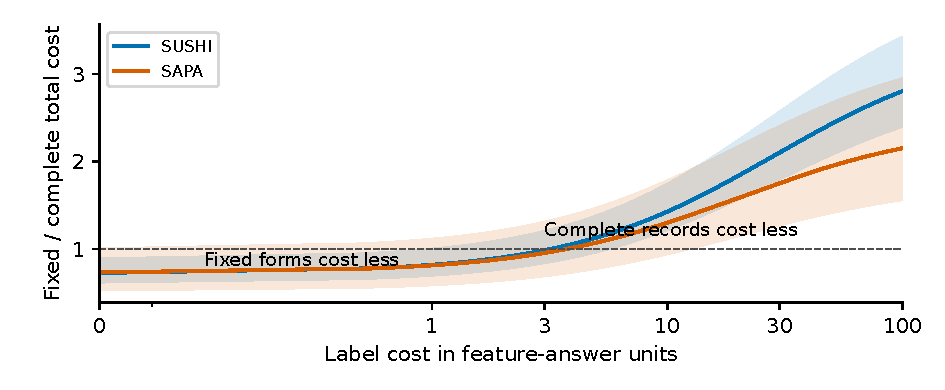
\includegraphics[width=.85\textwidth]{figures/cost_choice.pdf}
\caption{Fixed-form versus complete-record cost on all 70 controlled tree
tasks, allowing complete acquisition. Lines are medians, bands are the
10th--90th percentiles. Planning targets half-width 0.025, includes integer
sample counts and a minimum of thirty, and conditions on the reference.
Under an immutable cap, the complete-record alternative is unavailable.
When branching can compute the target and is permitted, its lower feature
count and full-information variance make it the natural comparator.}
\label{fig:costchoice}
\end{figure}
At zero label cost the median planned fixed/complete ratios are 0.726 on
SUSHI and 0.731 on SAPA; at label cost ten they are 1.427 and 1.299.
These conditional cost curves do not price an independent complete
reference as free: same-population reference records should first be used
as audit observations. Transferred or restricted calibration requires its
own analysis. An uncorrected imputation method cannot be assigned a
universal winning region using label cost alone, because its bias,
sample size and desired inference guarantee also matter.

\section{When Asking Changes the Answer}\label{app:measurement}
Let $P$ describe latent complete records and let $K_T$ be the distribution
of the recorded transcript given a latent record under form $T$. A frozen
score estimates
\[
 \widetilde\Delta_{q,K}
   =\E_{P,q,K_T}H_T(O_T),
\]
which can differ from the latent $\Delta=\E_P[Yd(X)]$. A branching policy
has its own sequential measurement kernel and hence its own mean score.
Pointwise unbiasedness for unchanged answers does not equate these means
under arbitrary collection-specific kernels. Randomized common anchors
identify mode or position differences for those anchors; identifying the
latent target additionally needs a measurement model or a reference.

We perform an exact semi-synthetic sensitivity calculation on the ten
binary tasks. At query position $j=1,\ldots,6$, independently flip the
answer with probability $\epsilon(j-1)/5$, for
$\epsilon\in\{0,0.01,0.03,0.05,0.1\}$. Labels are unchanged. Fixed forms
ask coordinates in increasing index order. Branching routes on the
\emph{recorded} noisy answers and stops at its leaf; its probability output
and old stump both use those answers. We sum all $2^6$ flip patterns to
obtain exact conditional first and second score moments, averaging over
people and fixed-form assignment. This is an illustrative position model,
not an estimated response-error process for either source survey.

\begin{table*}[t]
\centering
\caption{Position-dependent flips, integrated exactly over every noise pattern. Median absolute latent-target bias and bias divided by the clean branching standard error at $n=1000$. The final-position error rate is $\epsilon$; earlier rates increase linearly from zero.}
\label{tab:measurement}
\small
\setlength{\tabcolsep}{4pt}
\begin{tabular}{lrrrr}
\toprule
Data & $\epsilon$ & Method & Median $|\mathrm{bias}|$ & Bias / clean SE \\
\midrule
SUSHI & 0.00 & Branching & 0.00000 & 0.000 \\
SUSHI & 0.00 & Form scores & 0.00000 & 0.000 \\
SUSHI & 0.03 & Branching & 0.00076 & 0.164 \\
SUSHI & 0.03 & Form scores & 0.00095 & 0.203 \\
SUSHI & 0.10 & Branching & 0.00247 & 0.527 \\
SUSHI & 0.10 & Form scores & 0.00309 & 0.663 \\
SAPA & 0.00 & Branching & 0.00000 & 0.000 \\
SAPA & 0.00 & Form scores & 0.00000 & 0.000 \\
SAPA & 0.03 & Branching & 0.00233 & 0.537 \\
SAPA & 0.03 & Form scores & 0.00187 & 0.455 \\
SAPA & 0.10 & Branching & 0.00777 & 1.787 \\
SAPA & 0.10 & Form scores & 0.00621 & 1.513 \\
\bottomrule
\end{tabular}
\end{table*}


At a last-position flip probability of 0.1, median absolute bias in units
of a clean branching standard error at $n=1000$ is 0.53/0.66 for
branching/form scores on SUSHI and 1.79/1.51 on SAPA. Thus a measurement
effect can dominate the sampling gain, and neither design is uniformly
more robust in this model. Repeating a fixed biased score at larger $n$
reduces its sampling variance but leaves its measurement bias unchanged.


\section{A Feasibility-First Workflow for Nonlinear Updates}\label{app:workflow}
Fix a profile space, an acquisition menu, a confidence level $1-\alpha>1/2$,
and a target half-width $e$. The workflow separates two certificates:
a dual lower bound $\delta_L$ on the identification floor and a feasible
approximation $v\in\Hh_\A$ with residual at most $\varepsilon$.
Only the second certificate permits an accuracy guarantee.

\paragraph{Rejecting an insufficient cap.}
If $\delta_L>e$, no interval with half-width at most $e$ can have uniform
coverage $1-\alpha$, for any number of records. To see this on a finite
space, choose a dual signed measure $h$ with $\|h\|_1=1$,
$h\perp\Hh_\A$, and $\sum_xh(x)d(x)>e$.
Define
\[
 P_\pm(x,y)=\frac{|h(x)|\pm yh(x)}2.
\]
Every interview cell has the same joint probability with $Y$ under the
two laws because its sum of $h$ is zero. This also gives identical
experiments under sequential design. Their target values are opposite
and more than $2e$ apart. Under the common observation law an interval
of that width cannot cover both, so the two coverage probabilities sum
to at most one. This rules out uniform coverage greater than one half.
The conclusion assumes arbitrary joint laws on the stated profile space;
a substantively justified restriction on those laws changes the problem.

\paragraph{Passing with a certified approximation.}
Suppose an observable score $H$ has conditional mean $Yv(X)$ and satisfies
$|H|\le C$. Conditional on all model fitting and calibration, fresh iid
records satisfy
\[
 \Pr_P\!\left\{|\overline H-\Delta(P)|
 \le\varepsilon+C\sqrt{2\log(2/\alpha)/n}\right\}\ge1-\alpha.
\]
This is Hoeffding's inequality plus
$|\E_P[Y(v-d)]|\le\varepsilon$. It is valid for every population on the
certified space, not merely the reference population used to fit a score.
For $\varepsilon<e$, the sufficient count in Section~2 follows by inversion.
If the lower and upper certificates straddle $e$, they have not resolved
feasibility: improve the approximation or compare a larger cap.

On a binary cube, write $v=\sum_{|S|\le b}\gamma_S\chi_S$ and
$C=\sum_S|\gamma_S|$. Query term $S$ with probability $|\gamma_S|/C$ and
return $CY\operatorname{sgn}(\gamma_S)\chi_S(X)$. The empty term uses no
feature; if $C=0$, return zero. This yields the required observable score and bound. The
finite-sample radius can therefore be minimized by a linear program:
\[
 \min_{\gamma,\varepsilon\ge0}
 \varepsilon+\sqrt{2\log(2/\alpha)/n}\|\gamma\|_1,
 \qquad |d-\mathsf F\gamma|\le\varepsilon\mathbf1,
\]
where only $\varepsilon$ is constrained nonnegative and $\gamma$ is free.
This is a conservative confidence criterion, distinct from the MSE
criterion in Appendix~\ref{app:dense}.

\paragraph{What scales without full form enumeration.}
The all-form search certifies an offline benchmark; deployment of an
already fitted score requires no such search. If a frozen contrast has
a supplied decomposition $d=\sum_j w_j f_j$, with each $f_j$ computable
within $b$ queries and $|f_j|\le M_j$, choose $j$ with probability
$|w_j|M_j/C$ for $C=\sum_j|w_j|M_j$ and return
$CY\operatorname{sgn}(w_j)f_j/M_j$.
It is exactly unbiased and bounded by $C$. This includes differences of
probability-averaging forests with depth at most $b$, even when their
combined prediction uses many coordinates and the inputs are continuous.
A fixed form can simulate a sampled component by its path-set construction.
Neither method asserts optimal efficiency. Nonlinear transformations of
ensemble scores, including the logistic link in ordinary GBDT probability
outputs, need a separate approximation certificate.

For an arbitrary continuous model, restrict selected coordinates to two
values and hold the others fixed. The restriction of any $b$-coordinate
observable function has Boolean degree at most $b$. Thus a bias-floor
lower certificate on that finite slice is also a lower bound on the full
product-domain problem. The slice supplies no full-domain upper bound.
This is a one-sided rejection tool whose scope must be stated explicitly.

\subsection{Independent GBDT and Neural-Network Versions}\label{app:nonlinear}
WDBC contains 569 diagnostic records and 30 image-derived continuous
features \citep{wolberg1993}. The target is malignant versus benign.
The data therefore supply a non-questionnaire outcome and continuous
model inputs, but their image-derived acquisition does not instantiate
our survey cap. This experiment asks about mathematical feasibility for
ordinary model classes.

Five fixed seeds, 20261108--20261112, permute the data. The first 100
records train the old model; the next 300 train the new model; the last
169 determine its evaluated accuracy gain. GBDT uses 30 versus 100 trees,
depth two, learning rate 0.05 and minimum leaf size five. The MLP uses
one ReLU hidden layer of width eight versus sixteen, $\ell_2$ penalty one,
and L-BFGS. Each model's standardization uses its own training records.
No evaluation record selects model size, variables, thresholds or seed. The splits reuse individuals and are descriptive sensitivity analyses, not independent populations.

The discrete condition takes twelve coordinates at equally spaced indices
of the original feature list and thresholds them at medians of the 400
training records. Both probability outputs and deterministic thresholds
at one half are evaluated. The admissible domain is the entire binary
cube, with $b=3$. The continuous condition trains on all thirty original
features. Its certificate varies the same twelve coordinates between
their training first and third quartiles and fixes the others to training
medians. Continuous-condition brackets refer to that slice; only their
lower endpoints apply to the full domain. Arbitrary product combinations
can violate empirical feature dependencies, so these are distribution-free
certificates under the declared domain, not support-aware clinical claims.

For a target vector $d$ on the 4,096-profile grid and the degree-three
Walsh matrix $\mathsf F$, the floor program minimizes
$\|d-\mathsf F\gamma\|_\infty$. Its floating-point solution is converted
to certificates: round primal coefficients to multiples of $2^{-28}$;
round a dual vector to integers $z$ on scale $2^{40}$; then form
\[
 h_{\rm int}=4096z-\mathsf F\mathsf F^Tz.
\]
Because $\mathsf F^T\mathsf F=4096I$, the integer vector has exactly zero
degree-at-most-three coefficients. Dividing by its exact $\ell_1$ norm
gives a feasible rational dual. Both its inner product with the stored
binary64 predictions and the rounded primal's maximum residual are
computed with rational arithmetic. The certificate treats those stored
software predictions as the defined finite target, without claiming
formal verification of a real-arithmetic neural network.

The binary probability condition also minimizes the bias-expanded
Hoeffding radius at $n=1000$, $\alpha=.05$. The exact certificates do not
depend on an optimizer's success flag. A bounded-time implementation can
fall back to a feasible low-degree projection and its orthogonal residual;
solver status and certificate width are released in every row.
All thirty floor programs terminated optimally in the released run. The
largest certified bracket width is below $10^{-7}$, and the fitted models
emitted no convergence warnings.

\begin{table*}[t]
\centering
\caption{Cap-three nonlinear-model diagnostic. Binary rows bracket the full binary-domain floor. Continuous rows bracket a twelve-coordinate slice; only the lower endpoints transfer to the full continuous domain. The last column compares the certified floor directly with the requested half-width.}
\label{tab:nonlineardetail}
\small
\setlength{\tabcolsep}{4pt}
\begin{tabular}{lrrrr}
\toprule
Model condition & Splits & Median LB & Median UB & LB$>0.025$ \\
\midrule
Binary, probability, GBDT & 5 & 0.0552 & 0.0552 & 5/5 \\
Binary, probability, MLP & 5 & 0.2780 & 0.2780 & 5/5 \\
Binary, threshold, GBDT & 5 & 0.3409 & 0.3409 & 5/5 \\
Binary, threshold, MLP & 5 & 0.6572 & 0.6572 & 5/5 \\
Continuous slice, GBDT & 5 & 0.0065 & 0.0065 & 0/5 \\
Continuous slice, MLP & 5 & 0.1286 & 0.1286 & 5/5 \\
\bottomrule
\end{tabular}
\end{table*}


The continuous slice results are weaker statements than the complete
binary-cube results. A small slice lower bound cannot certify an acceptable
full-domain bias. Similarly, reporting a good empirical MSE does not
replace the uniform residual required for a bias-expanded interval.

\section{Proper Scores and Pairwise Targets}\label{app:metrics}
The score-design method applies to a bounded known record-level target
$t(x,y)$, without requiring that it be a randomized classification gain.
For a label observed separately, write
\[
 t(x,y)=a(x)+yc(x),\qquad
 a(x)=\frac{t(x,1)+t(x,-1)}2,\quad
 c(x)=\frac{t(x,1)-t(x,-1)}2.
\]
On a finite domain, identification under arbitrary joint populations is
equivalent to $a,c\in\Hh_\A$. On the full binary cube with cap $b$, this is
$\deg(a),\deg(c)\le b$. Indeed the observation span on $(x,y)$ is
$\Hh_\A\otimes\operatorname{span}\{1,y\}$: a table may have separate
entries for the two labels. Its orthogonal complement gives indistinguishable
populations whenever the target lies outside that span. In particular the
common identification criterion for fixed forms and branching still applies.

For $z=(y+1)/2$ and $d=p_1-p_0$, the improvement in Brier loss is
\[
 t_{\rm Br}(x,y)=(p_0-z)^2-(p_1-z)^2
                =d(1-p_0-p_1)+yd.
\]
Thus degree at most $r$ for each probability function implies degree at most
$2r$ for this target's feature-only component and at most $r$ for its label
component. The bound can be strict because terms cancel. The actual degree,
or a certified approximation residual, determines the necessary cap.
Doubling is attainable: take $p_0=1/2$ and
$p_1=1/2+\gamma(x_1x_2+x_3x_4)$, with $0<\gamma\le1/4$.
The accuracy contrast has degree two, whereas the Brier feature-only
component is $-2\gamma^2(1+x_1x_2x_3x_4)$ and has degree four.
For a common depth-$b$ tree whose leaf values determine both probabilities,
the complete loss difference is still computable along that same path.

For log loss, clip each probability to a fixed interval
$[\eta,1-\eta]$, $0<\eta<1/2$, before defining the target. Then
\[
 \begin{split}
 a_{\log}&=\tfrac12\log\frac{p_1(1-p_1)}{p_0(1-p_0)},\\
 c_{\log}&=\tfrac12\log\frac{p_1(1-p_0)}{p_0(1-p_1)}.
 \end{split}
\]
These formulas estimate improvement of the clipped rules. A logarithm of
an ensemble average can introduce interactions of every order, even when
each probability has a low-degree representation. A common tree partition
again avoids that issue because the transformed values are constant on leaves.

The full-form program in Section~\ref{sec:pathdesign} replaces its
right-hand side by $\widehat t_y(S)$ for each label. Its pointwise identity,
population-specific variance objective, and invariance of unbiasedness to
calibration error remain unchanged. The symmetric-label minimax formula
$V(d,\A)$ and its sharp ratio were proved for $Yd(X)$; this extension of
the estimator does not assert that the identical formula is the global
minimax coefficient for every proper score. The path simulation does preserve
any bounded target's conditional mean and multiplies its conditional
second moment by at most the number of padded path sets.

\paragraph{AUC needs a pair design.}
Let $X^+\sim P(X\mid Y=1)$ and $X^-\sim P(X\mid Y=-1)$ be independent.
For a frozen score $s$, define
$k_s(x^+,x^-)=\mathbf1\{s(x^+)>s(x^-)\}
+\tfrac12\mathbf1\{s(x^+)=s(x^-)\}$.
The AUC difference is $\E[k_{s_1}-k_{s_0}]$ under the product of these two
conditional laws. Disjoint labeled case--control pairs give iid pair targets;
one can design unbiased scores on pair transcripts, retaining a separate
cap on each member. This differs from a single-record target: using all
case--control pairs introduces U-statistic dependence, and the sharp
single-record coefficient ratio cannot be asserted for that design.
Class prevalence, label-screening cost and the availability of both classes
must also enter an acquisition comparison. We establish the record-level
Brier/log-loss extension here and leave pair-design optimality unclaimed.

\section{Binary Experiments and the Budget Curve}\label{app:sign}
\paragraph{The binomial minimax value.}
For any nonzero $d$ set $M=\|d\|_\infty$. With full profiles a randomized sign with conditional mean $Yd(X)/M$ has population mean $\Delta/M$. For $n$ iid signs $W_i$ with unknown mean $\mu_0$, the estimate $\sqrt n\,\overline W/(1+\sqrt n)$ has variance $(1-\mu_0^2)/(1+\sqrt n)^2$ and squared bias $\mu_0^2/(1+\sqrt n)^2$. For the lower bound fix a profile at which $|d|=M$ and vary the sign label. A $\mathrm{Beta}(\sqrt n/2,\sqrt n/2)$ prior on the success probability of the sign makes this constant-risk rule its posterior mean on the mean-sign scale. The Bayes risk equals the displayed frequentist risk, proving minimaxity. The full-profile value is therefore $M^2/(1+\sqrt n)^2$. The one-feature construction in Proposition~\ref{prop:add} simulates these same signs, and the constant-profile lower bound applies. For $M=0$ return zero.

\subsection{Proof of Theorem~\ref{thm:gap}}\label{app:gap}
If $b<2k$, under uniform $X$ the laws $Y=\pm d_k(X)$ give the same observations on every allowed leaf. The risk is at least one and zero attains it. For $b\ge2k$ we show that $J_\U(d_k)=1/C$ and construct a per-person score $H$ with $\E[H\mid X,Y]=Yd_k(X)$ and $\E[H^2\mid X,Y]=C$ for each design type.

\paragraph{Fixed forms.}
Under the uniform law, projecting a multilinear expansion onto a mask retains exactly its contained Fourier terms. In a block of size four a mask with $j=2,3,4$ coordinates captures at most $1/4,1/2,1$ of the total squared coefficient mass, respectively. The first maximum is achieved by a supported pair and the other two by any mask of the indicated size. A block with fewer than two coordinates captures zero mass. Independence of blocks gives total mass at most $2^{b-4k}$, and choosing a supported pair in every two-coordinate block attains it for any budget allocation assigning between two and four coordinates to every block. For two coordinates sample one of four supported pairs uniformly and return twice its signed product. For three, choose $\{1,2,3\}$ or $\{2,3,4\}$ with equal probability. Return $2f$ when the first form is chosen and $x_2=x_3$, or when the second is chosen and $x_2\ne x_3$; return zero otherwise. For four the score is $f$ itself. The scores have conditional means $f$ and constant second moments $4,2,1$. Multiply independently randomized block scores and $Y$ to obtain the desired $H$.

\paragraph{Branching forms.}
When $b=2k+r$, $0\le r\le k$, evaluate $r$ blocks via branching, using three queries each; use a random signed pair score of magnitude two in every other block. Then $H$ has constant absolute value $2^{k-r}$ and square $C=4^{k-r}$. When $b\ge3k$, evaluate every block. For the lower witness, at any deterministic leaf under uniform $X$, an unqueried coordinate remains uniform independent of the others. Nonzero conditional mean for the product requires that every block has at least two exposed coordinates. At most $r$ blocks have more than two, so $|\E_\U[d_k\mid\ell]|\le2^{-(k-r)}$. Averaging yields the bound on $J$. It is attained by evaluating $r$ blocks exactly and querying one predetermined supported pair in each other block. The absolute conditional mean is then $2^{-(k-r)}$ at every leaf.

\paragraph{Exact program and leading coefficients.}
The witness $\mu=\U,h=d_k$ in \eqref{eq:dual} gives $\Phi_n\ge1/(1+n/C)$. Randomized query procedures can be represented as mixtures over deterministic interviews by drawing all their random coins in advance. Taking their unbiased transcript scores with shrinkage $\gamma=n/(n+C)$ gives $s_g=\gamma d_k$ and a second-moment contribution at most $\gamma^2 C$ at every profile. Thus $\Phi_n\le(1-\gamma)^2+\gamma^2 C/n=C/(n+C)$. The same witness in \eqref{eq:vdual} and the unshrunk scores give $V=C$. Theorem~\ref{thm:finite} yields the nonasymptotic rates. At $b\ge3k$, evaluating $d_k$ yields a sign of mean $\Delta$ and the binomial minimax value above.

\paragraph{Exact binary comparison for branching.}
For $2k\le b\le3k$ put $\lambda=2^{b-3k}$. The branching score $\lambda H$ is a sign with mean $\lambda\Delta$ for every $P$. Conversely consider the subfamily of uniform $X$ with conditional label law $(1+\theta y d_k(x))/2$. Then $\Delta=\theta\in[-1,1]$. At each leaf, conditionally on the history and independent random coins, $p_\theta(z)=p_0(z)(1+\theta s_z)$ with $|s_z|\le\lambda$ and $\sum_zp_0(z)s_z=0$. A sign $w$ of mean $\lambda\theta$ can generate this leaf via the probability kernel $K(z\mid w)=p_0(z)(1+w s_z/\lambda)$. Simulating the leaves successively reproduces the complete protocol. This is an explicit experiment comparison in the sense of \citet{blackwell1953}: on the indicated subfamily an arbitrary interview can be simulated using the scalar sign. Together with the construction for every $P$, it gives exact equality of minimax risks with the binary-mean experiment, even for biased estimators.

\paragraph{Why the population supremum matters.}
A uniform-law calculation can be uninformative even when an update is identifiable. For example, take an extra switch $z\in\{-1,1\}$ and set $\widetilde d=1+\mathbf1\{z=1\}(d_k-1)$. This remains Boolean, has degree $2k+1$, and has uniform mean $1/2$, so even an empty form captures at least $1/4$ of the squared mean signal in the uniform witness $h=\widetilde d$. At the identifiable width $2k+1$, however, a population supported on $z=1$ contains the original hard experiment at that width. An auditor given the switch for free still has branching risk of order $\min\{1,4^{k-1}/n\}$ for $k\ge1$. Optimizing over profile laws and perturbations in \eqref{eq:dual} accounts for this possibility.

\begin{figure}[t]
\centering
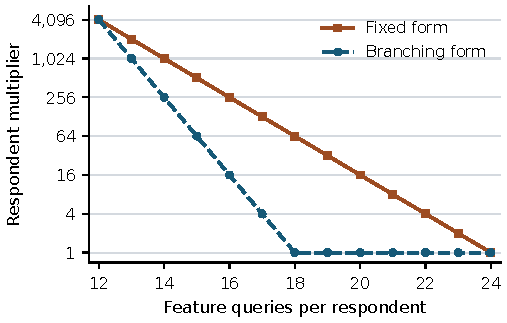
\includegraphics[width=.62\textwidth]{figures/query_cost.pdf}
\caption{Exact synthetic budget curve for the same update on 24 features ($k=6$). The fixed coefficient is 64 and the branching coefficient is one at 18 queries.}
\label{fig:cost}
\end{figure}


\section{Reproducibility and Research Methods}\label{app:repro}
The anonymous supplement contains code, numerical certificates, aggregate
results, simulation standard errors, and figure/table generators. Source data
are obtained separately with pinned checksums. The SUSHI loader also verifies
a normalized profile fingerprint because the creator's legacy archive and
current PrefLib profile differ. Individual SUSHI rankings may not be
redistributed; no individual survey records are supplied.

Checks cover 21,276 exact rational hybrid-budget inequalities, six independent
small conic programs, binary and ordinal profile-cell formulations, and five
full-support local-efficiency comparisons. EM is checked against direct
maximization of its penalized likelihood. Release checks verify task counts,
comparator populations, primal/dual bounds, pilot-risk accounting, and
interval simulation errors. Symbolic and numerical checks are also supplied.

These finite checks support the implementations and written derivations;
they do not replace proofs of general statements. The product counterexample
has a separately released rational certificate checked exactly on all 256
profiles. The unrestricted-menu experiment enumerates every eligible form
on all 70 binary tasks and releases its population witnesses. Nonlinear-model
floor certificates use exact integer nullspace checks and rational endpoint
evaluation on the released prediction grids. The one-sided address formula
has an analytic proof and exact small-instance primal/dual checks.
All 1,048 retained release checks and 50 new archive/forest checks pass.
The new checks verify actual-form observability, the Brier block
decomposition, MI summary arithmetic and the complete forest grid,
including a separate address instance with known optima. The proper-loss extension is
checked on every profile and both labels of
an independent toy cube. The budget-curve release contains all 260
recorded cap/contrast cases, with separately implemented Python-integer
Walsh and rational endpoint checks; age-transfer summaries retain every
nonzero case and explicitly record zero contrasts.


\paragraph{Additions in this version.}
The code for the exact cap grid, the smoothing and resampling sensitivity, the model-assisted imputation comparison and the reference-law predictor is released with per-task JSON results and logs. Public mirrors were used for the UCI files (PMLB for Spambase and Ionosphere, GitHub mirrors for the thyroid files, a Git LFS mirror of the Kaggle release of the CDC diabetes indicators); each mirror was verified by reproducing released numbers exactly. Monte Carlo checks of the potential inequality~\eqref{eq:potential} and of greedy $r$-round strategies on pointer trees of depth $3$ to $10$ accompany the proof of Theorem~\ref{thm:binarytree}. Material from earlier stages of the study is collected in a separate supplementary report with its own tables. A generative language model participated in formulating research questions, deriving and checking proof arguments, implementing analyses, and drafting the manuscript; the authors remain responsible for all content.


\end{document}
